\documentclass[a4paper, 11pt, twoside=semi]{scrartcl}

\usepackage[utf8]{inputenc}
\usepackage[english]{babel}

\usepackage{enumerate}

% Deutsche Silbentrennung
%\usepackage[ngerman]{babel}

% Typische Mathesymbole etc, was man oft braucht
\usepackage{textcomp}
\usepackage{latexsym}
\usepackage{amssymb}
\usepackage{amsmath}
\usepackage{wasysym}
%\usepackage{txfonts}

% Teilfiguren in figure Umgebungen erlauben%
\usepackage{subfig}
\usepackage{float}
\restylefloat{figure}

% Schrift die mit Zeichencodierung klar kommt
%\usepackage{lmodern}




% Bilder einfügen
\usepackage{graphicx}
% Quelltext einfügen
\usepackage{verbatim}
%allows multiple rows and colums in a tabular environment
\usepackage{array}
%\usepackage{multirow}
\usepackage{multicol}


%fancy haedings
%\usepackage{fancyhdr}
%\pagestyle{fancy}

% Definitionen von Farben
\usepackage{xcolor}
\definecolor{LinkColor}{rgb}{0,0,0.5}
\definecolor{blue}{rgb}{0,0,1}
% \definecolor{dkgreen}{rgb}{0,0.6,0}
% \definecolor{gray}{rgb}{0.5,0.5,0.5}
% \definecolor{mauve}{rgb}{0.58,0,0.82}

% Einf\"ugen von Tikz grafiken
\usepackage{booktabs}
\usepackage{pgf}
\usepackage{tikz}
\usetikzlibrary{shapes,backgrounds,mindmap,trees,calc}

\usepackage{pgfplots}
\usepackage{pgfplotstable}
\usepgfplotslibrary{colormaps}
\usepgfplotslibrary{colorbrewer}
\pgfplotsset{compat=1.15} %
\pgfplotsset{cycle list/Spectral}

%\usepackage{filecontents}

\newcounter{piea}
\newcounter{pieb}
\newcounter{piec}
\newcounter{pied}
\newcounter{piee}
\newcounter{pief}
\newcounter{pieg}
\newcounter{pieh}



% Definitionen f\"ur Spiderweb chart
\newcommand{\D}{5} % number of dimensions (config option)
\newcommand{\U}{100} % number of scale units (config option)
\newcommand{\US}{5}   % number of scale units shown (config option)
\newdimen\R % maximal diagram radius (config option)
\R=2cm 
\newdimen\L % radius to put dimension labels (config option)
\L=3cm
\newcommand{\A}{360/\D} % calculated angle between dimension axes  
\newcommand{\SU}{\U/\US} % calculated distance between shown axes  
\newcommand{\createradar}{
  \path (0:0cm) coordinate (O); % define coordinate for origin
  % draw the spiderweb
  \foreach \X in {1,...,\D}{ \draw [opacity=.5] (\X*\A+90:0) -- (\X*\A+90:\R); }%
  \foreach \Y in {0,...,\U}{ \foreach \X in {1,...,\D}{ \path (\X*\A+90:\Y*\R/\U) coordinate (D\X-\Y); } } %
  \foreach \Y in {0,...,\US}{ \foreach \X in {1,...,\D}{ \path (\X*\A+90:\Y*\SU*\R/\U) coordinate (A\X-\Y); \fill [opacity=0.5] (A\X-\Y) circle (1pt); }%
                              \draw [opacity=0.5] (0+90:\Y*\SU*\R/\U) \foreach \X in {1,...,\D}{ -- (\X*\A+90:\Y*\SU*\R/\U)  } -- cycle; }%  
  %create correct width
  \draw [color=white] (-5,2) -- (5,2);%
  % define labels for each dimension axis (names config option)
  \path (1*\A+90:\L) node (L1) {\small Heterogenit\"at};%
  \path (2*\A+90:.85\L) node (L2) {\small Verteilung};%
  \path (3*\A+90:.87\L) node (L3) {\small Zeitabh\"angigkeit};%
  \path (4*\A+90:\L) node (L4) {\small Dynamik};%
  \path (5*\A+90:.8\L) node (L5) {\small Komplexit\"at};%  
}

% Definition for Pie-Chart
\newcommand{\slice}[5]{%
  \pgfmathparse{0.5*#1+0.5*#2}%
  \let\midangle\pgfmathresult%
  % slice
  \draw[thin,fill=#5,draw=white] (0,0) -- (#1:1) arc (#1:#2:1) -- cycle;%
  % outer label
  \node[label=\midangle:#4] at (\midangle:1) {};%
  % inner label
  \pgfmathparse{min((#2-#1-10)/110*(-0.3),0)}%
  \let\temp\pgfmathresult%
  \pgfmathparse{max(\temp,-0.5) + 0.8}%
  \let\innerpos\pgfmathresult%
  \node at (\midangle:\innerpos) {#3};%
}

%Definition of Box-Plots
\newcommand{\boxplot}[6]{%
	%#1: center, #2: median, #3: 1/4 quartile, #4: 3/4 quartile, #5: min, #6: max
	\filldraw[fill=blue!30,draw=blue,line width=.2mm] let \n{boxxl}={#1-0.3}, \n{boxxr}={#1+0.3} in (axis cs:\n{boxxl},#3) rectangle (axis cs:\n{boxxr},#4);   % draw the box
	\draw[line width=1mm, color=blue] let \n{boxxl}={#1-0.3}, \n{boxxr}={#1+0.3} in (axis cs:\n{boxxl},#2) -- (axis cs:\n{boxxr},#2);             % median
	\draw[line width=.2mm] (axis cs:#1,#4) -- (axis cs:#1,#6);                                                                           % bar up
	\draw[line width=.2mm] let \n{whiskerl}={#1-0.15}, \n{whiskerr}={#1+0.15} in (axis cs:\n{whiskerl},#6) -- (axis cs:\n{whiskerr},#6);        % upper quartile
	\draw[line width=.2mm] (axis cs:#1,#3) -- (axis cs:#1,#5);                                                                           % bar down
	\draw[line width=.2mm] let \n{whiskerl}={#1-0.15}, \n{whiskerr}={#1+0.15} in (axis cs:\n{whiskerl},#5) -- (axis cs:\n{whiskerr},#5);        % lower quartile
}


% Definition der Befehle todo und todoln fuer Hinweistexte
%\newcommand\todo[1]{\fbox{\scriptsize\textbf{#1}}}
%\newcommand\todoln[1]{\fbox{\parbox{.9\linewidth}{\scriptsize\textbf{#1}}}}


\author{Thomas Kühn}
\title{Evaluation @ ECSA}


\begin{document}



\section{Research Objects}

%\subsection{Histogramm f\"ur Research Object (75)}
%\begin{figure}
\begin{center}
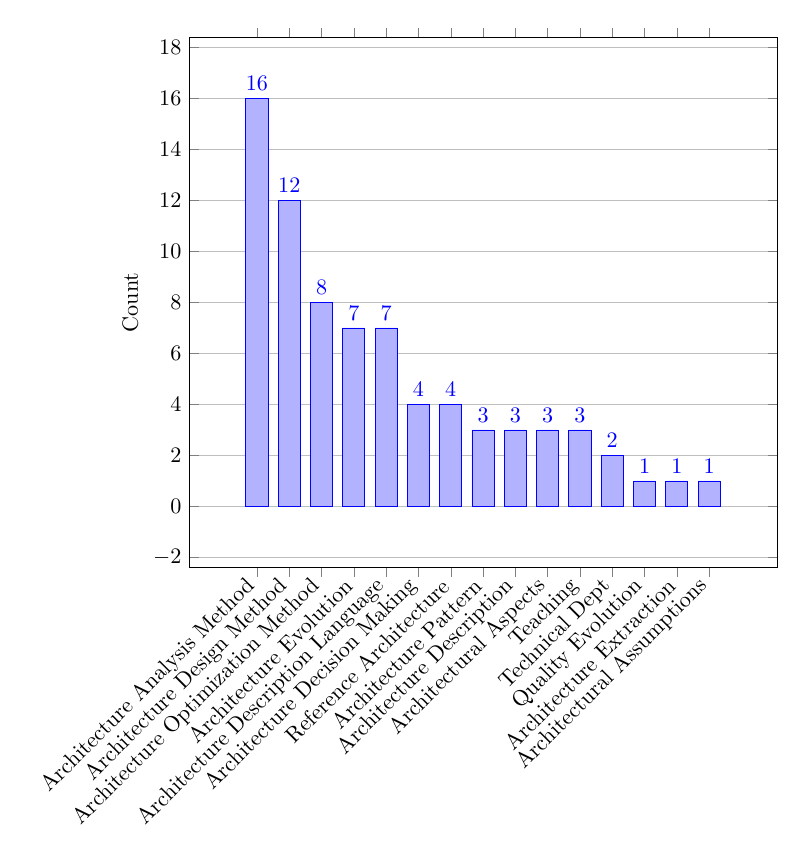
\begin{tikzpicture}[scale=.8]
\begin{axis}[ ybar, ymajorgrids, enlargelimits=0.15, legend style={at={(0.5,-0.15)}, anchor=north,legend columns=-1},
    width=.90\linewidth,height=10cm,
    nodes near coords, %nodes near coords align=below,
    ylabel={Count}, ymin=0,
    x tick label style={rotate=45,anchor=east},
    xtick={1,2,3,4,5,6,7,8,9,10,11,12,13,14,15},
    xticklabels={Architecture Analysis Method,Architecture Design Method,Architecture Optimization Method,Architecture Evolution,Architecture Description Language,Architecture Decision Making,Reference Architecture,Architecture Pattern,Architecture Description,Architectural Aspects,Teaching,Technical Dept,Quality Evolution,Architecture Extraction,Architectural Assumptions
}
    %xlabel={Research Object}    
    ]
  \addplot coordinates { (1,16)  (2,12)  (3,8)  (4,7)  (5,7)  (6,4)  (7,4)  (8,3)  (9,3)  (10,3)  (11,3)  (12,2)  (13,1)  (14,1)  (15,1)   };
\end{axis}
\end{tikzpicture}
\end{center}
%\caption{Histogramm f\"ur Research Object (75)}
%\label{fig:histo_researchobject}
%\end{figure}


%\subsection{Histogramm f\"ur Year (71)}
%\begin{figure}
\begin{center}
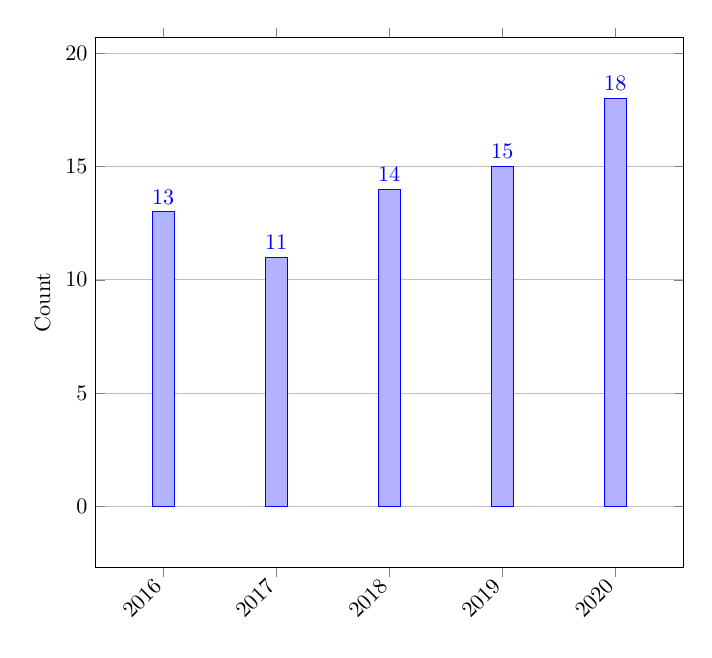
\begin{tikzpicture}[scale=.8]
\begin{axis}[ ybar, ymajorgrids, enlargelimits=0.15, legend style={at={(0.5,-0.15)}, anchor=north,legend columns=-1},
    width=.90\linewidth,height=10cm,
    nodes near coords, %nodes near coords align=below,
    ylabel={Count},ymin=0,
    x tick label style={rotate=45,anchor=east},
    xtick={1,2,3,4,5},
    xticklabels={2016,2017,2018,2019,2020
}
    %xlabel={Year}    
    ]
  \addplot coordinates { (1,13)  (2,11)  (3,14)  (4,15)  (5,18)   };
\end{axis}
\end{tikzpicture}
\end{center}
%\caption{Histogramm f\"ur Year (71)}
%\label{fig:histo_year}
%\end{figure}



%\subsection{Pie chart for Research Object (75)}
%\begin{figure}
\begin{center}
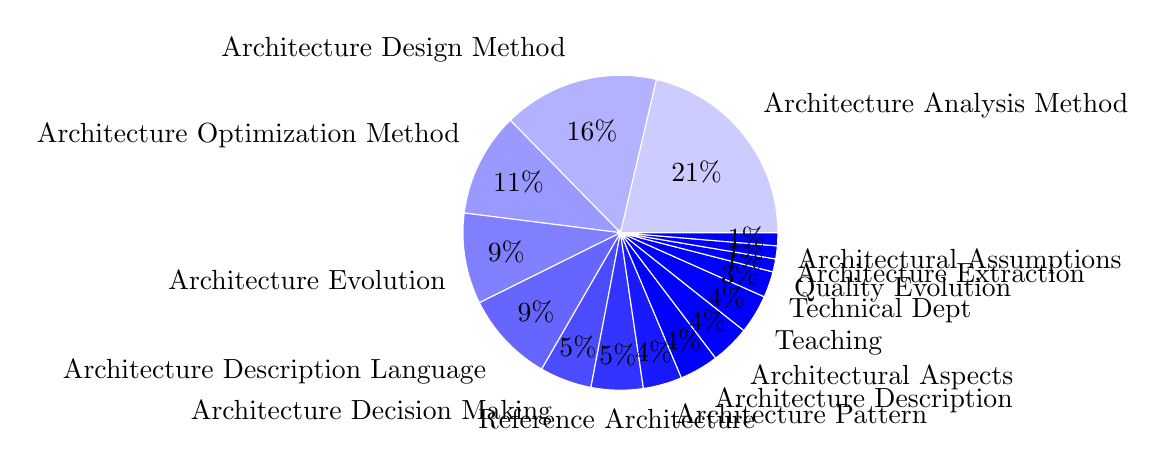
\begin{tikzpicture}[scale=2]
\pgfmathsetcounter{pieb}{0}
\foreach \p/\q/\t/\c in {21/16/Architecture Analysis Method/blue!20, 16/12/Architecture Design Method/blue!30, 11/8/Architecture Optimization Method/blue!40, 9/7/Architecture Evolution/blue!50, 9/7/Architecture Description Language/blue!60, 5/4/Architecture Decision Making/blue!70, 5/4/Reference Architecture/blue!80, 4/3/Architecture Pattern/blue!90, 4/3/Architecture Description/blue!100, 4/3/Architectural Aspects/blue!110, 4/3/Teaching/blue!120, 3/2/Technical Dept/blue!130, 1/1/Quality Evolution/blue!140, 1/1/Architecture Extraction/blue!150, 1/1/Architectural Assumptions/blue!160}
  {
    \setcounter{piea}{\value{pieb}}
    \addtocounter{pieb}{\q}
    \slice{\thepiea/75*360}
          {\thepieb/75*360}
          {\p\%}{\t}{\c}
  }
\end{tikzpicture}
\textbf{Pie chart for Research Object (75)}
\end{center}
%\caption{Pie chart for Research Object (75)}
%\label{fig:pie_researchobject}
%\end{figure}


\input{figs/chisto_year_researchobject}

\section{Evaluation Methods}

%\subsection{Histogramm f\"ur Evaluation Methods (87)}
%\begin{figure}
\begin{center}
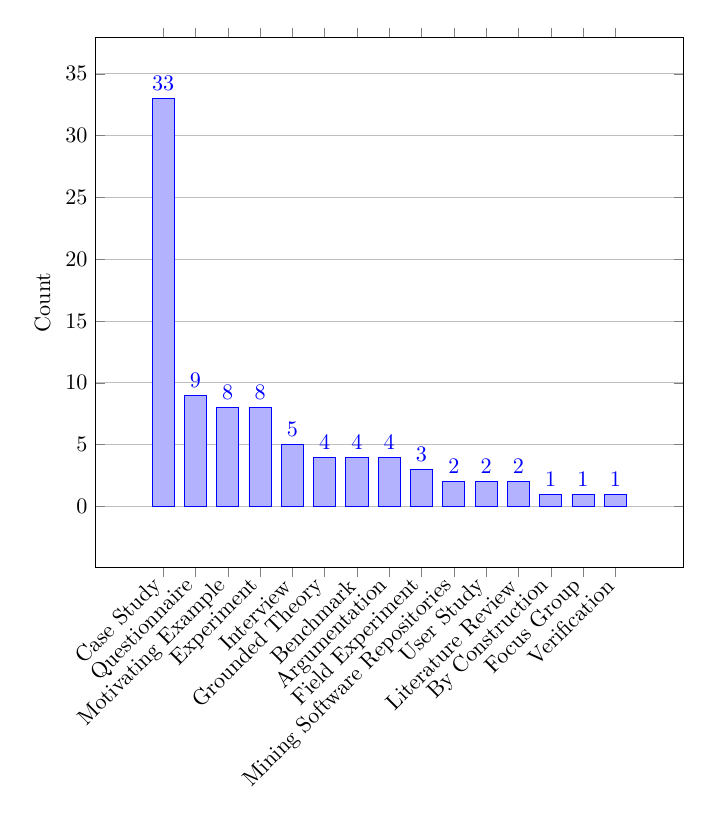
\begin{tikzpicture}[scale=.8]
\begin{axis}[ ybar, ymajorgrids, enlargelimits=0.15, legend style={at={(0.5,-0.15)}, anchor=north,legend columns=-1},
    width=.90\linewidth,height=10cm,
    nodes near coords, %nodes near coords align=below,
    ylabel={Count},ymin=0,
    x tick label style={rotate=45,anchor=east},
    xtick={1,2,3,4,5,6,7,8,9,10,11,12,13,14,15},
    xticklabels={Case Study,Questionnaire,Motivating Example,Experiment,Interview,Grounded Theory,Benchmark,Argumentation,Field Experiment,Mining Software Repositories,User Study,Literature Review,By Construction,Focus Group,Verification
}
    %xlabel={Evaluation Methods}    
    ]
  \addplot coordinates { (1,33)  (2,9)  (3,8)  (4,8)  (5,5)  (6,4)  (7,4)  (8,4)  (9,3)  (10,2)  (11,2)  (12,2)  (13,1)  (14,1)  (15,1)   };
\end{axis}
\end{tikzpicture}
\end{center}
%\caption{Histogramm f\"ur Evaluation Methods (87)}
%\label{fig:histo_evaluationmethods}
%\end{figure}


%\subsection{Histogramm f\"ur Year (71)}
%\begin{figure}
\begin{center}
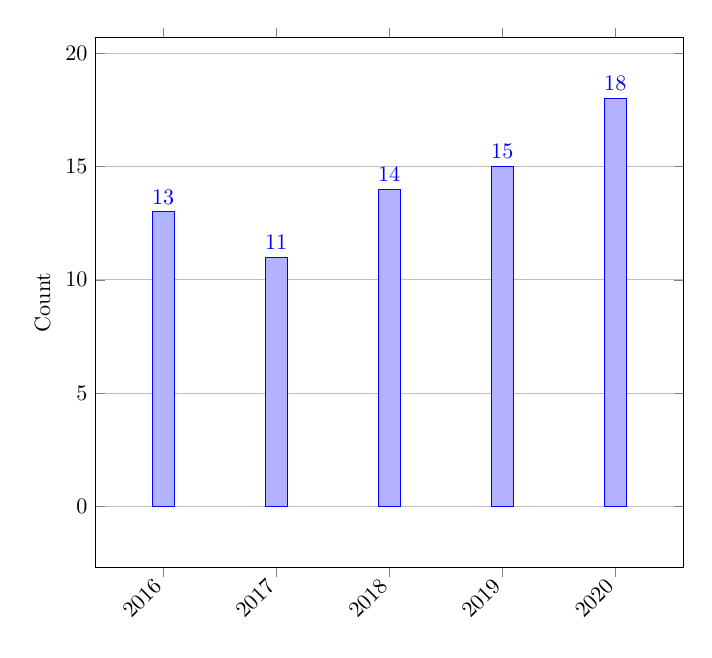
\begin{tikzpicture}[scale=.8]
\begin{axis}[ ybar, ymajorgrids, enlargelimits=0.15, legend style={at={(0.5,-0.15)}, anchor=north,legend columns=-1},
    width=.90\linewidth,height=10cm,
    nodes near coords, %nodes near coords align=below,
    ylabel={Count},ymin=0,
    x tick label style={rotate=45,anchor=east},
    xtick={1,2,3,4,5},
    xticklabels={2016,2017,2018,2019,2020
}
    %xlabel={Year}    
    ]
  \addplot coordinates { (1,13)  (2,11)  (3,14)  (4,15)  (5,18)   };
\end{axis}
\end{tikzpicture}
\end{center}
%\caption{Histogramm f\"ur Year (71)}
%\label{fig:histo_year}
%\end{figure}


\input{figs/chisto_year_evaluationmethods}
%\subsection{Portfolio f\"ur Research Object und Evaluation Methods (Gr\"o\ss{}e entspricht der Anzahl)}
%\begin{figure}
\begin{center}
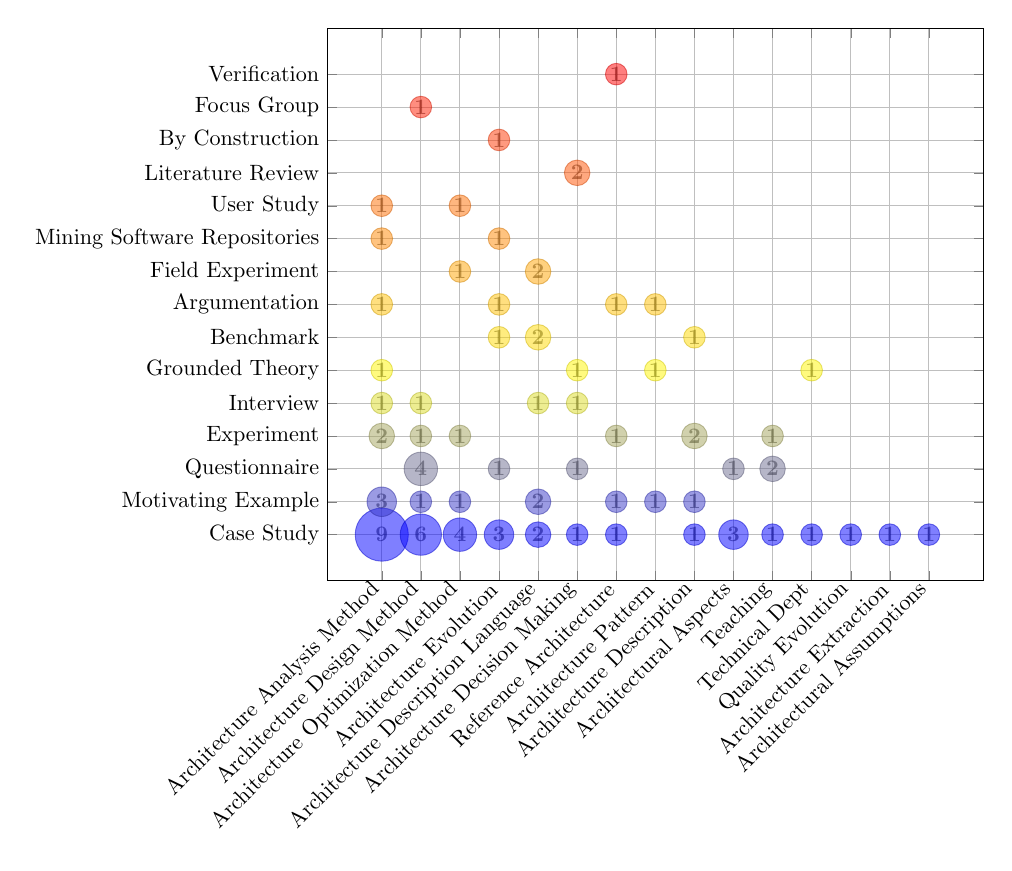
\begin{tikzpicture}[scale=.8]
\begin{axis}[scatter,
    width=.99\linewidth,
    cycle multi list=Spectral,
    every axis plot/.append style={draw, fill, fill opacity=0.5},
    scatter src=y,
    nodes near coords style={color=black,font=\small},
    %enlargelimits=0.15,
    x tick label style={rotate=45,anchor=east},
    xtick={0,1,2,3,4,5,6,7,8,9,10,11,12,13,14}, xticklabels={Architecture Analysis Method,Architecture Design Method,Architecture Optimization Method,Architecture Evolution,Architecture Description Language,Architecture Decision Making,Reference Architecture,Architecture Pattern,Architecture Description,Architectural Aspects,Teaching,Technical Dept,Quality Evolution,Architecture Extraction,Architectural Assumptions},
    ytick={0,1,2,3,4,5,6,7,8,9,10,11,12,13,14}, yticklabels={Case Study,Motivating Example,Questionnaire,Experiment,Interview,Grounded Theory,Benchmark,Argumentation,Field Experiment,Mining Software Repositories,User Study,Literature Review,By Construction,Focus Group,Verification},
    grid=both
]

\addplot[mark size=12.000,opacity=0.5,text=black] coordinates { (0,0) } node[text=black,font=\bfseries] {9};
\addplot[mark size=6.667,opacity=0.5,text=black] coordinates { (0,1) } node[text=black,font=\bfseries] {3};
\addplot[mark size=5.778,opacity=0.5,text=black] coordinates { (0,3) } node[text=black,font=\bfseries] {2};
\addplot[mark size=4.889,opacity=0.5,text=black] coordinates { (0,4) } node[text=black,font=\bfseries] {1};
\addplot[mark size=4.889,opacity=0.5,text=black] coordinates { (0,5) } node[text=black,font=\bfseries] {1};
\addplot[mark size=4.889,opacity=0.5,text=black] coordinates { (0,7) } node[text=black,font=\bfseries] {1};
\addplot[mark size=4.889,opacity=0.5,text=black] coordinates { (0,9) } node[text=black,font=\bfseries] {1};
\addplot[mark size=4.889,opacity=0.5,text=black] coordinates { (0,10) } node[text=black,font=\bfseries] {1};
\addplot[mark size=9.333,opacity=0.5,text=black] coordinates { (1,0) } node[text=black,font=\bfseries] {6};
\addplot[mark size=4.889,opacity=0.5,text=black] coordinates { (1,1) } node[text=black,font=\bfseries] {1};
\addplot[mark size=7.556,opacity=0.5,text=black] coordinates { (1,2) } node[text=black,font=\bfseries] {4};
\addplot[mark size=4.889,opacity=0.5,text=black] coordinates { (1,3) } node[text=black,font=\bfseries] {1};
\addplot[mark size=4.889,opacity=0.5,text=black] coordinates { (1,4) } node[text=black,font=\bfseries] {1};
\addplot[mark size=4.889,opacity=0.5,text=black] coordinates { (1,13) } node[text=black,font=\bfseries] {1};
\addplot[mark size=7.556,opacity=0.5,text=black] coordinates { (2,0) } node[text=black,font=\bfseries] {4};
\addplot[mark size=4.889,opacity=0.5,text=black] coordinates { (2,1) } node[text=black,font=\bfseries] {1};
\addplot[mark size=4.889,opacity=0.5,text=black] coordinates { (2,3) } node[text=black,font=\bfseries] {1};
\addplot[mark size=4.889,opacity=0.5,text=black] coordinates { (2,8) } node[text=black,font=\bfseries] {1};
\addplot[mark size=4.889,opacity=0.5,text=black] coordinates { (2,10) } node[text=black,font=\bfseries] {1};
\addplot[mark size=6.667,opacity=0.5,text=black] coordinates { (3,0) } node[text=black,font=\bfseries] {3};
\addplot[mark size=4.889,opacity=0.5,text=black] coordinates { (3,2) } node[text=black,font=\bfseries] {1};
\addplot[mark size=4.889,opacity=0.5,text=black] coordinates { (3,6) } node[text=black,font=\bfseries] {1};
\addplot[mark size=4.889,opacity=0.5,text=black] coordinates { (3,7) } node[text=black,font=\bfseries] {1};
\addplot[mark size=4.889,opacity=0.5,text=black] coordinates { (3,9) } node[text=black,font=\bfseries] {1};
\addplot[mark size=4.889,opacity=0.5,text=black] coordinates { (3,12) } node[text=black,font=\bfseries] {1};
\addplot[mark size=5.778,opacity=0.5,text=black] coordinates { (4,0) } node[text=black,font=\bfseries] {2};
\addplot[mark size=5.778,opacity=0.5,text=black] coordinates { (4,1) } node[text=black,font=\bfseries] {2};
\addplot[mark size=4.889,opacity=0.5,text=black] coordinates { (4,4) } node[text=black,font=\bfseries] {1};
\addplot[mark size=5.778,opacity=0.5,text=black] coordinates { (4,6) } node[text=black,font=\bfseries] {2};
\addplot[mark size=5.778,opacity=0.5,text=black] coordinates { (4,8) } node[text=black,font=\bfseries] {2};
\addplot[mark size=4.889,opacity=0.5,text=black] coordinates { (5,0) } node[text=black,font=\bfseries] {1};
\addplot[mark size=4.889,opacity=0.5,text=black] coordinates { (5,2) } node[text=black,font=\bfseries] {1};
\addplot[mark size=4.889,opacity=0.5,text=black] coordinates { (5,4) } node[text=black,font=\bfseries] {1};
\addplot[mark size=4.889,opacity=0.5,text=black] coordinates { (5,5) } node[text=black,font=\bfseries] {1};
\addplot[mark size=5.778,opacity=0.5,text=black] coordinates { (5,11) } node[text=black,font=\bfseries] {2};
\addplot[mark size=4.889,opacity=0.5,text=black] coordinates { (6,0) } node[text=black,font=\bfseries] {1};
\addplot[mark size=4.889,opacity=0.5,text=black] coordinates { (6,1) } node[text=black,font=\bfseries] {1};
\addplot[mark size=4.889,opacity=0.5,text=black] coordinates { (6,3) } node[text=black,font=\bfseries] {1};
\addplot[mark size=4.889,opacity=0.5,text=black] coordinates { (6,7) } node[text=black,font=\bfseries] {1};
\addplot[mark size=4.889,opacity=0.5,text=black] coordinates { (6,14) } node[text=black,font=\bfseries] {1};
\addplot[mark size=4.889,opacity=0.5,text=black] coordinates { (7,1) } node[text=black,font=\bfseries] {1};
\addplot[mark size=4.889,opacity=0.5,text=black] coordinates { (7,5) } node[text=black,font=\bfseries] {1};
\addplot[mark size=4.889,opacity=0.5,text=black] coordinates { (7,7) } node[text=black,font=\bfseries] {1};
\addplot[mark size=4.889,opacity=0.5,text=black] coordinates { (8,0) } node[text=black,font=\bfseries] {1};
\addplot[mark size=4.889,opacity=0.5,text=black] coordinates { (8,1) } node[text=black,font=\bfseries] {1};
\addplot[mark size=5.778,opacity=0.5,text=black] coordinates { (8,3) } node[text=black,font=\bfseries] {2};
\addplot[mark size=4.889,opacity=0.5,text=black] coordinates { (8,6) } node[text=black,font=\bfseries] {1};
\addplot[mark size=6.667,opacity=0.5,text=black] coordinates { (9,0) } node[text=black,font=\bfseries] {3};
\addplot[mark size=4.889,opacity=0.5,text=black] coordinates { (9,2) } node[text=black,font=\bfseries] {1};
\addplot[mark size=4.889,opacity=0.5,text=black] coordinates { (10,0) } node[text=black,font=\bfseries] {1};
\addplot[mark size=5.778,opacity=0.5,text=black] coordinates { (10,2) } node[text=black,font=\bfseries] {2};
\addplot[mark size=4.889,opacity=0.5,text=black] coordinates { (10,3) } node[text=black,font=\bfseries] {1};
\addplot[mark size=4.889,opacity=0.5,text=black] coordinates { (11,0) } node[text=black,font=\bfseries] {1};
\addplot[mark size=4.889,opacity=0.5,text=black] coordinates { (11,5) } node[text=black,font=\bfseries] {1};
\addplot[mark size=4.889,opacity=0.5,text=black] coordinates { (12,0) } node[text=black,font=\bfseries] {1};
\addplot[mark size=4.889,opacity=0.5,text=black] coordinates { (13,0) } node[text=black,font=\bfseries] {1};
\addplot[mark size=4.889,opacity=0.5,text=black] coordinates { (14,0) } node[text=black,font=\bfseries] {1};


\end{axis}
\end{tikzpicture}
\end{center}
%\caption{Portfolio f\"ur Research Object und Evaluation Methods (Gr\"o\ss{}e entspricht der Anzahl)}\label{fig:port_researchobject_evaluationmethods}
%\end{figure}



\section{Replication Package}

%\subsection{Histogramm f\"ur Tool Prototype (67)}
%\begin{figure}
\begin{center}
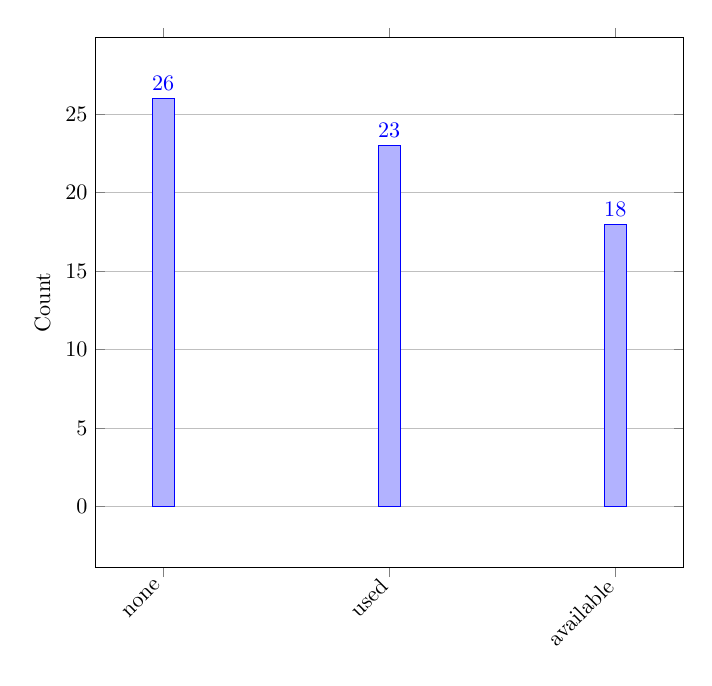
\begin{tikzpicture}[scale=.8]
\begin{axis}[ ybar, ymajorgrids, enlargelimits=0.15, legend style={at={(0.5,-0.15)}, anchor=north,legend columns=-1},
    width=.90\linewidth,height=10cm,
    nodes near coords, %nodes near coords align=below,
    ylabel={Count}, ymin=0,
    x tick label style={rotate=45,anchor=east},
    xtick={1,2,3},
    xticklabels={none,used,available
}
    %xlabel={Tool Prototype}    
    ]
  \addplot coordinates { (1,26)  (2,23)  (3,18)   };
\end{axis}
\end{tikzpicture}
\end{center}
%\caption{Histogramm f\"ur Tool Prototype (67)}
%\label{fig:histo_toolprototype}
%\end{figure}


%\subsection{Histogramm f\"ur Input Data (70)}
%\begin{figure}
\begin{center}
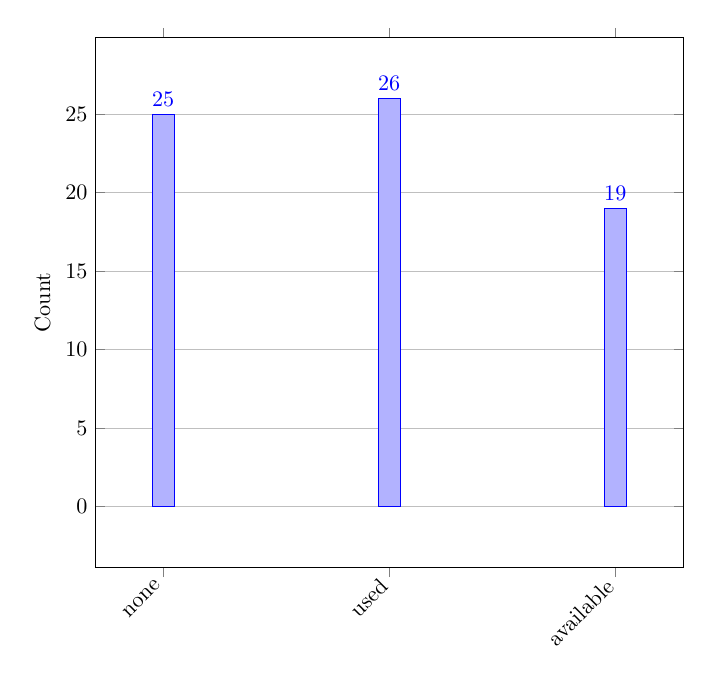
\begin{tikzpicture}[scale=.8]
\begin{axis}[ ybar, ymajorgrids, enlargelimits=0.15, legend style={at={(0.5,-0.15)}, anchor=north,legend columns=-1},
    width=.90\linewidth,height=10cm,
    nodes near coords, %nodes near coords align=below,
    ylabel={Count}, ymin=0,
    x tick label style={rotate=45,anchor=east},
    xtick={1,2,3},
    xticklabels={none,used,available
}
    %xlabel={Input Data}    
    ]
  \addplot coordinates { (1,25)  (2,26)  (3,19)   };
\end{axis}
\end{tikzpicture}
\end{center}
%\caption{Histogramm f\"ur Input Data (70)}
%\label{fig:histo_inputdata}
%\end{figure}


%\subsection{Pie chart for Tool Prototype (67)}
%\begin{figure}
\begin{center}
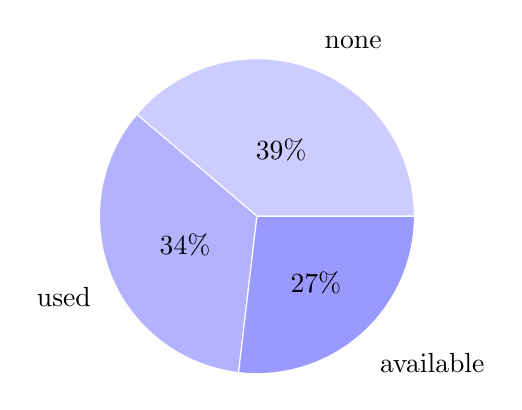
\begin{tikzpicture}[scale=2]
\pgfmathsetcounter{pief}{0}
\foreach \p/\q/\t/\c in {39/26/none/blue!20, 34/23/used/blue!30, 27/18/available/blue!40}
  {
    \setcounter{piee}{\value{pief}}
    \addtocounter{pief}{\q}
    \slice{\thepiee/67*360}
          {\thepief/67*360}
          {\p\%}{\t}{\c}
  }
\end{tikzpicture}

\textbf{Pie chart for Tool Prototype (67)}
\end{center}
%\caption{Pie chart for Tool Prototype (67)}
%\label{fig:pie_toolprototype}
%\end{figure}


%\subsection{Pie chart for Input Data (70)}
%\begin{figure}
\begin{center}
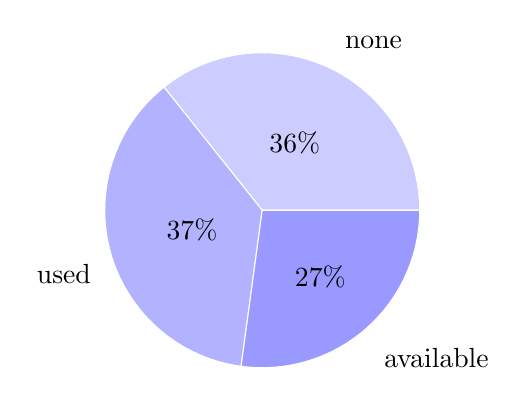
\begin{tikzpicture}[scale=2]
\pgfmathsetcounter{pief}{0}
\foreach \p/\q/\t/\c in {36/25/none/blue!20, 37/26/used/blue!30, 27/19/available/blue!40}
  {
    \setcounter{piee}{\value{pief}}
    \addtocounter{pief}{\q}
    \slice{\thepiee/70*360}
          {\thepief/70*360}
          {\p\%}{\t}{\c}
  }
\end{tikzpicture}

\textbf{Pie chart for Input Data (70)}
\end{center}
%\caption{Pie chart for Input Data (70)}
%\label{fig:pie_inputdata}
%\end{figure}


%\subsection{Pie chart for Replication Package (67)}
%\begin{figure}
\begin{center}
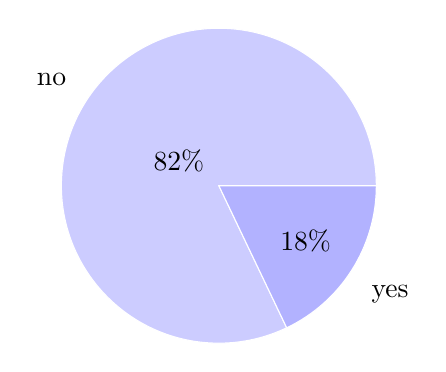
\begin{tikzpicture}[scale=2]
\pgfmathsetcounter{pief}{0}
\foreach \p/\q/\t/\c in {82/55/no/blue!20, 18/12/yes/blue!30}
  {
    \setcounter{piee}{\value{pief}}
    \addtocounter{pief}{\q}
    \slice{\thepiee/67*360}
          {\thepief/67*360}
          {\p\%}{\t}{\c}
  }
\end{tikzpicture}

\textbf{Pie chart for Replication Package (67)}
\end{center}
%\caption{Pie chart for Replication Package (67)}
%\label{fig:pie_replicationpackage}
%\end{figure}


%\subsection{Histogram von Year je Replication Package}
%\begin{figure}
\begin{center}
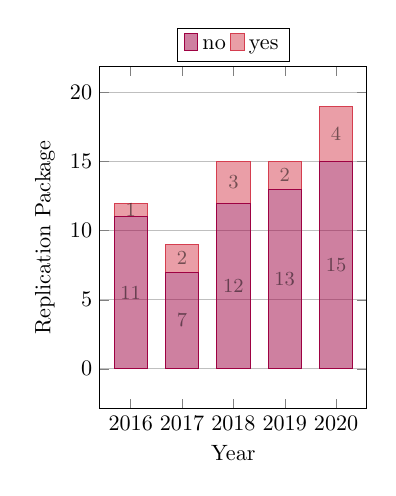
\begin{tikzpicture}[scale=0.8]
\
\begin{axis}[ width=.48\linewidth,height=7cm, ybar stacked,
    cycle multi list=Spectral,
    every axis plot/.append style={draw, fill, fill opacity=0.5},
    enlargelimits=0.15, 
    bar width=1.5em,
    nodes near coords, %nodes near coords align=below,
    nodes near coords style={color=black,font=\small},
    legend style={at={(0.5,1.115)}, anchor=north,legend columns=3},
    legend cell align={left},
    ylabel={Replication Package},ymajorgrids,ymin=0,
    %x tick label style={rotate=45,anchor=east},
    ymin=0,
    xtick={1,2,3,4,5}, xticklabels={2016,2017,2018,2019,2020},
    xlabel={Year}    
   ]
\addplot coordinates { (1,11)  (2,7)  (3,12)  (4,13)  (5,15)  };
\addplot coordinates { (1,1)  (2,2)  (3,3)  (4,2)  (5,4)  };

\legend{no,yes}
\end{axis}
\end{tikzpicture}
\end{center}
%\caption{Histogram von Year je Replication Package}
%\label{fig:chisto_year_replicationpackage}
%\end{figure}


%\subsection{Histogram von Year je Tool Prototype}
%\begin{figure}
\begin{center}
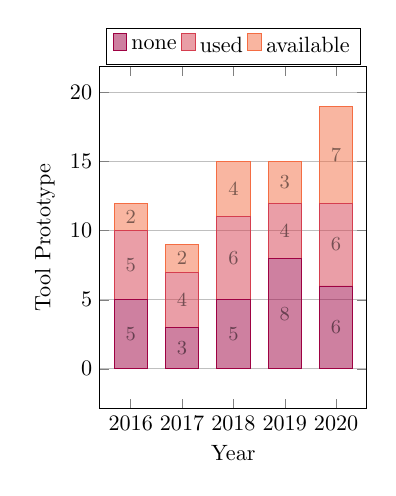
\begin{tikzpicture}[scale=0.8]
\
\begin{axis}[ width=.48\linewidth,height=7cm, ybar stacked,
    cycle multi list=Spectral,
    every axis plot/.append style={draw, fill, fill opacity=0.5},
    enlargelimits=0.15, 
    bar width=1.5em,
    nodes near coords, %nodes near coords align=below,
    nodes near coords style={color=black,font=\small},
    legend style={at={(0.5,1.115)}, anchor=north,legend columns=3},
    legend cell align={left},
    ylabel={Tool Prototype},ymajorgrids,ymin=0,
    %x tick label style={rotate=45,anchor=east},
    ymin=0,
    xtick={1,2,3,4,5}, xticklabels={2016,2017,2018,2019,2020},
    xlabel={Year}    
   ]
\addplot coordinates { (1,5)  (2,3)  (3,5)  (4,8)  (5,6)  };
\addplot coordinates { (1,5)  (2,4)  (3,6)  (4,4)  (5,6)  };
\addplot coordinates { (1,2)  (2,2)  (3,4)  (4,3)  (5,7)  };

\legend{none,used,available}
\end{axis}
\end{tikzpicture}
\end{center}
%\caption{Histogram von Year je Tool Prototype}
%\label{fig:chisto_year_toolprototype}
%\end{figure}


%\subsection{Histogram von Year je Input Data}
%\begin{figure}
\begin{center}
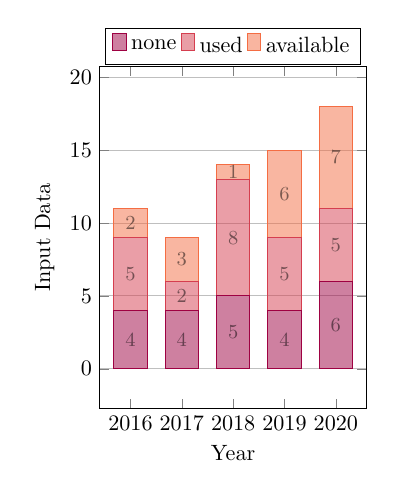
\begin{tikzpicture}[scale=0.8]
\
\begin{axis}[ width=.48\linewidth,height=7cm, ybar stacked,
    cycle multi list=Spectral,
    every axis plot/.append style={draw, fill, fill opacity=0.5},
    enlargelimits=0.15, 
    bar width=1.5em,
    nodes near coords, %nodes near coords align=below,
    nodes near coords style={color=black,font=\small},
    legend style={at={(0.5,1.115)}, anchor=north,legend columns=3},
    legend cell align={left},
    ylabel={Input Data},ymajorgrids,ymin=0,
    %x tick label style={rotate=45,anchor=east},
    ymin=0,
    xtick={1,2,3,4,5}, xticklabels={2016,2017,2018,2019,2020},
    xlabel={Year}    
   ]
\addplot coordinates { (1,4)  (2,4)  (3,5)  (4,4)  (5,6)  };
\addplot coordinates { (1,5)  (2,2)  (3,8)  (4,5)  (5,5)  };
\addplot coordinates { (1,2)  (2,3)  (3,1)  (4,6)  (5,7)  };

\legend{none,used,available}
\end{axis}
\end{tikzpicture}
\end{center}
%\caption{Histogram von Year je Input Data}
%\label{fig:chisto_year_inputdata}
%\end{figure}



\section{Threats to Validity}

%\subsection{Histogramm f\"ur Threats to Validity (167)}
%\begin{figure}
\begin{center}
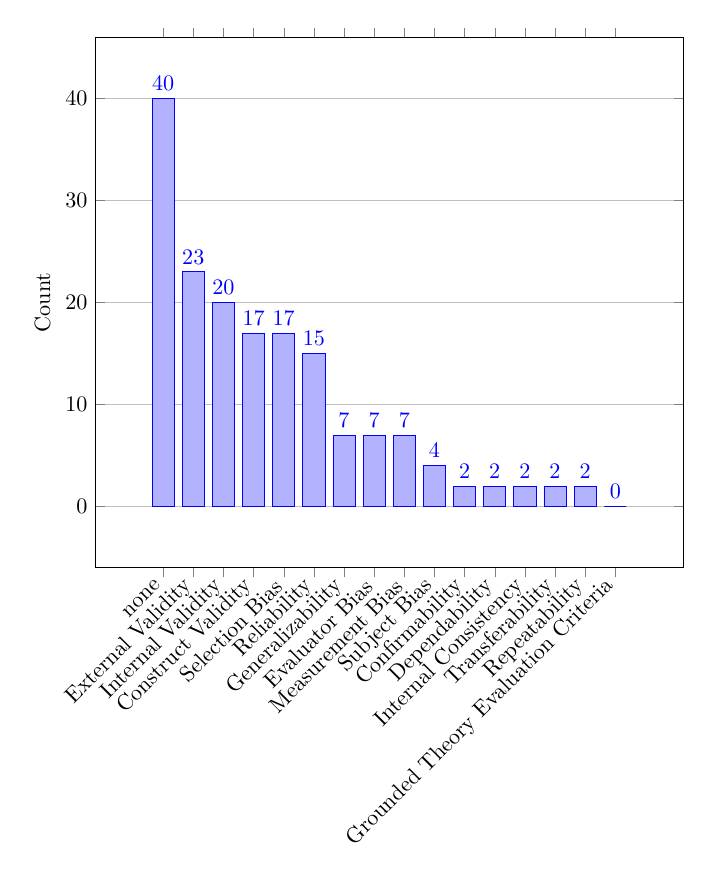
\begin{tikzpicture}[scale=.8]
\begin{axis}[ ybar, ymajorgrids, enlargelimits=0.15, legend style={at={(0.5,-0.15)}, anchor=north,legend columns=-1},
    width=.90\linewidth,height=10cm,
    nodes near coords, %nodes near coords align=below,
    ylabel={Count}, ymin=0,
    x tick label style={rotate=45,anchor=east},
    xtick={1,2,3,4,5,6,7,8,9,10,11,12,13,14,15,16},
    xticklabels={none, External Validity, Internal Validity, Construct Validity, Selection Bias, Reliability, Generalizability, Evaluator Bias, Measurement Bias, Subject Bias, Confirmability, Dependability, Internal Consistency ,Transferability, Repeatability, Grounded Theory Evaluation Criteria
}
    %xlabel={Threats to Validity}    
    ]
  \addplot coordinates { (1,40)  (2,23)  (3,20)  (4,17)  (5,17)  (6,15)  (7,7)  (8,7)  (9,7)  (10,4)  (11,2)  (12,2)  (13,2)  (14,2)  (15,2)  (16,0)   };
\end{axis}
\end{tikzpicture}
\end{center}
%\caption{Histogramm f\"ur Threats to Validity (167)}
%\label{fig:histo_threatstovalidity}
%\end{figure}


%\subsection{Histogramm f\"ur Year (71)}
%\begin{figure}
\begin{center}
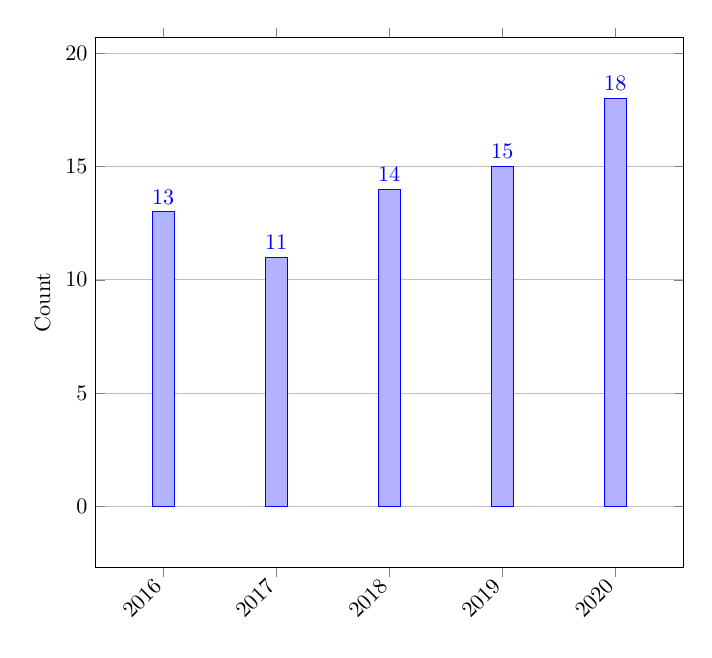
\begin{tikzpicture}[scale=.8]
\begin{axis}[ ybar, ymajorgrids, enlargelimits=0.15, legend style={at={(0.5,-0.15)}, anchor=north,legend columns=-1},
    width=.90\linewidth,height=10cm,
    nodes near coords, %nodes near coords align=below,
    ylabel={Count},ymin=0,
    x tick label style={rotate=45,anchor=east},
    xtick={1,2,3,4,5},
    xticklabels={2016,2017,2018,2019,2020
}
    %xlabel={Year}    
    ]
  \addplot coordinates { (1,13)  (2,11)  (3,14)  (4,15)  (5,18)   };
\end{axis}
\end{tikzpicture}
\end{center}
%\caption{Histogramm f\"ur Year (71)}
%\label{fig:histo_year}
%\end{figure}


\input{figs/chisto_year_threatstovalidity}

\section{Kinds vs. Evaluation Methods}

%\subsection{Histogramm f\"ur Industry Paper (67)}
%\begin{figure}
\begin{center}
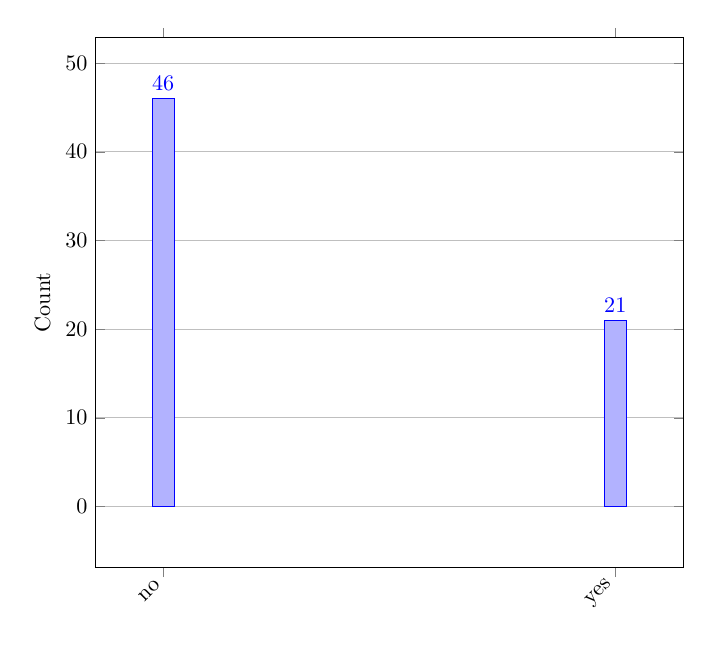
\begin{tikzpicture}[scale=.8]
\begin{axis}[ ybar, ymajorgrids, enlargelimits=0.15, legend style={at={(0.5,-0.15)}, anchor=north,legend columns=-1},
    width=.90\linewidth,height=10cm,
    nodes near coords, %nodes near coords align=below,
    ylabel={Count},ymin=0,
    x tick label style={rotate=45,anchor=east},
    xtick={1,2},
    xticklabels={no,yes
}
    %xlabel={Industry Paper}    
    ]
  \addplot coordinates { (1,46)  (2,21)   };
\end{axis}
\end{tikzpicture}
\end{center}
%\caption{Histogramm f\"ur Industry Paper (67)}
%\label{fig:histo_industrypaper}
%\end{figure}


%\subsection{Histogramm f\"ur Evaluation Methods (87)}
%\begin{figure}
\begin{center}
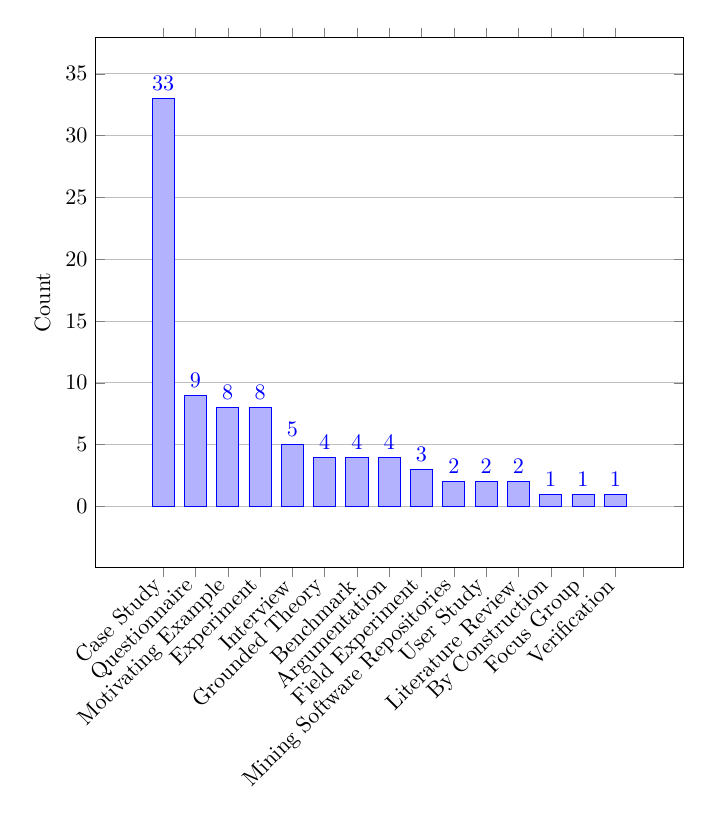
\begin{tikzpicture}[scale=.8]
\begin{axis}[ ybar, ymajorgrids, enlargelimits=0.15, legend style={at={(0.5,-0.15)}, anchor=north,legend columns=-1},
    width=.90\linewidth,height=10cm,
    nodes near coords, %nodes near coords align=below,
    ylabel={Count},ymin=0,
    x tick label style={rotate=45,anchor=east},
    xtick={1,2,3,4,5,6,7,8,9,10,11,12,13,14,15},
    xticklabels={Case Study,Questionnaire,Motivating Example,Experiment,Interview,Grounded Theory,Benchmark,Argumentation,Field Experiment,Mining Software Repositories,User Study,Literature Review,By Construction,Focus Group,Verification
}
    %xlabel={Evaluation Methods}    
    ]
  \addplot coordinates { (1,33)  (2,9)  (3,8)  (4,8)  (5,5)  (6,4)  (7,4)  (8,4)  (9,3)  (10,2)  (11,2)  (12,2)  (13,1)  (14,1)  (15,1)   };
\end{axis}
\end{tikzpicture}
\end{center}
%\caption{Histogramm f\"ur Evaluation Methods (87)}
%\label{fig:histo_evaluationmethods}
%\end{figure}


%\subsection{Histogram von Industry Paper je Evaluation Methods}
%\begin{figure}
\begin{center}
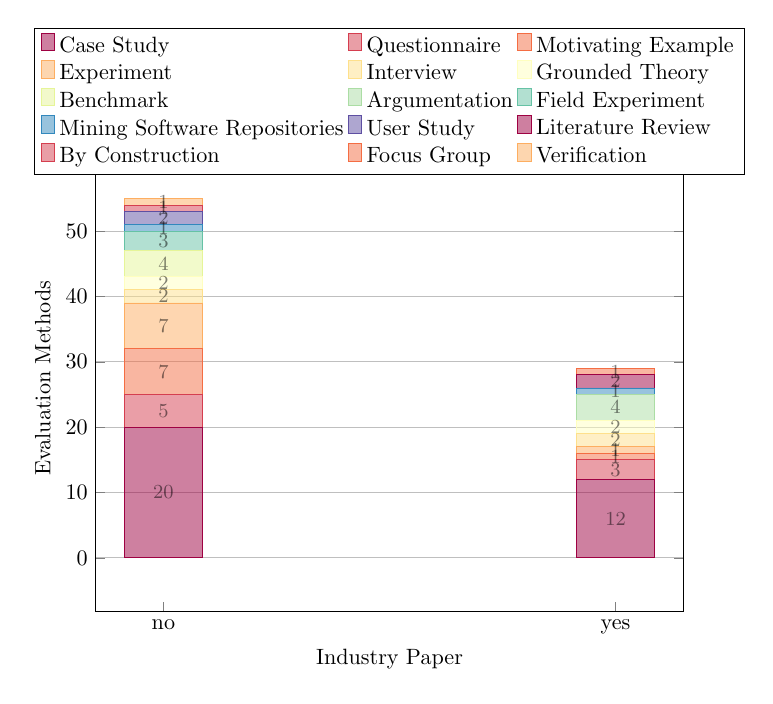
\begin{tikzpicture}[scale=0.8]
\
\begin{axis}[ width=.9\linewidth,height=9cm, ybar stacked,
    cycle multi list=Spectral,
    every axis plot/.append style={draw, fill, fill opacity=0.5},
    enlargelimits=0.15, 
    bar width=3.5em,
    nodes near coords, %nodes near coords align=below,
    nodes near coords style={color=black,font=\small},
    legend style={at={(0.5,1.25)}, anchor=north,legend columns=3},
    legend cell align={left},
    ylabel={Evaluation Methods},ymajorgrids,ymin=0,
    %x tick label style={rotate=45,anchor=east},
    xtick={1,2}, xticklabels={no,yes},
    xlabel={Industry Paper}    
   ]
\addplot coordinates { (1,20)  (2,12)  };
\addplot coordinates { (1,5)  (2,3)  };
\addplot coordinates { (1,7)  (2,1)  };
\addplot coordinates { (1,7)  (2,1)  };
\addplot coordinates { (1,2)  (2,2)  };
\addplot coordinates { (1,2)  (2,2)  };
\addplot coordinates { (1,4)  (2,0)  };
\addplot coordinates { (1,0)  (2,4)  };
\addplot coordinates { (1,3)  (2,0)  };
\addplot coordinates { (1,1)  (2,1)  };
\addplot coordinates { (1,2)  (2,0)  };
\addplot coordinates { (1,0)  (2,2)  };
\addplot coordinates { (1,1)  (2,0)  };
\addplot coordinates { (1,0)  (2,1)  };
\addplot coordinates { (1,1)  (2,0)  };

\legend{Case Study,Questionnaire,Motivating Example,Experiment,Interview,Grounded Theory,Benchmark,Argumentation,Field Experiment,Mining Software Repositories,User Study,Literature Review,By Construction,Focus Group,Verification}
\end{axis}
\end{tikzpicture}
\end{center}
%\caption{Histogram von Industry Paper je Evaluation Methods}
%\label{fig:chisto_industrypaper_evaluationmethods}
%\end{figure}


%\subsection{Portfolio f\"ur Evaluation Methods und Industry Paper (Gr\"o\ss{}e entspricht der Anzahl)}
%\begin{figure}
\begin{center}
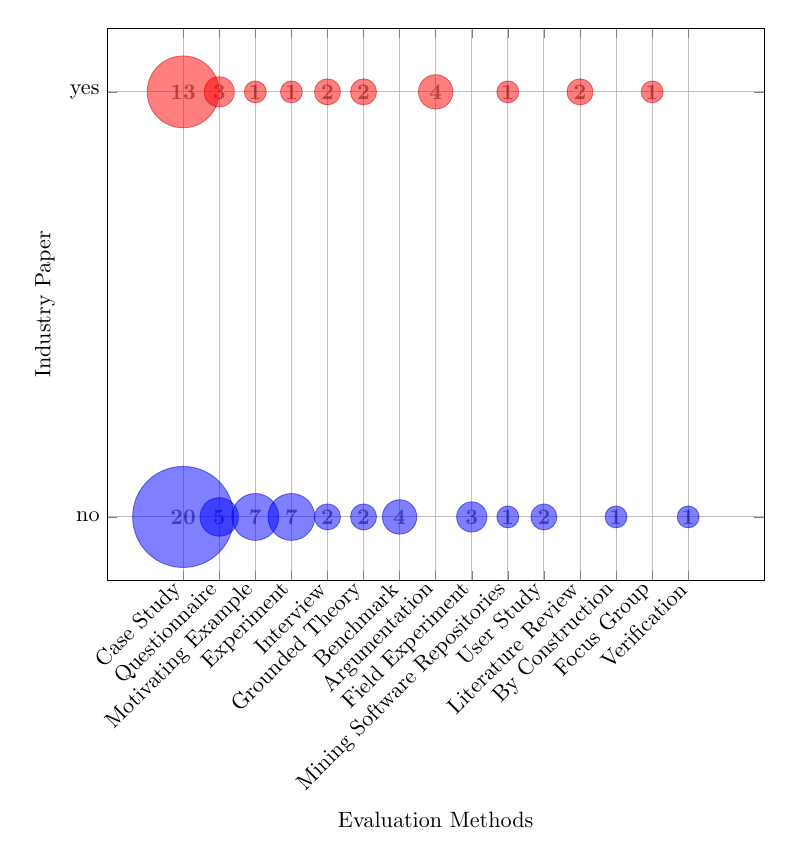
\begin{tikzpicture}[scale=.8]
\begin{axis}[scatter,
    width=.99\linewidth,
    cycle multi list=Spectral,
    every axis plot/.append style={draw, fill, fill opacity=0.5},
    scatter src=y,
    nodes near coords style={color=black,font=\small},
    enlargelimits=0.15,
    x tick label style={rotate=45,anchor=east},
    xtick={0,1,2,3,4,5,6,7,8,9,10,11,12,13,14}, xticklabels={Case Study,Questionnaire,Motivating Example,Experiment,Interview,Grounded Theory,Benchmark,Argumentation,Field Experiment,Mining Software Repositories,User Study,Literature Review,By Construction,Focus Group,Verification},
    xlabel={Evaluation Methods},
    ytick={0,1}, yticklabels={no,yes},
    ylabel={Industry Paper},
    grid=both
]

\addplot[mark size=22.824,opacity=0.5,text=black] coordinates { (0,0) } node[text=black,font=\bfseries] {20};
\addplot[mark size=16.235,opacity=0.5,text=black] coordinates { (0,1) } node[text=black,font=\bfseries] {13};
\addplot[mark size=8.706,opacity=0.5,text=black] coordinates { (1,0) } node[text=black,font=\bfseries] {5};
\addplot[mark size=6.824,opacity=0.5,text=black] coordinates { (1,1) } node[text=black,font=\bfseries] {3};
\addplot[mark size=10.588,opacity=0.5,text=black] coordinates { (2,0) } node[text=black,font=\bfseries] {7};
\addplot[mark size=4.941,opacity=0.5,text=black] coordinates { (2,1) } node[text=black,font=\bfseries] {1};
\addplot[mark size=10.588,opacity=0.5,text=black] coordinates { (3,0) } node[text=black,font=\bfseries] {7};
\addplot[mark size=4.941,opacity=0.5,text=black] coordinates { (3,1) } node[text=black,font=\bfseries] {1};
\addplot[mark size=5.882,opacity=0.5,text=black] coordinates { (4,0) } node[text=black,font=\bfseries] {2};
\addplot[mark size=5.882,opacity=0.5,text=black] coordinates { (4,1) } node[text=black,font=\bfseries] {2};
\addplot[mark size=5.882,opacity=0.5,text=black] coordinates { (5,0) } node[text=black,font=\bfseries] {2};
\addplot[mark size=5.882,opacity=0.5,text=black] coordinates { (5,1) } node[text=black,font=\bfseries] {2};
\addplot[mark size=7.765,opacity=0.5,text=black] coordinates { (6,0) } node[text=black,font=\bfseries] {4};
\addplot[mark size=7.765,opacity=0.5,text=black] coordinates { (7,1) } node[text=black,font=\bfseries] {4};
\addplot[mark size=6.824,opacity=0.5,text=black] coordinates { (8,0) } node[text=black,font=\bfseries] {3};
\addplot[mark size=4.941,opacity=0.5,text=black] coordinates { (9,0) } node[text=black,font=\bfseries] {1};
\addplot[mark size=4.941,opacity=0.5,text=black] coordinates { (9,1) } node[text=black,font=\bfseries] {1};
\addplot[mark size=5.882,opacity=0.5,text=black] coordinates { (10,0) } node[text=black,font=\bfseries] {2};
\addplot[mark size=5.882,opacity=0.5,text=black] coordinates { (11,1) } node[text=black,font=\bfseries] {2};
\addplot[mark size=4.941,opacity=0.5,text=black] coordinates { (12,0) } node[text=black,font=\bfseries] {1};
\addplot[mark size=4.941,opacity=0.5,text=black] coordinates { (13,1) } node[text=black,font=\bfseries] {1};
\addplot[mark size=4.941,opacity=0.5,text=black] coordinates { (14,0) } node[text=black,font=\bfseries] {1};


\end{axis}
\end{tikzpicture}
\end{center}
%\caption{Portfolio f\"ur Evaluation Methods und Industry Paper (Gr\"o\ss{}e entspricht der Anzahl)}\label{fig:port_evaluationmethods_industrypaper}
%\end{figure}


%\subsection{Portfolio f\"ur Industry Paper und Evaluation Methods (Gr\"o\ss{}e entspricht der Anzahl)}
%\begin{figure}
\begin{center}
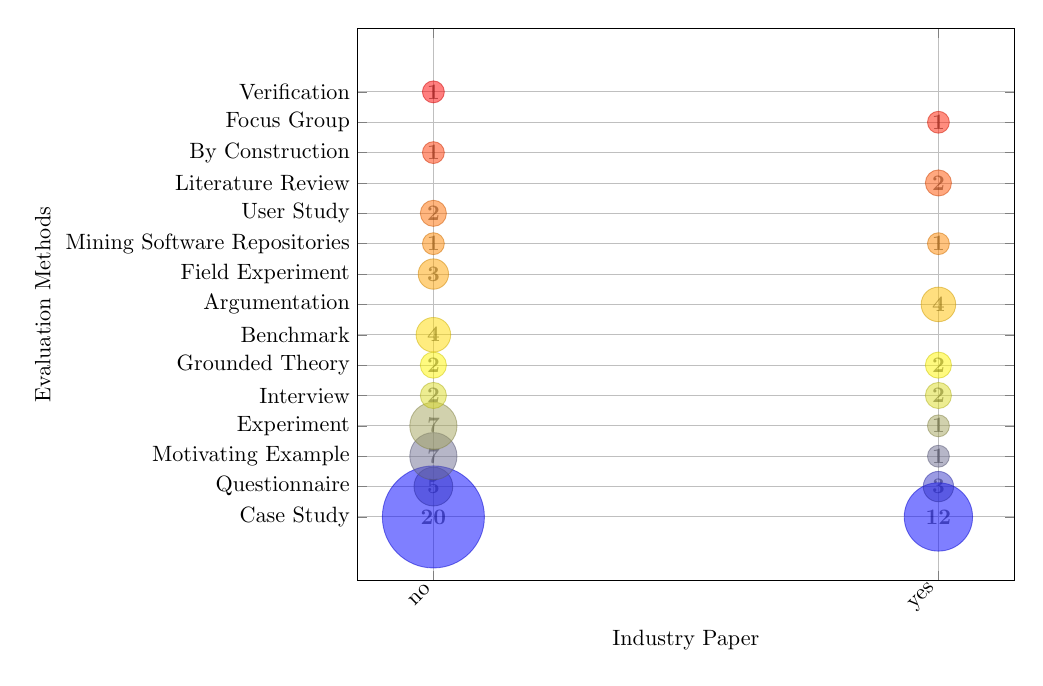
\begin{tikzpicture}[scale=.8]
\begin{axis}[scatter,
    width=.99\linewidth,
    cycle multi list=Spectral,
    every axis plot/.append style={draw, fill, fill opacity=0.5},
    scatter src=y,
    nodes near coords style={color=black,font=\small},
    enlargelimits=0.15,
    x tick label style={rotate=45,anchor=east},
    xtick={0,1}, xticklabels={no,yes},
    xlabel={Industry Paper},
    ytick={0,1,2,3,4,5,6,7,8,9,10,11,12,13,14}, yticklabels={Case Study,Questionnaire,Motivating Example,Experiment,Interview,Grounded Theory,Benchmark,Argumentation,Field Experiment,Mining Software Repositories,User Study,Literature Review,By Construction,Focus Group,Verification},
    ylabel={Evaluation Methods},
    grid=both
]

\addplot[mark size=23.048,opacity=0.5,text=black] coordinates { (0,0) } node[text=black,font=\bfseries] {20};
\addplot[mark size=8.762,opacity=0.5,text=black] coordinates { (0,1) } node[text=black,font=\bfseries] {5};
\addplot[mark size=10.667,opacity=0.5,text=black] coordinates { (0,2) } node[text=black,font=\bfseries] {7};
\addplot[mark size=10.667,opacity=0.5,text=black] coordinates { (0,3) } node[text=black,font=\bfseries] {7};
\addplot[mark size=5.905,opacity=0.5,text=black] coordinates { (0,4) } node[text=black,font=\bfseries] {2};
\addplot[mark size=5.905,opacity=0.5,text=black] coordinates { (0,5) } node[text=black,font=\bfseries] {2};
\addplot[mark size=7.810,opacity=0.5,text=black] coordinates { (0,6) } node[text=black,font=\bfseries] {4};
\addplot[mark size=6.857,opacity=0.5,text=black] coordinates { (0,8) } node[text=black,font=\bfseries] {3};
\addplot[mark size=4.952,opacity=0.5,text=black] coordinates { (0,9) } node[text=black,font=\bfseries] {1};
\addplot[mark size=5.905,opacity=0.5,text=black] coordinates { (0,10) } node[text=black,font=\bfseries] {2};
\addplot[mark size=4.952,opacity=0.5,text=black] coordinates { (0,12) } node[text=black,font=\bfseries] {1};
\addplot[mark size=4.952,opacity=0.5,text=black] coordinates { (0,14) } node[text=black,font=\bfseries] {1};
\addplot[mark size=15.429,opacity=0.5,text=black] coordinates { (1,0) } node[text=black,font=\bfseries] {12};
\addplot[mark size=6.857,opacity=0.5,text=black] coordinates { (1,1) } node[text=black,font=\bfseries] {3};
\addplot[mark size=4.952,opacity=0.5,text=black] coordinates { (1,2) } node[text=black,font=\bfseries] {1};
\addplot[mark size=4.952,opacity=0.5,text=black] coordinates { (1,3) } node[text=black,font=\bfseries] {1};
\addplot[mark size=5.905,opacity=0.5,text=black] coordinates { (1,4) } node[text=black,font=\bfseries] {2};
\addplot[mark size=5.905,opacity=0.5,text=black] coordinates { (1,5) } node[text=black,font=\bfseries] {2};
\addplot[mark size=7.810,opacity=0.5,text=black] coordinates { (1,7) } node[text=black,font=\bfseries] {4};
\addplot[mark size=4.952,opacity=0.5,text=black] coordinates { (1,9) } node[text=black,font=\bfseries] {1};
\addplot[mark size=5.905,opacity=0.5,text=black] coordinates { (1,11) } node[text=black,font=\bfseries] {2};
\addplot[mark size=4.952,opacity=0.5,text=black] coordinates { (1,13) } node[text=black,font=\bfseries] {1};


\end{axis}
\end{tikzpicture}
\end{center}
%\caption{Portfolio f\"ur Industry Paper und Evaluation Methods (Gr\"o\ss{}e entspricht der Anzahl)}\label{fig:port_industrypaper_evaluationmethods}
%\end{figure}



\section{Research Object vs. Property}

%\subsection{Histogramm f\"ur Research Object (75)}
%\begin{figure}
\begin{center}
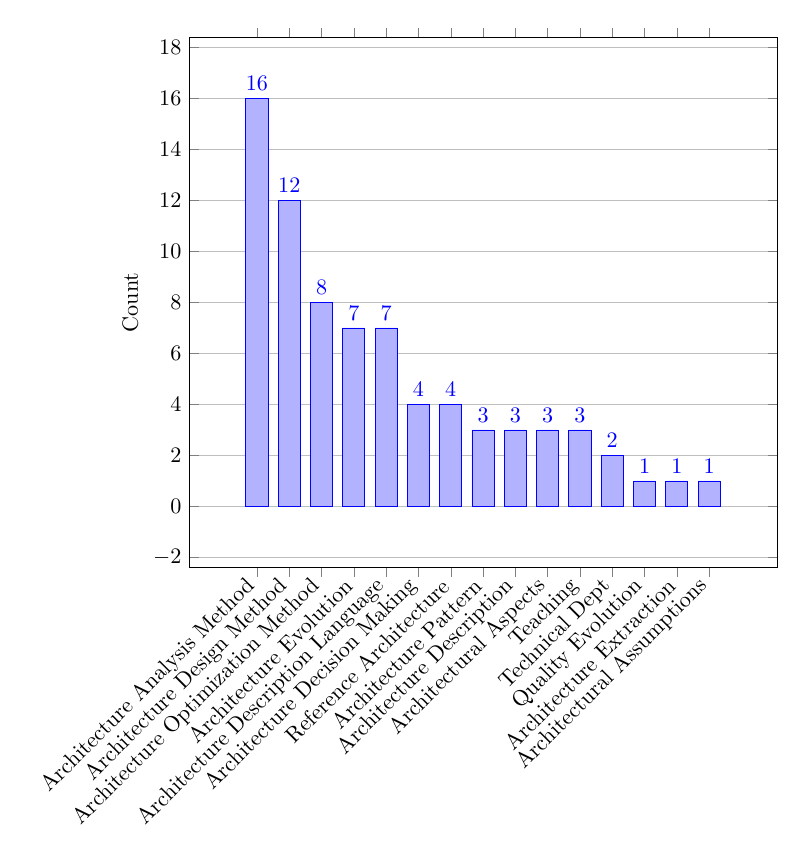
\begin{tikzpicture}[scale=.8]
\begin{axis}[ ybar, ymajorgrids, enlargelimits=0.15, legend style={at={(0.5,-0.15)}, anchor=north,legend columns=-1},
    width=.90\linewidth,height=10cm,
    nodes near coords, %nodes near coords align=below,
    ylabel={Count}, ymin=0,
    x tick label style={rotate=45,anchor=east},
    xtick={1,2,3,4,5,6,7,8,9,10,11,12,13,14,15},
    xticklabels={Architecture Analysis Method,Architecture Design Method,Architecture Optimization Method,Architecture Evolution,Architecture Description Language,Architecture Decision Making,Reference Architecture,Architecture Pattern,Architecture Description,Architectural Aspects,Teaching,Technical Dept,Quality Evolution,Architecture Extraction,Architectural Assumptions
}
    %xlabel={Research Object}    
    ]
  \addplot coordinates { (1,16)  (2,12)  (3,8)  (4,7)  (5,7)  (6,4)  (7,4)  (8,3)  (9,3)  (10,3)  (11,3)  (12,2)  (13,1)  (14,1)  (15,1)   };
\end{axis}
\end{tikzpicture}
\end{center}
%\caption{Histogramm f\"ur Research Object (75)}
%\label{fig:histo_researchobject}
%\end{figure}


%\subsection{Histogramm f\"ur Property Instance (126)}
%\begin{figure}
\begin{center}
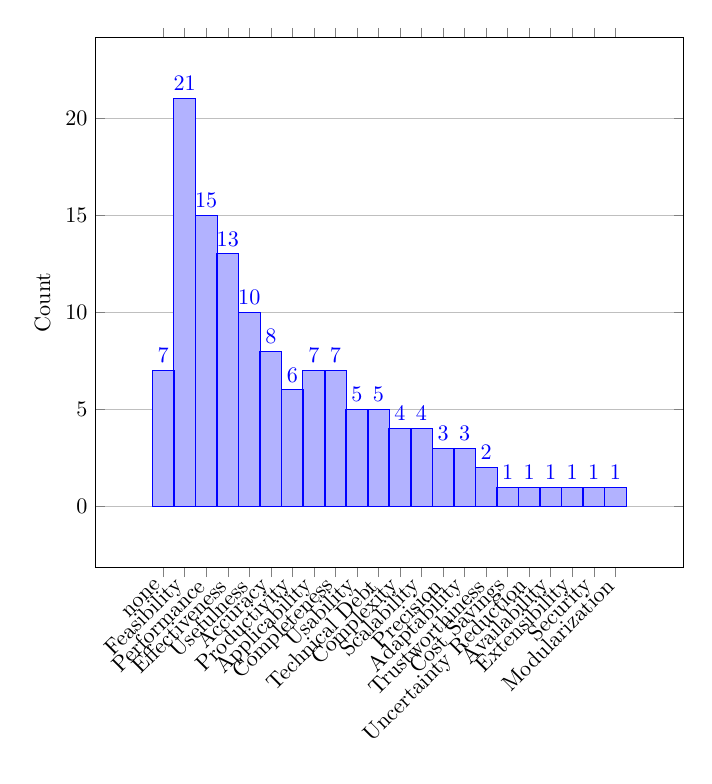
\begin{tikzpicture}[scale=.8]
\begin{axis}[ ybar, ymajorgrids, enlargelimits=0.15, legend style={at={(0.5,-0.15)}, anchor=north,legend columns=-1},
    width=.90\linewidth,height=10cm,
    nodes near coords, %nodes near coords align=below,
    ylabel={Count}, ymin=0,
    x tick label style={rotate=45,anchor=east},
    xtick={1,2,3,4,5,6,7,8,9,10,11,12,13,14,15,16,17,18,19,20,21,22},
    xticklabels={ none, Feasibility, Performance, Effectiveness, Usefulness, Accuracy,  Productivity, Applicability, Completeness, Usability, Technical Debt, Complexity, Scalability, Precision, Adaptability, Trustworthiness, Cost Savings, Uncertainty Reduction, Availability, Extensibility, Security, Modularization
}
    %xlabel={Property Instance}    
    ]
  \addplot coordinates { (1,7)  (2,21)  (3,15)  (4,13)  (5,10)  (6,8)  (7,6)  (8,7)  (9,7)  (10,5)  (11,5)  (12,4)  (13,4)  (14,3)  (15,3)  (16,2)  (17,1)  (18,1)  (19,1)  (20,1)  (21,1)  (22,1)   };
\end{axis}
\end{tikzpicture}
\end{center}
%\caption{Histogramm f\"ur Property Instance (126)}
%\label{fig:histo_propertyinstance}
%\end{figure}


%\subsection{Histogram von Year je Property Instance}
%\begin{figure}
\begin{center}
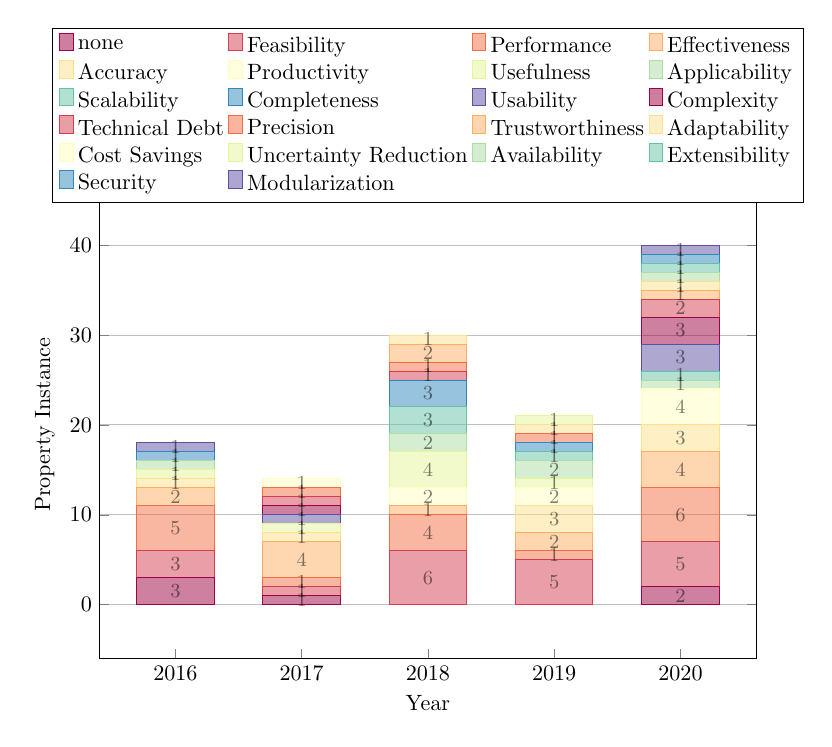
\begin{tikzpicture}[scale=0.8]
\
\begin{axis}[ width=.99\linewidth,height=9cm, ybar stacked,
    cycle multi list=Spectral,
    every axis plot/.append style={draw, fill, fill opacity=0.5},
    enlargelimits=0.15, 
    bar width=3.5em,
    nodes near coords, %nodes near coords align=below,
    nodes near coords style={color=black,font=\small},
    legend style={at={(0.5,1.35)}, anchor=north,legend columns=4},
    legend cell align={left},
    ylabel={Property Instance},ymajorgrids, ymin=0, 
    %x tick label style={rotate=45,anchor=east},
    xtick={1,2,3,4,5}, xticklabels={2016,2017,2018,2019,2020},
    xlabel={Year}    
   ]
\addplot coordinates { (1,3)  (2,1)  (3,0)  (4,0)  (5,2)  };
\addplot coordinates { (1,3)  (2,1)  (3,6)  (4,5)  (5,5)  };
\addplot coordinates { (1,5)  (2,1)  (3,4)  (4,1)  (5,6)  };
\addplot coordinates { (1,2)  (2,4)  (3,1)  (4,2)  (5,4)  };
\addplot coordinates { (1,1)  (2,1)  (3,0)  (4,3)  (5,3)  };
\addplot coordinates { (1,0)  (2,0)  (3,2)  (4,2)  (5,4)  };
\addplot coordinates { (1,1)  (2,1)  (3,4)  (4,1)  (5,0)  };
\addplot coordinates { (1,1)  (2,0)  (3,2)  (4,2)  (5,1)  };
\addplot coordinates { (1,0)  (2,0)  (3,3)  (4,1)  (5,1)  };
\addplot coordinates { (1,1)  (2,0)  (3,3)  (4,1)  (5,0)  };
\addplot coordinates { (1,1)  (2,1)  (3,0)  (4,0)  (5,3)  };
\addplot coordinates { (1,0)  (2,1)  (3,0)  (4,0)  (5,3)  };
\addplot coordinates { (1,0)  (2,1)  (3,1)  (4,0)  (5,2)  };
\addplot coordinates { (1,0)  (2,1)  (3,1)  (4,1)  (5,0)  };
\addplot coordinates { (1,0)  (2,0)  (3,2)  (4,0)  (5,1)  };
\addplot coordinates { (1,0)  (2,0)  (3,1)  (4,1)  (5,1)  };
\addplot coordinates { (1,0)  (2,1)  (3,0)  (4,0)  (5,0)  };
\addplot coordinates { (1,0)  (2,0)  (3,0)  (4,1)  (5,0)  };
\addplot coordinates { (1,0)  (2,0)  (3,0)  (4,0)  (5,1)  };
\addplot coordinates { (1,0)  (2,0)  (3,0)  (4,0)  (5,1)  };
\addplot coordinates { (1,0)  (2,0)  (3,0)  (4,0)  (5,1)  };
\addplot coordinates { (1,0)  (2,0)  (3,0)  (4,0)  (5,1)  };

\legend{none,Feasibility,Performance,Effectiveness,Accuracy,Productivity,Usefulness,Applicability,Scalability,Completeness,Usability,Complexity,Technical Debt,Precision,Trustworthiness,Adaptability,Cost Savings,Uncertainty Reduction,Availability,Extensibility,Security,Modularization}
\end{axis}
\end{tikzpicture}
\end{center}
%\caption{Histogram von Year je Property Instance}
%\label{fig:chisto_year_propertyinstance}
%\end{figure}


%\subsection{Portfolio f\"ur Research Object und Property Instance (Gr\"o\ss{}e entspricht der Anzahl)}
%\begin{figure}
\begin{center}
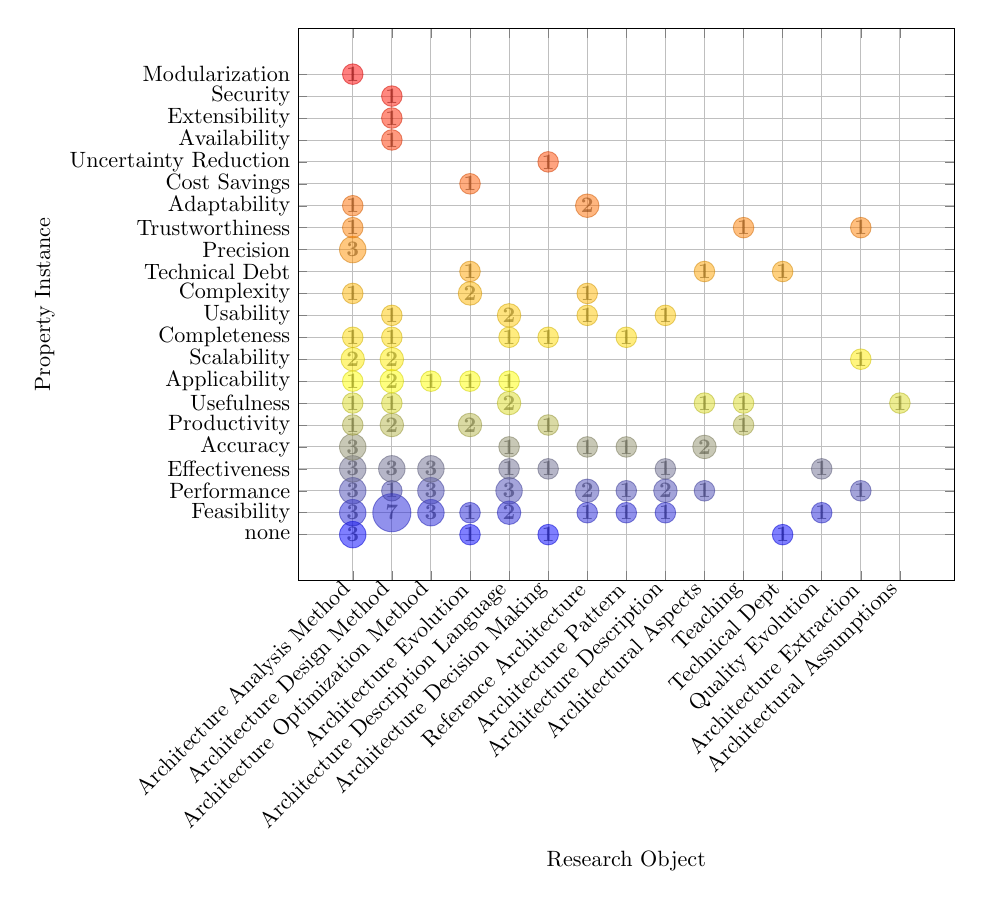
\begin{tikzpicture}[scale=.8]
\begin{axis}[scatter,
    width=.99\linewidth,
    cycle multi list=Spectral,
    every axis plot/.append style={draw, fill, fill opacity=0.5},
    scatter src=y,
    nodes near coords style={color=black,font=\small},
    %enlargelimits=0.15,
    x tick label style={rotate=45,anchor=east},
    xtick={0,1,2,3,4,5,6,7,8,9,10,11,12,13,14}, xticklabels={Architecture Analysis Method,Architecture Design Method,Architecture Optimization Method,Architecture Evolution,Architecture Description Language,Architecture Decision Making,Reference Architecture,Architecture Pattern,Architecture Description,Architectural Aspects,Teaching,Technical Dept,Quality Evolution,Architecture Extraction,Architectural Assumptions},
    xlabel={Research Object},
    ytick={0,1,2,3,4,5,6,7,8,9,10,11,12,13,14,15,16,17,18,19,20,21}, yticklabels={none,Feasibility,Performance,Effectiveness,Accuracy,Productivity,Usefulness,Applicability,Scalability,Completeness,Usability,Complexity,Technical Debt,Precision,Trustworthiness,Adaptability,Cost Savings,Uncertainty Reduction,Availability,Extensibility,Security,Modularization},
    ylabel={Property Instance},
    grid=both
]

\addplot[mark size=5.983,opacity=0.5,text=black] coordinates { (0,0) } node[text=black,font=\bfseries] {3};
\addplot[mark size=5.983,opacity=0.5,text=black] coordinates { (0,1) } node[text=black,font=\bfseries] {3};
\addplot[mark size=5.983,opacity=0.5,text=black] coordinates { (0,2) } node[text=black,font=\bfseries] {3};
\addplot[mark size=5.983,opacity=0.5,text=black] coordinates { (0,3) } node[text=black,font=\bfseries] {3};
\addplot[mark size=5.983,opacity=0.5,text=black] coordinates { (0,4) } node[text=black,font=\bfseries] {3};
\addplot[mark size=4.661,opacity=0.5,text=black] coordinates { (0,5) } node[text=black,font=\bfseries] {1};
\addplot[mark size=4.661,opacity=0.5,text=black] coordinates { (0,6) } node[text=black,font=\bfseries] {1};
\addplot[mark size=4.661,opacity=0.5,text=black] coordinates { (0,7) } node[text=black,font=\bfseries] {1};
\addplot[mark size=5.322,opacity=0.5,text=black] coordinates { (0,8) } node[text=black,font=\bfseries] {2};
\addplot[mark size=4.661,opacity=0.5,text=black] coordinates { (0,9) } node[text=black,font=\bfseries] {1};
\addplot[mark size=4.661,opacity=0.5,text=black] coordinates { (0,11) } node[text=black,font=\bfseries] {1};
\addplot[mark size=5.983,opacity=0.5,text=black] coordinates { (0,13) } node[text=black,font=\bfseries] {3};
\addplot[mark size=4.661,opacity=0.5,text=black] coordinates { (0,14) } node[text=black,font=\bfseries] {1};
\addplot[mark size=4.661,opacity=0.5,text=black] coordinates { (0,15) } node[text=black,font=\bfseries] {1};
\addplot[mark size=4.661,opacity=0.5,text=black] coordinates { (0,21) } node[text=black,font=\bfseries] {1};
\addplot[mark size=8.628,opacity=0.5,text=black] coordinates { (1,1) } node[text=black,font=\bfseries] {7};
\addplot[mark size=4.661,opacity=0.5,text=black] coordinates { (1,2) } node[text=black,font=\bfseries] {1};
\addplot[mark size=5.983,opacity=0.5,text=black] coordinates { (1,3) } node[text=black,font=\bfseries] {3};
\addplot[mark size=5.322,opacity=0.5,text=black] coordinates { (1,5) } node[text=black,font=\bfseries] {2};
\addplot[mark size=4.661,opacity=0.5,text=black] coordinates { (1,6) } node[text=black,font=\bfseries] {1};
\addplot[mark size=5.322,opacity=0.5,text=black] coordinates { (1,7) } node[text=black,font=\bfseries] {2};
\addplot[mark size=5.322,opacity=0.5,text=black] coordinates { (1,8) } node[text=black,font=\bfseries] {2};
\addplot[mark size=4.661,opacity=0.5,text=black] coordinates { (1,9) } node[text=black,font=\bfseries] {1};
\addplot[mark size=4.661,opacity=0.5,text=black] coordinates { (1,10) } node[text=black,font=\bfseries] {1};
\addplot[mark size=4.661,opacity=0.5,text=black] coordinates { (1,18) } node[text=black,font=\bfseries] {1};
\addplot[mark size=4.661,opacity=0.5,text=black] coordinates { (1,19) } node[text=black,font=\bfseries] {1};
\addplot[mark size=4.661,opacity=0.5,text=black] coordinates { (1,20) } node[text=black,font=\bfseries] {1};
\addplot[mark size=5.983,opacity=0.5,text=black] coordinates { (2,1) } node[text=black,font=\bfseries] {3};
\addplot[mark size=5.983,opacity=0.5,text=black] coordinates { (2,2) } node[text=black,font=\bfseries] {3};
\addplot[mark size=5.983,opacity=0.5,text=black] coordinates { (2,3) } node[text=black,font=\bfseries] {3};
\addplot[mark size=4.661,opacity=0.5,text=black] coordinates { (2,7) } node[text=black,font=\bfseries] {1};
\addplot[mark size=4.661,opacity=0.5,text=black] coordinates { (3,0) } node[text=black,font=\bfseries] {1};
\addplot[mark size=4.661,opacity=0.5,text=black] coordinates { (3,1) } node[text=black,font=\bfseries] {1};
\addplot[mark size=5.322,opacity=0.5,text=black] coordinates { (3,5) } node[text=black,font=\bfseries] {2};
\addplot[mark size=4.661,opacity=0.5,text=black] coordinates { (3,7) } node[text=black,font=\bfseries] {1};
\addplot[mark size=5.322,opacity=0.5,text=black] coordinates { (3,11) } node[text=black,font=\bfseries] {2};
\addplot[mark size=4.661,opacity=0.5,text=black] coordinates { (3,12) } node[text=black,font=\bfseries] {1};
\addplot[mark size=4.661,opacity=0.5,text=black] coordinates { (3,16) } node[text=black,font=\bfseries] {1};
\addplot[mark size=5.322,opacity=0.5,text=black] coordinates { (4,1) } node[text=black,font=\bfseries] {2};
\addplot[mark size=5.983,opacity=0.5,text=black] coordinates { (4,2) } node[text=black,font=\bfseries] {3};
\addplot[mark size=4.661,opacity=0.5,text=black] coordinates { (4,3) } node[text=black,font=\bfseries] {1};
\addplot[mark size=4.661,opacity=0.5,text=black] coordinates { (4,4) } node[text=black,font=\bfseries] {1};
\addplot[mark size=5.322,opacity=0.5,text=black] coordinates { (4,6) } node[text=black,font=\bfseries] {2};
\addplot[mark size=4.661,opacity=0.5,text=black] coordinates { (4,7) } node[text=black,font=\bfseries] {1};
\addplot[mark size=4.661,opacity=0.5,text=black] coordinates { (4,9) } node[text=black,font=\bfseries] {1};
\addplot[mark size=5.322,opacity=0.5,text=black] coordinates { (4,10) } node[text=black,font=\bfseries] {2};
\addplot[mark size=4.661,opacity=0.5,text=black] coordinates { (5,0) } node[text=black,font=\bfseries] {1};
\addplot[mark size=4.661,opacity=0.5,text=black] coordinates { (5,3) } node[text=black,font=\bfseries] {1};
\addplot[mark size=4.661,opacity=0.5,text=black] coordinates { (5,5) } node[text=black,font=\bfseries] {1};
\addplot[mark size=4.661,opacity=0.5,text=black] coordinates { (5,9) } node[text=black,font=\bfseries] {1};
\addplot[mark size=4.661,opacity=0.5,text=black] coordinates { (5,17) } node[text=black,font=\bfseries] {1};
\addplot[mark size=4.661,opacity=0.5,text=black] coordinates { (6,1) } node[text=black,font=\bfseries] {1};
\addplot[mark size=5.322,opacity=0.5,text=black] coordinates { (6,2) } node[text=black,font=\bfseries] {2};
\addplot[mark size=4.661,opacity=0.5,text=black] coordinates { (6,4) } node[text=black,font=\bfseries] {1};
\addplot[mark size=4.661,opacity=0.5,text=black] coordinates { (6,10) } node[text=black,font=\bfseries] {1};
\addplot[mark size=4.661,opacity=0.5,text=black] coordinates { (6,11) } node[text=black,font=\bfseries] {1};
\addplot[mark size=5.322,opacity=0.5,text=black] coordinates { (6,15) } node[text=black,font=\bfseries] {2};
\addplot[mark size=4.661,opacity=0.5,text=black] coordinates { (7,1) } node[text=black,font=\bfseries] {1};
\addplot[mark size=4.661,opacity=0.5,text=black] coordinates { (7,2) } node[text=black,font=\bfseries] {1};
\addplot[mark size=4.661,opacity=0.5,text=black] coordinates { (7,4) } node[text=black,font=\bfseries] {1};
\addplot[mark size=4.661,opacity=0.5,text=black] coordinates { (7,9) } node[text=black,font=\bfseries] {1};
\addplot[mark size=4.661,opacity=0.5,text=black] coordinates { (8,1) } node[text=black,font=\bfseries] {1};
\addplot[mark size=5.322,opacity=0.5,text=black] coordinates { (8,2) } node[text=black,font=\bfseries] {2};
\addplot[mark size=4.661,opacity=0.5,text=black] coordinates { (8,3) } node[text=black,font=\bfseries] {1};
\addplot[mark size=4.661,opacity=0.5,text=black] coordinates { (8,10) } node[text=black,font=\bfseries] {1};
\addplot[mark size=4.661,opacity=0.5,text=black] coordinates { (9,2) } node[text=black,font=\bfseries] {1};
\addplot[mark size=5.322,opacity=0.5,text=black] coordinates { (9,4) } node[text=black,font=\bfseries] {2};
\addplot[mark size=4.661,opacity=0.5,text=black] coordinates { (9,6) } node[text=black,font=\bfseries] {1};
\addplot[mark size=4.661,opacity=0.5,text=black] coordinates { (9,12) } node[text=black,font=\bfseries] {1};
\addplot[mark size=4.661,opacity=0.5,text=black] coordinates { (10,5) } node[text=black,font=\bfseries] {1};
\addplot[mark size=4.661,opacity=0.5,text=black] coordinates { (10,6) } node[text=black,font=\bfseries] {1};
\addplot[mark size=4.661,opacity=0.5,text=black] coordinates { (10,14) } node[text=black,font=\bfseries] {1};
\addplot[mark size=4.661,opacity=0.5,text=black] coordinates { (11,0) } node[text=black,font=\bfseries] {1};
\addplot[mark size=4.661,opacity=0.5,text=black] coordinates { (11,12) } node[text=black,font=\bfseries] {1};
\addplot[mark size=4.661,opacity=0.5,text=black] coordinates { (12,1) } node[text=black,font=\bfseries] {1};
\addplot[mark size=4.661,opacity=0.5,text=black] coordinates { (12,3) } node[text=black,font=\bfseries] {1};
\addplot[mark size=4.661,opacity=0.5,text=black] coordinates { (13,2) } node[text=black,font=\bfseries] {1};
\addplot[mark size=4.661,opacity=0.5,text=black] coordinates { (13,8) } node[text=black,font=\bfseries] {1};
\addplot[mark size=4.661,opacity=0.5,text=black] coordinates { (13,14) } node[text=black,font=\bfseries] {1};
\addplot[mark size=4.661,opacity=0.5,text=black] coordinates { (14,6) } node[text=black,font=\bfseries] {1};


\end{axis}
\end{tikzpicture}
\end{center}
%\caption{Portfolio f\"ur Research Object und Property Instance (Gr\"o\ss{}e entspricht der Anzahl)}\label{fig:port_researchobject_propertyinstance}
%\end{figure}


%\subsection{Portfolio f\"ur Property Instance und Research Object (Gr\"o\ss{}e entspricht der Anzahl)}
%\begin{figure}
\begin{center}
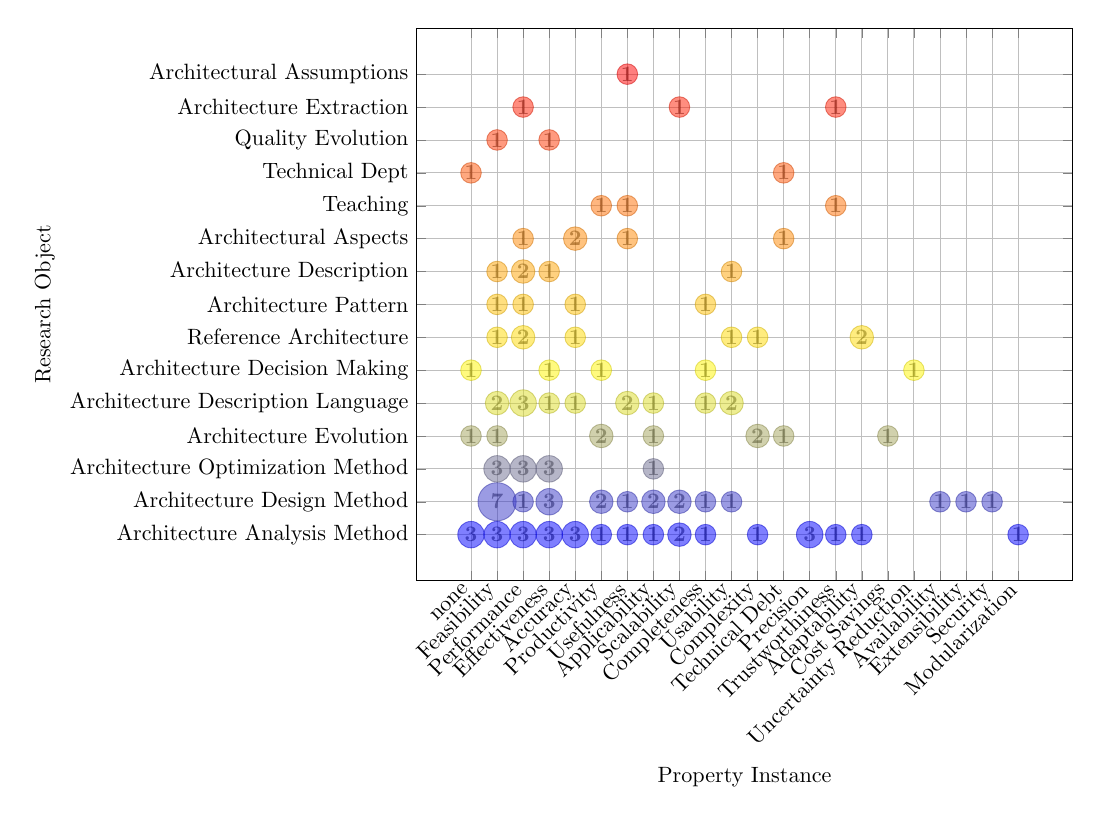
\begin{tikzpicture}[scale=.8]
\begin{axis}[scatter,
    width=.99\linewidth,
    cycle multi list=Spectral,
    every axis plot/.append style={draw, fill, fill opacity=0.5},
    scatter src=y,
    nodes near coords style={color=black,font=\small},
    %enlargelimits=0.15,
    x tick label style={rotate=45,anchor=east},
    xtick={0,1,2,3,4,5,6,7,8,9,10,11,12,13,14,15,16,17,18,19,20,21}, xticklabels={none,Feasibility,Performance,Effectiveness,Accuracy,Productivity,Usefulness,Applicability,Scalability,Completeness,Usability,Complexity,Technical Debt,Precision,Trustworthiness,Adaptability,Cost Savings,Uncertainty Reduction,Availability,Extensibility,Security,Modularization},
    xlabel={Property Instance},
    ytick={0,1,2,3,4,5,6,7,8,9,10,11,12,13,14}, yticklabels={Architecture Analysis Method,Architecture Design Method,Architecture Optimization Method,Architecture Evolution,Architecture Description Language,Architecture Decision Making,Reference Architecture,Architecture Pattern,Architecture Description,Architectural Aspects,Teaching,Technical Dept,Quality Evolution,Architecture Extraction,Architectural Assumptions},
    ylabel={Research Object},
    grid=both
]

\addplot[mark size=5.983,opacity=0.5,text=black] coordinates { (0,0) } node[text=black,font=\bfseries] {3};
\addplot[mark size=4.661,opacity=0.5,text=black] coordinates { (0,3) } node[text=black,font=\bfseries] {1};
\addplot[mark size=4.661,opacity=0.5,text=black] coordinates { (0,5) } node[text=black,font=\bfseries] {1};
\addplot[mark size=4.661,opacity=0.5,text=black] coordinates { (0,11) } node[text=black,font=\bfseries] {1};
\addplot[mark size=5.983,opacity=0.5,text=black] coordinates { (1,0) } node[text=black,font=\bfseries] {3};
\addplot[mark size=8.628,opacity=0.5,text=black] coordinates { (1,1) } node[text=black,font=\bfseries] {7};
\addplot[mark size=5.983,opacity=0.5,text=black] coordinates { (1,2) } node[text=black,font=\bfseries] {3};
\addplot[mark size=4.661,opacity=0.5,text=black] coordinates { (1,3) } node[text=black,font=\bfseries] {1};
\addplot[mark size=5.322,opacity=0.5,text=black] coordinates { (1,4) } node[text=black,font=\bfseries] {2};
\addplot[mark size=4.661,opacity=0.5,text=black] coordinates { (1,6) } node[text=black,font=\bfseries] {1};
\addplot[mark size=4.661,opacity=0.5,text=black] coordinates { (1,7) } node[text=black,font=\bfseries] {1};
\addplot[mark size=4.661,opacity=0.5,text=black] coordinates { (1,8) } node[text=black,font=\bfseries] {1};
\addplot[mark size=4.661,opacity=0.5,text=black] coordinates { (1,12) } node[text=black,font=\bfseries] {1};
\addplot[mark size=5.983,opacity=0.5,text=black] coordinates { (2,0) } node[text=black,font=\bfseries] {3};
\addplot[mark size=4.661,opacity=0.5,text=black] coordinates { (2,1) } node[text=black,font=\bfseries] {1};
\addplot[mark size=5.983,opacity=0.5,text=black] coordinates { (2,2) } node[text=black,font=\bfseries] {3};
\addplot[mark size=5.983,opacity=0.5,text=black] coordinates { (2,4) } node[text=black,font=\bfseries] {3};
\addplot[mark size=5.322,opacity=0.5,text=black] coordinates { (2,6) } node[text=black,font=\bfseries] {2};
\addplot[mark size=4.661,opacity=0.5,text=black] coordinates { (2,7) } node[text=black,font=\bfseries] {1};
\addplot[mark size=5.322,opacity=0.5,text=black] coordinates { (2,8) } node[text=black,font=\bfseries] {2};
\addplot[mark size=4.661,opacity=0.5,text=black] coordinates { (2,9) } node[text=black,font=\bfseries] {1};
\addplot[mark size=4.661,opacity=0.5,text=black] coordinates { (2,13) } node[text=black,font=\bfseries] {1};
\addplot[mark size=5.983,opacity=0.5,text=black] coordinates { (3,0) } node[text=black,font=\bfseries] {3};
\addplot[mark size=5.983,opacity=0.5,text=black] coordinates { (3,1) } node[text=black,font=\bfseries] {3};
\addplot[mark size=5.983,opacity=0.5,text=black] coordinates { (3,2) } node[text=black,font=\bfseries] {3};
\addplot[mark size=4.661,opacity=0.5,text=black] coordinates { (3,4) } node[text=black,font=\bfseries] {1};
\addplot[mark size=4.661,opacity=0.5,text=black] coordinates { (3,5) } node[text=black,font=\bfseries] {1};
\addplot[mark size=4.661,opacity=0.5,text=black] coordinates { (3,8) } node[text=black,font=\bfseries] {1};
\addplot[mark size=4.661,opacity=0.5,text=black] coordinates { (3,12) } node[text=black,font=\bfseries] {1};
\addplot[mark size=5.983,opacity=0.5,text=black] coordinates { (4,0) } node[text=black,font=\bfseries] {3};
\addplot[mark size=4.661,opacity=0.5,text=black] coordinates { (4,4) } node[text=black,font=\bfseries] {1};
\addplot[mark size=4.661,opacity=0.5,text=black] coordinates { (4,6) } node[text=black,font=\bfseries] {1};
\addplot[mark size=4.661,opacity=0.5,text=black] coordinates { (4,7) } node[text=black,font=\bfseries] {1};
\addplot[mark size=5.322,opacity=0.5,text=black] coordinates { (4,9) } node[text=black,font=\bfseries] {2};
\addplot[mark size=4.661,opacity=0.5,text=black] coordinates { (5,0) } node[text=black,font=\bfseries] {1};
\addplot[mark size=5.322,opacity=0.5,text=black] coordinates { (5,1) } node[text=black,font=\bfseries] {2};
\addplot[mark size=5.322,opacity=0.5,text=black] coordinates { (5,3) } node[text=black,font=\bfseries] {2};
\addplot[mark size=4.661,opacity=0.5,text=black] coordinates { (5,5) } node[text=black,font=\bfseries] {1};
\addplot[mark size=4.661,opacity=0.5,text=black] coordinates { (5,10) } node[text=black,font=\bfseries] {1};
\addplot[mark size=4.661,opacity=0.5,text=black] coordinates { (6,0) } node[text=black,font=\bfseries] {1};
\addplot[mark size=4.661,opacity=0.5,text=black] coordinates { (6,1) } node[text=black,font=\bfseries] {1};
\addplot[mark size=5.322,opacity=0.5,text=black] coordinates { (6,4) } node[text=black,font=\bfseries] {2};
\addplot[mark size=4.661,opacity=0.5,text=black] coordinates { (6,9) } node[text=black,font=\bfseries] {1};
\addplot[mark size=4.661,opacity=0.5,text=black] coordinates { (6,10) } node[text=black,font=\bfseries] {1};
\addplot[mark size=4.661,opacity=0.5,text=black] coordinates { (6,14) } node[text=black,font=\bfseries] {1};
\addplot[mark size=4.661,opacity=0.5,text=black] coordinates { (7,0) } node[text=black,font=\bfseries] {1};
\addplot[mark size=5.322,opacity=0.5,text=black] coordinates { (7,1) } node[text=black,font=\bfseries] {2};
\addplot[mark size=4.661,opacity=0.5,text=black] coordinates { (7,2) } node[text=black,font=\bfseries] {1};
\addplot[mark size=4.661,opacity=0.5,text=black] coordinates { (7,3) } node[text=black,font=\bfseries] {1};
\addplot[mark size=4.661,opacity=0.5,text=black] coordinates { (7,4) } node[text=black,font=\bfseries] {1};
\addplot[mark size=5.322,opacity=0.5,text=black] coordinates { (8,0) } node[text=black,font=\bfseries] {2};
\addplot[mark size=5.322,opacity=0.5,text=black] coordinates { (8,1) } node[text=black,font=\bfseries] {2};
\addplot[mark size=4.661,opacity=0.5,text=black] coordinates { (8,13) } node[text=black,font=\bfseries] {1};
\addplot[mark size=4.661,opacity=0.5,text=black] coordinates { (9,0) } node[text=black,font=\bfseries] {1};
\addplot[mark size=4.661,opacity=0.5,text=black] coordinates { (9,1) } node[text=black,font=\bfseries] {1};
\addplot[mark size=4.661,opacity=0.5,text=black] coordinates { (9,4) } node[text=black,font=\bfseries] {1};
\addplot[mark size=4.661,opacity=0.5,text=black] coordinates { (9,5) } node[text=black,font=\bfseries] {1};
\addplot[mark size=4.661,opacity=0.5,text=black] coordinates { (9,7) } node[text=black,font=\bfseries] {1};
\addplot[mark size=4.661,opacity=0.5,text=black] coordinates { (10,1) } node[text=black,font=\bfseries] {1};
\addplot[mark size=5.322,opacity=0.5,text=black] coordinates { (10,4) } node[text=black,font=\bfseries] {2};
\addplot[mark size=4.661,opacity=0.5,text=black] coordinates { (10,6) } node[text=black,font=\bfseries] {1};
\addplot[mark size=4.661,opacity=0.5,text=black] coordinates { (10,8) } node[text=black,font=\bfseries] {1};
\addplot[mark size=4.661,opacity=0.5,text=black] coordinates { (11,0) } node[text=black,font=\bfseries] {1};
\addplot[mark size=5.322,opacity=0.5,text=black] coordinates { (11,3) } node[text=black,font=\bfseries] {2};
\addplot[mark size=4.661,opacity=0.5,text=black] coordinates { (11,6) } node[text=black,font=\bfseries] {1};
\addplot[mark size=4.661,opacity=0.5,text=black] coordinates { (12,3) } node[text=black,font=\bfseries] {1};
\addplot[mark size=4.661,opacity=0.5,text=black] coordinates { (12,9) } node[text=black,font=\bfseries] {1};
\addplot[mark size=4.661,opacity=0.5,text=black] coordinates { (12,11) } node[text=black,font=\bfseries] {1};
\addplot[mark size=5.983,opacity=0.5,text=black] coordinates { (13,0) } node[text=black,font=\bfseries] {3};
\addplot[mark size=4.661,opacity=0.5,text=black] coordinates { (14,0) } node[text=black,font=\bfseries] {1};
\addplot[mark size=4.661,opacity=0.5,text=black] coordinates { (14,10) } node[text=black,font=\bfseries] {1};
\addplot[mark size=4.661,opacity=0.5,text=black] coordinates { (14,13) } node[text=black,font=\bfseries] {1};
\addplot[mark size=4.661,opacity=0.5,text=black] coordinates { (15,0) } node[text=black,font=\bfseries] {1};
\addplot[mark size=5.322,opacity=0.5,text=black] coordinates { (15,6) } node[text=black,font=\bfseries] {2};
\addplot[mark size=4.661,opacity=0.5,text=black] coordinates { (16,3) } node[text=black,font=\bfseries] {1};
\addplot[mark size=4.661,opacity=0.5,text=black] coordinates { (17,5) } node[text=black,font=\bfseries] {1};
\addplot[mark size=4.661,opacity=0.5,text=black] coordinates { (18,1) } node[text=black,font=\bfseries] {1};
\addplot[mark size=4.661,opacity=0.5,text=black] coordinates { (19,1) } node[text=black,font=\bfseries] {1};
\addplot[mark size=4.661,opacity=0.5,text=black] coordinates { (20,1) } node[text=black,font=\bfseries] {1};
\addplot[mark size=4.661,opacity=0.5,text=black] coordinates { (21,0) } node[text=black,font=\bfseries] {1};


\end{axis}
\end{tikzpicture}
\end{center}
%\caption{Portfolio f\"ur Property Instance und Research Object (Gr\"o\ss{}e entspricht der Anzahl)}\label{fig:port_propertyinstance_researchobject}
%\end{figure}



\section{Property vs. Evaluation Methods}

%\subsection{Histogramm f\"ur Property Instance (126)}
%\begin{figure}
\begin{center}
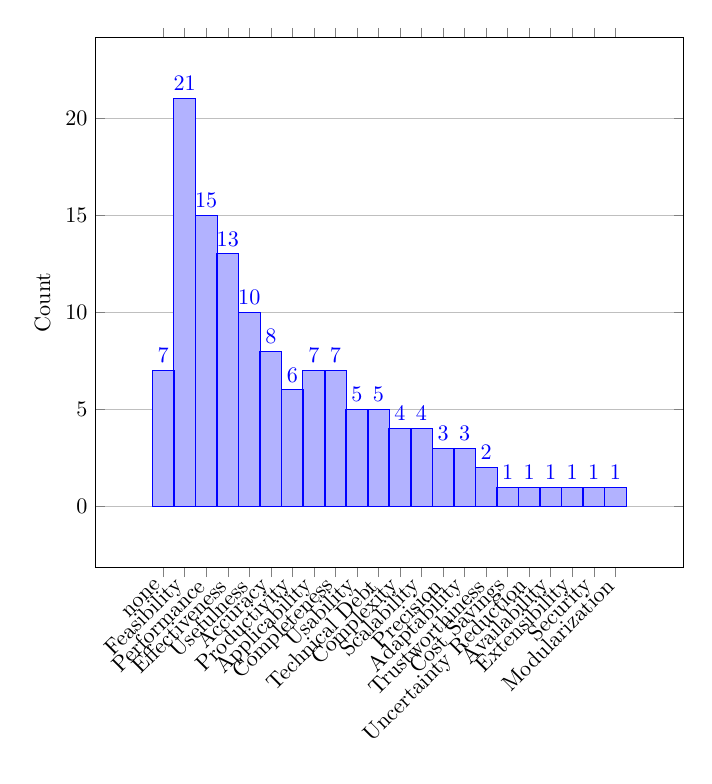
\begin{tikzpicture}[scale=.8]
\begin{axis}[ ybar, ymajorgrids, enlargelimits=0.15, legend style={at={(0.5,-0.15)}, anchor=north,legend columns=-1},
    width=.90\linewidth,height=10cm,
    nodes near coords, %nodes near coords align=below,
    ylabel={Count}, ymin=0,
    x tick label style={rotate=45,anchor=east},
    xtick={1,2,3,4,5,6,7,8,9,10,11,12,13,14,15,16,17,18,19,20,21,22},
    xticklabels={ none, Feasibility, Performance, Effectiveness, Usefulness, Accuracy,  Productivity, Applicability, Completeness, Usability, Technical Debt, Complexity, Scalability, Precision, Adaptability, Trustworthiness, Cost Savings, Uncertainty Reduction, Availability, Extensibility, Security, Modularization
}
    %xlabel={Property Instance}    
    ]
  \addplot coordinates { (1,7)  (2,21)  (3,15)  (4,13)  (5,10)  (6,8)  (7,6)  (8,7)  (9,7)  (10,5)  (11,5)  (12,4)  (13,4)  (14,3)  (15,3)  (16,2)  (17,1)  (18,1)  (19,1)  (20,1)  (21,1)  (22,1)   };
\end{axis}
\end{tikzpicture}
\end{center}
%\caption{Histogramm f\"ur Property Instance (126)}
%\label{fig:histo_propertyinstance}
%\end{figure}


%\subsection{Histogramm f\"ur Evaluation Method (88)}
%\begin{figure}
\begin{center}
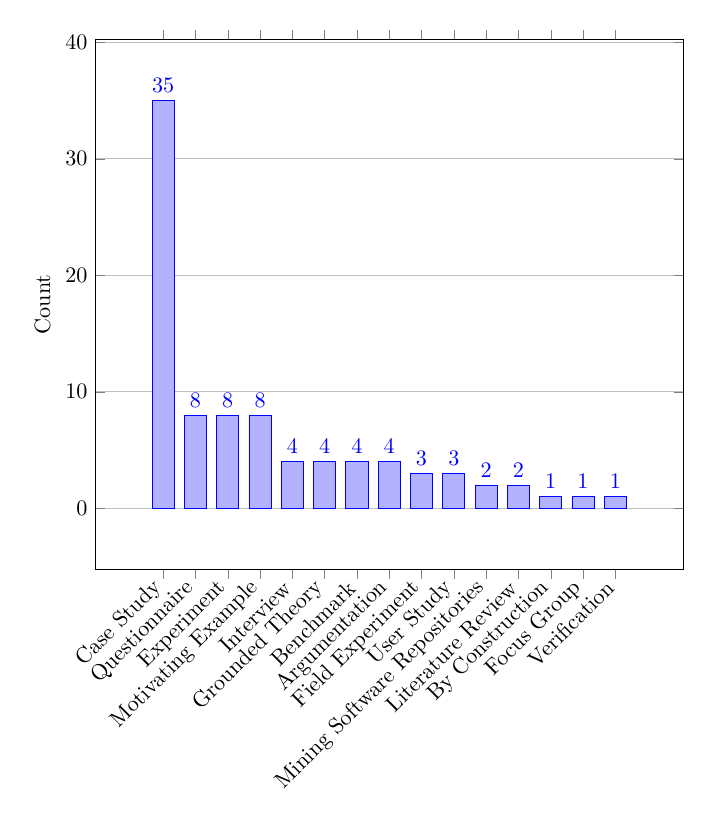
\begin{tikzpicture}[scale=.8]
\begin{axis}[ ybar, ymajorgrids, enlargelimits=0.15, legend style={at={(0.5,-0.15)}, anchor=north,legend columns=-1},
    width=.90\linewidth,height=10cm,
    nodes near coords, %nodes near coords align=below,
    ylabel={Count}, ymin=0,
    x tick label style={rotate=45,anchor=east},
    xtick={1,2,3,4,5,6,7,8,9,10,11,12,13,14,15},
    xticklabels={Case Study, Questionnaire, Experiment, Motivating Example, Interview, Grounded Theory, Benchmark, Argumentation, Field Experiment, User Study, Mining Software Repositories, Literature Review, By Construction,Focus Group,Verification
}
    %xlabel={Evaluation Method}    
    ]
  \addplot coordinates { (1,35)  (2,8)  (3,8)  (4,8)  (5,4)  (6,4)  (7,4)  (8,4)  (9,3)  (10,3)  (11,2)  (12,2)  (13,1)  (14,1)  (15,1)   };
\end{axis}
\end{tikzpicture}
\end{center}
%\caption{Histogramm f\"ur Evaluation Method (88)}
%\label{fig:histo_evaluationmethod}
%\end{figure}


%\subsection{Portfolio f\"ur Property Instance und Evaluation Method (Gr\"o\ss{}e entspricht der Anzahl)}
%\begin{figure}
\begin{center}
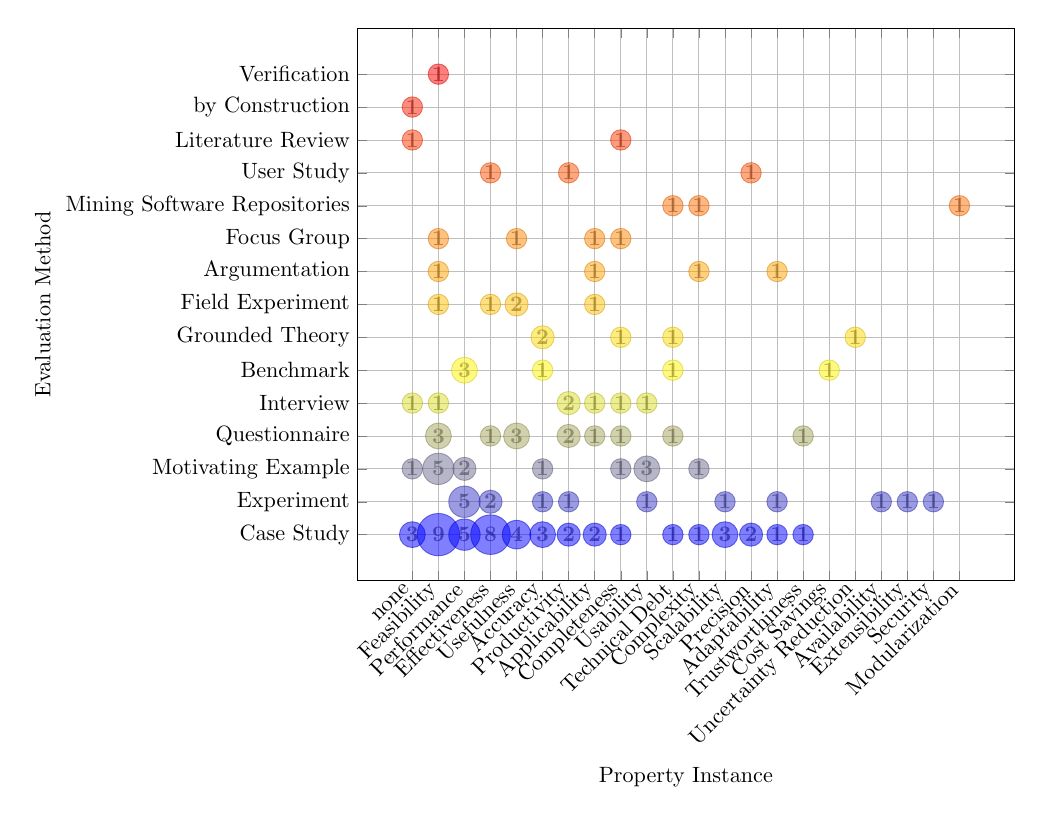
\begin{tikzpicture}[scale=.8]
\begin{axis}[scatter,
    width=.99\linewidth,
    cycle multi list=Spectral,
    every axis plot/.append style={draw, fill, fill opacity=0.5},
    scatter src=y,
    nodes near coords style={color=black,font=\small},
    %enlargelimits=0.15,
    x tick label style={rotate=45,anchor=east},
    xtick={0,1,2,3,4,5,6,7,8,9,10,11,12,13,14,15,16,17,18,19,20,21}, xticklabels={none,Feasibility,Performance,Effectiveness,Usefulness,Accuracy,Productivity,Applicability,Completeness,Usability,Technical Debt,Complexity,Scalability,Precision,Adaptability,Trustworthiness,Cost Savings,Uncertainty Reduction,Availability,Extensibility,Security,Modularization},
    xlabel={Property Instance},
    ytick={0,1,2,3,4,5,6,7,8,9,10,11,12,13,14}, yticklabels={Case Study,Experiment,Motivating Example,Questionnaire,Interview,Benchmark,Grounded Theory,Field Experiment,Argumentation,Focus Group,Mining Software Repositories,User Study,Literature Review,by Construction,Verification},
    ylabel={Evaluation Method},
    grid=both
]

\addplot[mark size=5.860,opacity=0.5,text=black] coordinates { (0,0) } node[text=black,font=\bfseries] {3};
\addplot[mark size=4.620,opacity=0.5,text=black] coordinates { (0,2) } node[text=black,font=\bfseries] {1};
\addplot[mark size=4.620,opacity=0.5,text=black] coordinates { (0,4) } node[text=black,font=\bfseries] {1};
\addplot[mark size=4.620,opacity=0.5,text=black] coordinates { (0,12) } node[text=black,font=\bfseries] {1};
\addplot[mark size=4.620,opacity=0.5,text=black] coordinates { (0,13) } node[text=black,font=\bfseries] {1};
\addplot[mark size=9.581,opacity=0.5,text=black] coordinates { (1,0) } node[text=black,font=\bfseries] {9};
\addplot[mark size=7.101,opacity=0.5,text=black] coordinates { (1,2) } node[text=black,font=\bfseries] {5};
\addplot[mark size=5.860,opacity=0.5,text=black] coordinates { (1,3) } node[text=black,font=\bfseries] {3};
\addplot[mark size=4.620,opacity=0.5,text=black] coordinates { (1,4) } node[text=black,font=\bfseries] {1};
\addplot[mark size=4.620,opacity=0.5,text=black] coordinates { (1,7) } node[text=black,font=\bfseries] {1};
\addplot[mark size=4.620,opacity=0.5,text=black] coordinates { (1,8) } node[text=black,font=\bfseries] {1};
\addplot[mark size=4.620,opacity=0.5,text=black] coordinates { (1,9) } node[text=black,font=\bfseries] {1};
\addplot[mark size=4.620,opacity=0.5,text=black] coordinates { (1,14) } node[text=black,font=\bfseries] {1};
\addplot[mark size=7.101,opacity=0.5,text=black] coordinates { (2,0) } node[text=black,font=\bfseries] {5};
\addplot[mark size=7.101,opacity=0.5,text=black] coordinates { (2,1) } node[text=black,font=\bfseries] {5};
\addplot[mark size=5.240,opacity=0.5,text=black] coordinates { (2,2) } node[text=black,font=\bfseries] {2};
\addplot[mark size=5.860,opacity=0.5,text=black] coordinates { (2,5) } node[text=black,font=\bfseries] {3};
\addplot[mark size=8.961,opacity=0.5,text=black] coordinates { (3,0) } node[text=black,font=\bfseries] {8};
\addplot[mark size=5.240,opacity=0.5,text=black] coordinates { (3,1) } node[text=black,font=\bfseries] {2};
\addplot[mark size=4.620,opacity=0.5,text=black] coordinates { (3,3) } node[text=black,font=\bfseries] {1};
\addplot[mark size=4.620,opacity=0.5,text=black] coordinates { (3,7) } node[text=black,font=\bfseries] {1};
\addplot[mark size=4.620,opacity=0.5,text=black] coordinates { (3,11) } node[text=black,font=\bfseries] {1};
\addplot[mark size=6.481,opacity=0.5,text=black] coordinates { (4,0) } node[text=black,font=\bfseries] {4};
\addplot[mark size=5.860,opacity=0.5,text=black] coordinates { (4,3) } node[text=black,font=\bfseries] {3};
\addplot[mark size=5.240,opacity=0.5,text=black] coordinates { (4,7) } node[text=black,font=\bfseries] {2};
\addplot[mark size=4.620,opacity=0.5,text=black] coordinates { (4,9) } node[text=black,font=\bfseries] {1};
\addplot[mark size=5.860,opacity=0.5,text=black] coordinates { (5,0) } node[text=black,font=\bfseries] {3};
\addplot[mark size=4.620,opacity=0.5,text=black] coordinates { (5,1) } node[text=black,font=\bfseries] {1};
\addplot[mark size=4.620,opacity=0.5,text=black] coordinates { (5,2) } node[text=black,font=\bfseries] {1};
\addplot[mark size=4.620,opacity=0.5,text=black] coordinates { (5,5) } node[text=black,font=\bfseries] {1};
\addplot[mark size=5.240,opacity=0.5,text=black] coordinates { (5,6) } node[text=black,font=\bfseries] {2};
\addplot[mark size=5.240,opacity=0.5,text=black] coordinates { (6,0) } node[text=black,font=\bfseries] {2};
\addplot[mark size=4.620,opacity=0.5,text=black] coordinates { (6,1) } node[text=black,font=\bfseries] {1};
\addplot[mark size=5.240,opacity=0.5,text=black] coordinates { (6,3) } node[text=black,font=\bfseries] {2};
\addplot[mark size=5.240,opacity=0.5,text=black] coordinates { (6,4) } node[text=black,font=\bfseries] {2};
\addplot[mark size=4.620,opacity=0.5,text=black] coordinates { (6,11) } node[text=black,font=\bfseries] {1};
\addplot[mark size=5.240,opacity=0.5,text=black] coordinates { (7,0) } node[text=black,font=\bfseries] {2};
\addplot[mark size=4.620,opacity=0.5,text=black] coordinates { (7,3) } node[text=black,font=\bfseries] {1};
\addplot[mark size=4.620,opacity=0.5,text=black] coordinates { (7,4) } node[text=black,font=\bfseries] {1};
\addplot[mark size=4.620,opacity=0.5,text=black] coordinates { (7,7) } node[text=black,font=\bfseries] {1};
\addplot[mark size=4.620,opacity=0.5,text=black] coordinates { (7,8) } node[text=black,font=\bfseries] {1};
\addplot[mark size=4.620,opacity=0.5,text=black] coordinates { (7,9) } node[text=black,font=\bfseries] {1};
\addplot[mark size=4.620,opacity=0.5,text=black] coordinates { (8,0) } node[text=black,font=\bfseries] {1};
\addplot[mark size=4.620,opacity=0.5,text=black] coordinates { (8,2) } node[text=black,font=\bfseries] {1};
\addplot[mark size=4.620,opacity=0.5,text=black] coordinates { (8,3) } node[text=black,font=\bfseries] {1};
\addplot[mark size=4.620,opacity=0.5,text=black] coordinates { (8,4) } node[text=black,font=\bfseries] {1};
\addplot[mark size=4.620,opacity=0.5,text=black] coordinates { (8,6) } node[text=black,font=\bfseries] {1};
\addplot[mark size=4.620,opacity=0.5,text=black] coordinates { (8,9) } node[text=black,font=\bfseries] {1};
\addplot[mark size=4.620,opacity=0.5,text=black] coordinates { (8,12) } node[text=black,font=\bfseries] {1};
\addplot[mark size=4.620,opacity=0.5,text=black] coordinates { (9,1) } node[text=black,font=\bfseries] {1};
\addplot[mark size=5.860,opacity=0.5,text=black] coordinates { (9,2) } node[text=black,font=\bfseries] {3};
\addplot[mark size=4.620,opacity=0.5,text=black] coordinates { (9,4) } node[text=black,font=\bfseries] {1};
\addplot[mark size=4.620,opacity=0.5,text=black] coordinates { (10,0) } node[text=black,font=\bfseries] {1};
\addplot[mark size=4.620,opacity=0.5,text=black] coordinates { (10,3) } node[text=black,font=\bfseries] {1};
\addplot[mark size=4.620,opacity=0.5,text=black] coordinates { (10,5) } node[text=black,font=\bfseries] {1};
\addplot[mark size=4.620,opacity=0.5,text=black] coordinates { (10,6) } node[text=black,font=\bfseries] {1};
\addplot[mark size=4.620,opacity=0.5,text=black] coordinates { (10,10) } node[text=black,font=\bfseries] {1};
\addplot[mark size=4.620,opacity=0.5,text=black] coordinates { (11,0) } node[text=black,font=\bfseries] {1};
\addplot[mark size=4.620,opacity=0.5,text=black] coordinates { (11,2) } node[text=black,font=\bfseries] {1};
\addplot[mark size=4.620,opacity=0.5,text=black] coordinates { (11,8) } node[text=black,font=\bfseries] {1};
\addplot[mark size=4.620,opacity=0.5,text=black] coordinates { (11,10) } node[text=black,font=\bfseries] {1};
\addplot[mark size=5.860,opacity=0.5,text=black] coordinates { (12,0) } node[text=black,font=\bfseries] {3};
\addplot[mark size=4.620,opacity=0.5,text=black] coordinates { (12,1) } node[text=black,font=\bfseries] {1};
\addplot[mark size=5.240,opacity=0.5,text=black] coordinates { (13,0) } node[text=black,font=\bfseries] {2};
\addplot[mark size=4.620,opacity=0.5,text=black] coordinates { (13,11) } node[text=black,font=\bfseries] {1};
\addplot[mark size=4.620,opacity=0.5,text=black] coordinates { (14,0) } node[text=black,font=\bfseries] {1};
\addplot[mark size=4.620,opacity=0.5,text=black] coordinates { (14,1) } node[text=black,font=\bfseries] {1};
\addplot[mark size=4.620,opacity=0.5,text=black] coordinates { (14,8) } node[text=black,font=\bfseries] {1};
\addplot[mark size=4.620,opacity=0.5,text=black] coordinates { (15,0) } node[text=black,font=\bfseries] {1};
\addplot[mark size=4.620,opacity=0.5,text=black] coordinates { (15,3) } node[text=black,font=\bfseries] {1};
\addplot[mark size=4.620,opacity=0.5,text=black] coordinates { (16,5) } node[text=black,font=\bfseries] {1};
\addplot[mark size=4.620,opacity=0.5,text=black] coordinates { (17,6) } node[text=black,font=\bfseries] {1};
\addplot[mark size=4.620,opacity=0.5,text=black] coordinates { (18,1) } node[text=black,font=\bfseries] {1};
\addplot[mark size=4.620,opacity=0.5,text=black] coordinates { (19,1) } node[text=black,font=\bfseries] {1};
\addplot[mark size=4.620,opacity=0.5,text=black] coordinates { (20,1) } node[text=black,font=\bfseries] {1};
\addplot[mark size=4.620,opacity=0.5,text=black] coordinates { (21,10) } node[text=black,font=\bfseries] {1};


\end{axis}
\end{tikzpicture}
\end{center}
%\caption{Portfolio f\"ur Property Instance und Evaluation Method (Gr\"o\ss{}e entspricht der Anzahl)}\label{fig:port_propertyinstance_evaluationmethod}
%\end{figure}


%\subsection{Portfolio f\"ur Evaluation Method und Property Instance (Gr\"o\ss{}e entspricht der Anzahl)}
%\begin{figure}
\begin{center}
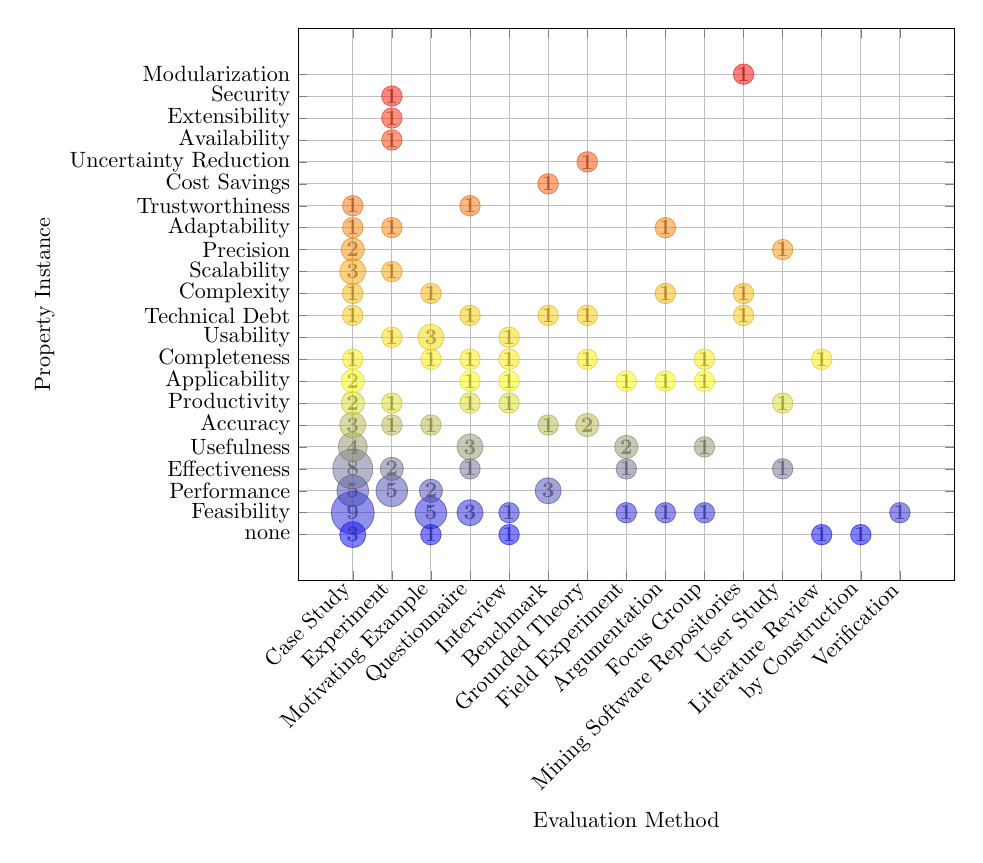
\begin{tikzpicture}[scale=.8]
\begin{axis}[scatter,
    width=.99\linewidth,
    cycle multi list=Spectral,
    every axis plot/.append style={draw, fill, fill opacity=0.5},
    scatter src=y,
    nodes near coords style={color=black,font=\small},
    %enlargelimits=0.15,
    x tick label style={rotate=45,anchor=east},
    xtick={0,1,2,3,4,5,6,7,8,9,10,11,12,13,14}, xticklabels={Case Study,Experiment,Motivating Example,Questionnaire,Interview,Benchmark,Grounded Theory,Field Experiment,Argumentation,Focus Group,Mining Software Repositories,User Study,Literature Review,by Construction,Verification},
    xlabel={Evaluation Method},
    ytick={0,1,2,3,4,5,6,7,8,9,10,11,12,13,14,15,16,17,18,19,20,21}, yticklabels={none,Feasibility,Performance,Effectiveness,Usefulness,Accuracy,Productivity,Applicability,Completeness,Usability,Technical Debt,Complexity,Scalability,Precision,Adaptability,Trustworthiness,Cost Savings,Uncertainty Reduction,Availability,Extensibility,Security,Modularization},
    ylabel={Property Instance},
    grid=both
]

\addplot[mark size=5.890,opacity=0.5,text=black] coordinates { (0,0) } node[text=black,font=\bfseries] {3};
\addplot[mark size=9.669,opacity=0.5,text=black] coordinates { (0,1) } node[text=black,font=\bfseries] {9};
\addplot[mark size=7.150,opacity=0.5,text=black] coordinates { (0,2) } node[text=black,font=\bfseries] {5};
\addplot[mark size=9.039,opacity=0.5,text=black] coordinates { (0,3) } node[text=black,font=\bfseries] {8};
\addplot[mark size=6.520,opacity=0.5,text=black] coordinates { (0,4) } node[text=black,font=\bfseries] {4};
\addplot[mark size=5.890,opacity=0.5,text=black] coordinates { (0,5) } node[text=black,font=\bfseries] {3};
\addplot[mark size=5.260,opacity=0.5,text=black] coordinates { (0,6) } node[text=black,font=\bfseries] {2};
\addplot[mark size=5.260,opacity=0.5,text=black] coordinates { (0,7) } node[text=black,font=\bfseries] {2};
\addplot[mark size=4.630,opacity=0.5,text=black] coordinates { (0,8) } node[text=black,font=\bfseries] {1};
\addplot[mark size=4.630,opacity=0.5,text=black] coordinates { (0,10) } node[text=black,font=\bfseries] {1};
\addplot[mark size=4.630,opacity=0.5,text=black] coordinates { (0,11) } node[text=black,font=\bfseries] {1};
\addplot[mark size=5.890,opacity=0.5,text=black] coordinates { (0,12) } node[text=black,font=\bfseries] {3};
\addplot[mark size=5.260,opacity=0.5,text=black] coordinates { (0,13) } node[text=black,font=\bfseries] {2};
\addplot[mark size=4.630,opacity=0.5,text=black] coordinates { (0,14) } node[text=black,font=\bfseries] {1};
\addplot[mark size=4.630,opacity=0.5,text=black] coordinates { (0,15) } node[text=black,font=\bfseries] {1};
\addplot[mark size=7.150,opacity=0.5,text=black] coordinates { (1,2) } node[text=black,font=\bfseries] {5};
\addplot[mark size=5.260,opacity=0.5,text=black] coordinates { (1,3) } node[text=black,font=\bfseries] {2};
\addplot[mark size=4.630,opacity=0.5,text=black] coordinates { (1,5) } node[text=black,font=\bfseries] {1};
\addplot[mark size=4.630,opacity=0.5,text=black] coordinates { (1,6) } node[text=black,font=\bfseries] {1};
\addplot[mark size=4.630,opacity=0.5,text=black] coordinates { (1,9) } node[text=black,font=\bfseries] {1};
\addplot[mark size=4.630,opacity=0.5,text=black] coordinates { (1,12) } node[text=black,font=\bfseries] {1};
\addplot[mark size=4.630,opacity=0.5,text=black] coordinates { (1,14) } node[text=black,font=\bfseries] {1};
\addplot[mark size=4.630,opacity=0.5,text=black] coordinates { (1,18) } node[text=black,font=\bfseries] {1};
\addplot[mark size=4.630,opacity=0.5,text=black] coordinates { (1,19) } node[text=black,font=\bfseries] {1};
\addplot[mark size=4.630,opacity=0.5,text=black] coordinates { (1,20) } node[text=black,font=\bfseries] {1};
\addplot[mark size=4.630,opacity=0.5,text=black] coordinates { (2,0) } node[text=black,font=\bfseries] {1};
\addplot[mark size=7.150,opacity=0.5,text=black] coordinates { (2,1) } node[text=black,font=\bfseries] {5};
\addplot[mark size=5.260,opacity=0.5,text=black] coordinates { (2,2) } node[text=black,font=\bfseries] {2};
\addplot[mark size=4.630,opacity=0.5,text=black] coordinates { (2,5) } node[text=black,font=\bfseries] {1};
\addplot[mark size=4.630,opacity=0.5,text=black] coordinates { (2,8) } node[text=black,font=\bfseries] {1};
\addplot[mark size=5.890,opacity=0.5,text=black] coordinates { (2,9) } node[text=black,font=\bfseries] {3};
\addplot[mark size=4.630,opacity=0.5,text=black] coordinates { (2,11) } node[text=black,font=\bfseries] {1};
\addplot[mark size=5.890,opacity=0.5,text=black] coordinates { (3,1) } node[text=black,font=\bfseries] {3};
\addplot[mark size=4.630,opacity=0.5,text=black] coordinates { (3,3) } node[text=black,font=\bfseries] {1};
\addplot[mark size=5.890,opacity=0.5,text=black] coordinates { (3,4) } node[text=black,font=\bfseries] {3};
\addplot[mark size=4.630,opacity=0.5,text=black] coordinates { (3,6) } node[text=black,font=\bfseries] {1};
\addplot[mark size=4.630,opacity=0.5,text=black] coordinates { (3,7) } node[text=black,font=\bfseries] {1};
\addplot[mark size=4.630,opacity=0.5,text=black] coordinates { (3,8) } node[text=black,font=\bfseries] {1};
\addplot[mark size=4.630,opacity=0.5,text=black] coordinates { (3,10) } node[text=black,font=\bfseries] {1};
\addplot[mark size=4.630,opacity=0.5,text=black] coordinates { (3,15) } node[text=black,font=\bfseries] {1};
\addplot[mark size=4.630,opacity=0.5,text=black] coordinates { (4,0) } node[text=black,font=\bfseries] {1};
\addplot[mark size=4.630,opacity=0.5,text=black] coordinates { (4,1) } node[text=black,font=\bfseries] {1};
\addplot[mark size=4.630,opacity=0.5,text=black] coordinates { (4,6) } node[text=black,font=\bfseries] {1};
\addplot[mark size=4.630,opacity=0.5,text=black] coordinates { (4,7) } node[text=black,font=\bfseries] {1};
\addplot[mark size=4.630,opacity=0.5,text=black] coordinates { (4,8) } node[text=black,font=\bfseries] {1};
\addplot[mark size=4.630,opacity=0.5,text=black] coordinates { (4,9) } node[text=black,font=\bfseries] {1};
\addplot[mark size=5.890,opacity=0.5,text=black] coordinates { (5,2) } node[text=black,font=\bfseries] {3};
\addplot[mark size=4.630,opacity=0.5,text=black] coordinates { (5,5) } node[text=black,font=\bfseries] {1};
\addplot[mark size=4.630,opacity=0.5,text=black] coordinates { (5,10) } node[text=black,font=\bfseries] {1};
\addplot[mark size=4.630,opacity=0.5,text=black] coordinates { (5,16) } node[text=black,font=\bfseries] {1};
\addplot[mark size=5.260,opacity=0.5,text=black] coordinates { (6,5) } node[text=black,font=\bfseries] {2};
\addplot[mark size=4.630,opacity=0.5,text=black] coordinates { (6,8) } node[text=black,font=\bfseries] {1};
\addplot[mark size=4.630,opacity=0.5,text=black] coordinates { (6,10) } node[text=black,font=\bfseries] {1};
\addplot[mark size=4.630,opacity=0.5,text=black] coordinates { (6,17) } node[text=black,font=\bfseries] {1};
\addplot[mark size=4.630,opacity=0.5,text=black] coordinates { (7,1) } node[text=black,font=\bfseries] {1};
\addplot[mark size=4.630,opacity=0.5,text=black] coordinates { (7,3) } node[text=black,font=\bfseries] {1};
\addplot[mark size=5.260,opacity=0.5,text=black] coordinates { (7,4) } node[text=black,font=\bfseries] {2};
\addplot[mark size=4.630,opacity=0.5,text=black] coordinates { (7,7) } node[text=black,font=\bfseries] {1};
\addplot[mark size=4.630,opacity=0.5,text=black] coordinates { (8,1) } node[text=black,font=\bfseries] {1};
\addplot[mark size=4.630,opacity=0.5,text=black] coordinates { (8,7) } node[text=black,font=\bfseries] {1};
\addplot[mark size=4.630,opacity=0.5,text=black] coordinates { (8,11) } node[text=black,font=\bfseries] {1};
\addplot[mark size=4.630,opacity=0.5,text=black] coordinates { (8,14) } node[text=black,font=\bfseries] {1};
\addplot[mark size=4.630,opacity=0.5,text=black] coordinates { (9,1) } node[text=black,font=\bfseries] {1};
\addplot[mark size=4.630,opacity=0.5,text=black] coordinates { (9,4) } node[text=black,font=\bfseries] {1};
\addplot[mark size=4.630,opacity=0.5,text=black] coordinates { (9,7) } node[text=black,font=\bfseries] {1};
\addplot[mark size=4.630,opacity=0.5,text=black] coordinates { (9,8) } node[text=black,font=\bfseries] {1};
\addplot[mark size=4.630,opacity=0.5,text=black] coordinates { (10,10) } node[text=black,font=\bfseries] {1};
\addplot[mark size=4.630,opacity=0.5,text=black] coordinates { (10,11) } node[text=black,font=\bfseries] {1};
\addplot[mark size=4.630,opacity=0.5,text=black] coordinates { (10,21) } node[text=black,font=\bfseries] {1};
\addplot[mark size=4.630,opacity=0.5,text=black] coordinates { (11,3) } node[text=black,font=\bfseries] {1};
\addplot[mark size=4.630,opacity=0.5,text=black] coordinates { (11,6) } node[text=black,font=\bfseries] {1};
\addplot[mark size=4.630,opacity=0.5,text=black] coordinates { (11,13) } node[text=black,font=\bfseries] {1};
\addplot[mark size=4.630,opacity=0.5,text=black] coordinates { (12,0) } node[text=black,font=\bfseries] {1};
\addplot[mark size=4.630,opacity=0.5,text=black] coordinates { (12,8) } node[text=black,font=\bfseries] {1};
\addplot[mark size=4.630,opacity=0.5,text=black] coordinates { (13,0) } node[text=black,font=\bfseries] {1};
\addplot[mark size=4.630,opacity=0.5,text=black] coordinates { (14,1) } node[text=black,font=\bfseries] {1};


\end{axis}
\end{tikzpicture}
\end{center}
%\caption{Portfolio f\"ur Evaluation Method und Property Instance (Gr\"o\ss{}e entspricht der Anzahl)}\label{fig:port_evaluationmethod_propertyinstance}
%\end{figure}



\section{Evaluation Method vs Threats to Validity}

%\subsection{Histogramm f\"ur Evaluation Method (88)}
%\begin{figure}
\begin{center}
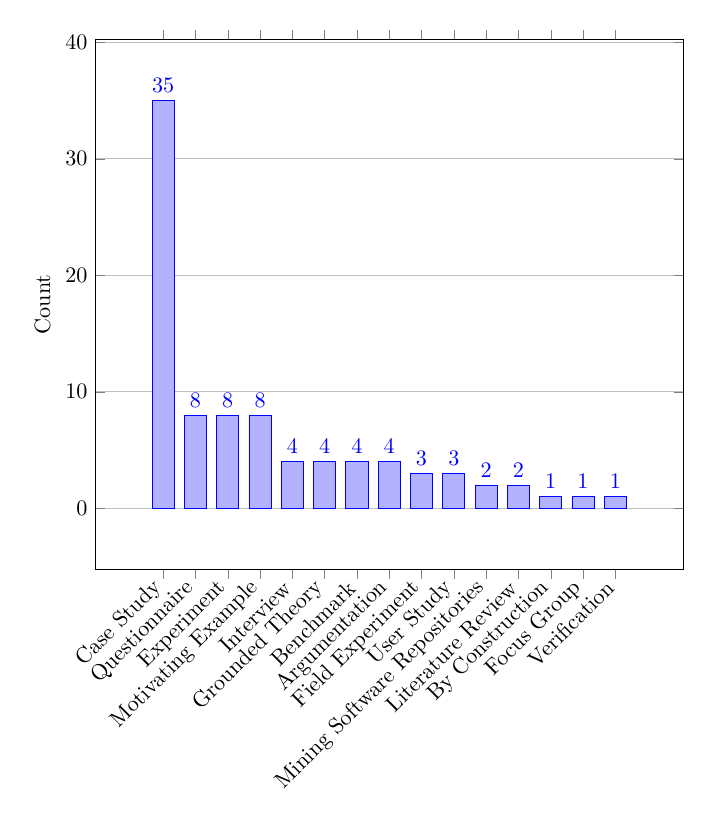
\begin{tikzpicture}[scale=.8]
\begin{axis}[ ybar, ymajorgrids, enlargelimits=0.15, legend style={at={(0.5,-0.15)}, anchor=north,legend columns=-1},
    width=.90\linewidth,height=10cm,
    nodes near coords, %nodes near coords align=below,
    ylabel={Count}, ymin=0,
    x tick label style={rotate=45,anchor=east},
    xtick={1,2,3,4,5,6,7,8,9,10,11,12,13,14,15},
    xticklabels={Case Study, Questionnaire, Experiment, Motivating Example, Interview, Grounded Theory, Benchmark, Argumentation, Field Experiment, User Study, Mining Software Repositories, Literature Review, By Construction,Focus Group,Verification
}
    %xlabel={Evaluation Method}    
    ]
  \addplot coordinates { (1,35)  (2,8)  (3,8)  (4,8)  (5,4)  (6,4)  (7,4)  (8,4)  (9,3)  (10,3)  (11,2)  (12,2)  (13,1)  (14,1)  (15,1)   };
\end{axis}
\end{tikzpicture}
\end{center}
%\caption{Histogramm f\"ur Evaluation Method (88)}
%\label{fig:histo_evaluationmethod}
%\end{figure}


%\subsection{Histogramm f\"ur Threats to Validity (167)}
%\begin{figure}
\begin{center}
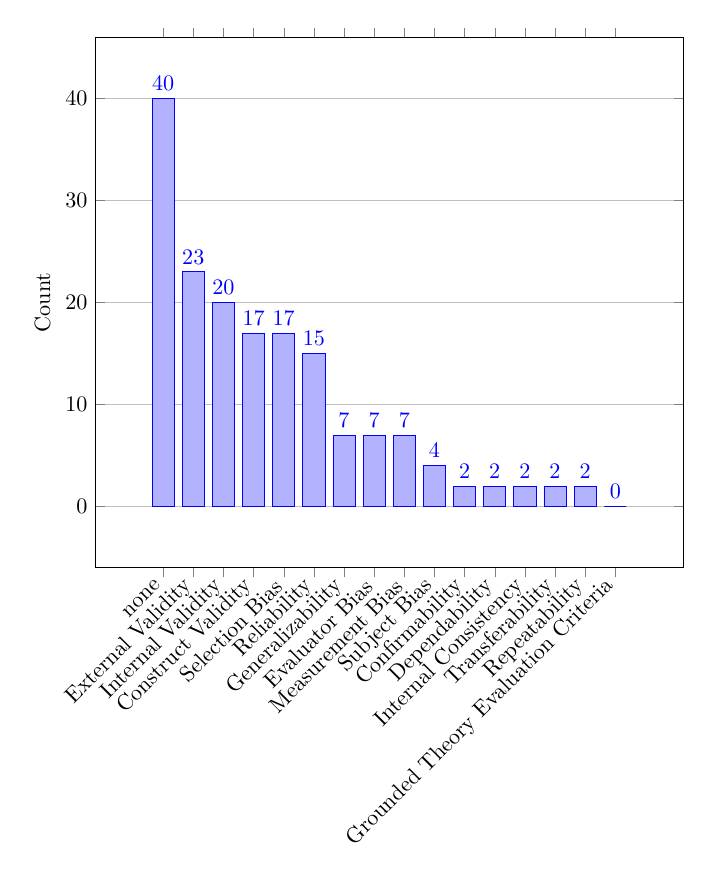
\begin{tikzpicture}[scale=.8]
\begin{axis}[ ybar, ymajorgrids, enlargelimits=0.15, legend style={at={(0.5,-0.15)}, anchor=north,legend columns=-1},
    width=.90\linewidth,height=10cm,
    nodes near coords, %nodes near coords align=below,
    ylabel={Count}, ymin=0,
    x tick label style={rotate=45,anchor=east},
    xtick={1,2,3,4,5,6,7,8,9,10,11,12,13,14,15,16},
    xticklabels={none, External Validity, Internal Validity, Construct Validity, Selection Bias, Reliability, Generalizability, Evaluator Bias, Measurement Bias, Subject Bias, Confirmability, Dependability, Internal Consistency ,Transferability, Repeatability, Grounded Theory Evaluation Criteria
}
    %xlabel={Threats to Validity}    
    ]
  \addplot coordinates { (1,40)  (2,23)  (3,20)  (4,17)  (5,17)  (6,15)  (7,7)  (8,7)  (9,7)  (10,4)  (11,2)  (12,2)  (13,2)  (14,2)  (15,2)  (16,0)   };
\end{axis}
\end{tikzpicture}
\end{center}
%\caption{Histogramm f\"ur Threats to Validity (167)}
%\label{fig:histo_threatstovalidity}
%\end{figure}


%\subsection{Portfolio f\"ur Evaluation Method und Threats to Validity (Gr\"o\ss{}e entspricht der Anzahl)}
%\begin{figure}
\begin{center}
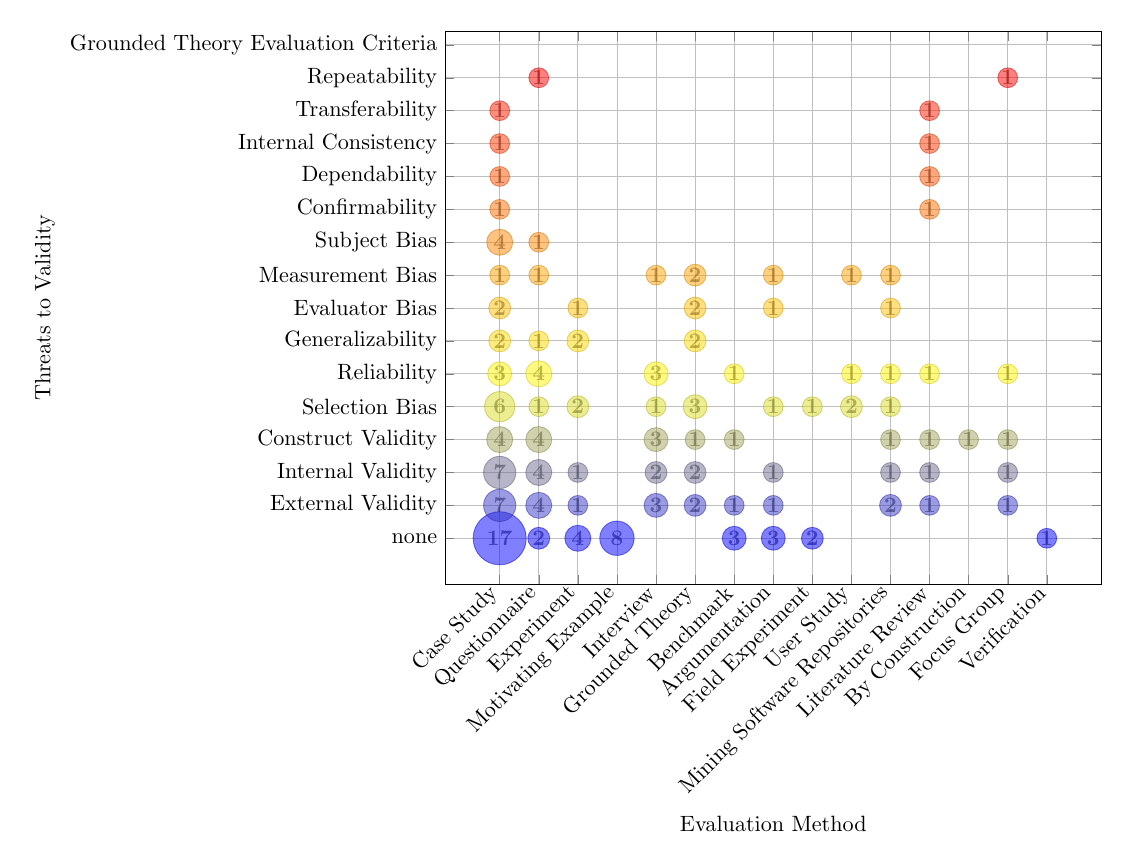
\begin{tikzpicture}[scale=.8]
\begin{axis}[scatter,
    width=.99\linewidth,
    cycle multi list=Spectral,
    every axis plot/.append style={draw, fill, fill opacity=0.5},
    scatter src=y,
    nodes near coords style={color=black,font=\small},
    %enlargelimits=0.15,
    x tick label style={rotate=45,anchor=east},
    xtick={0,1,2,3,4,5,6,7,8,9,10,11,12,13,14}, xticklabels={Case Study,Questionnaire,Experiment,Motivating Example,Interview,Grounded Theory,Benchmark,Argumentation,Field Experiment,User Study,Mining Software Repositories,Literature Review,By Construction,Focus Group,Verification},
    xlabel={Evaluation Method},
    ytick={0,1,2,3,4,5,6,7,8,9,10,11,12,13,14,15}, yticklabels={none,External Validity,Internal Validity,Construct Validity,Selection Bias,Reliability,Generalizability,Evaluator Bias,Measurement Bias,Subject Bias,Confirmability,Dependability,Internal Consistency,Transferability,Repeatability,Grounded Theory Evaluation Criteria},
    ylabel={Threats to Validity},
    grid=both
]

\addplot[mark size=12.000,opacity=0.5,text=black] coordinates { (0,0) } node[text=black,font=\bfseries] {17};
\addplot[mark size=7.294,opacity=0.5,text=black] coordinates { (0,1) } node[text=black,font=\bfseries] {7};
\addplot[mark size=7.294,opacity=0.5,text=black] coordinates { (0,2) } node[text=black,font=\bfseries] {7};
\addplot[mark size=5.882,opacity=0.5,text=black] coordinates { (0,3) } node[text=black,font=\bfseries] {4};
\addplot[mark size=6.824,opacity=0.5,text=black] coordinates { (0,4) } node[text=black,font=\bfseries] {6};
\addplot[mark size=5.412,opacity=0.5,text=black] coordinates { (0,5) } node[text=black,font=\bfseries] {3};
\addplot[mark size=4.941,opacity=0.5,text=black] coordinates { (0,6) } node[text=black,font=\bfseries] {2};
\addplot[mark size=4.941,opacity=0.5,text=black] coordinates { (0,7) } node[text=black,font=\bfseries] {2};
\addplot[mark size=4.471,opacity=0.5,text=black] coordinates { (0,8) } node[text=black,font=\bfseries] {1};
\addplot[mark size=5.882,opacity=0.5,text=black] coordinates { (0,9) } node[text=black,font=\bfseries] {4};
\addplot[mark size=4.471,opacity=0.5,text=black] coordinates { (0,10) } node[text=black,font=\bfseries] {1};
\addplot[mark size=4.471,opacity=0.5,text=black] coordinates { (0,11) } node[text=black,font=\bfseries] {1};
\addplot[mark size=4.471,opacity=0.5,text=black] coordinates { (0,12) } node[text=black,font=\bfseries] {1};
\addplot[mark size=4.471,opacity=0.5,text=black] coordinates { (0,13) } node[text=black,font=\bfseries] {1};
\addplot[mark size=4.941,opacity=0.5,text=black] coordinates { (1,0) } node[text=black,font=\bfseries] {2};
\addplot[mark size=5.882,opacity=0.5,text=black] coordinates { (1,1) } node[text=black,font=\bfseries] {4};
\addplot[mark size=5.882,opacity=0.5,text=black] coordinates { (1,2) } node[text=black,font=\bfseries] {4};
\addplot[mark size=5.882,opacity=0.5,text=black] coordinates { (1,3) } node[text=black,font=\bfseries] {4};
\addplot[mark size=4.471,opacity=0.5,text=black] coordinates { (1,4) } node[text=black,font=\bfseries] {1};
\addplot[mark size=5.882,opacity=0.5,text=black] coordinates { (1,5) } node[text=black,font=\bfseries] {4};
\addplot[mark size=4.471,opacity=0.5,text=black] coordinates { (1,6) } node[text=black,font=\bfseries] {1};
\addplot[mark size=4.471,opacity=0.5,text=black] coordinates { (1,8) } node[text=black,font=\bfseries] {1};
\addplot[mark size=4.471,opacity=0.5,text=black] coordinates { (1,9) } node[text=black,font=\bfseries] {1};
\addplot[mark size=4.471,opacity=0.5,text=black] coordinates { (1,14) } node[text=black,font=\bfseries] {1};
\addplot[mark size=5.882,opacity=0.5,text=black] coordinates { (2,0) } node[text=black,font=\bfseries] {4};
\addplot[mark size=4.471,opacity=0.5,text=black] coordinates { (2,1) } node[text=black,font=\bfseries] {1};
\addplot[mark size=4.471,opacity=0.5,text=black] coordinates { (2,2) } node[text=black,font=\bfseries] {1};
\addplot[mark size=4.941,opacity=0.5,text=black] coordinates { (2,4) } node[text=black,font=\bfseries] {2};
\addplot[mark size=4.941,opacity=0.5,text=black] coordinates { (2,6) } node[text=black,font=\bfseries] {2};
\addplot[mark size=4.471,opacity=0.5,text=black] coordinates { (2,7) } node[text=black,font=\bfseries] {1};
\addplot[mark size=7.765,opacity=0.5,text=black] coordinates { (3,0) } node[text=black,font=\bfseries] {8};
\addplot[mark size=5.412,opacity=0.5,text=black] coordinates { (4,1) } node[text=black,font=\bfseries] {3};
\addplot[mark size=4.941,opacity=0.5,text=black] coordinates { (4,2) } node[text=black,font=\bfseries] {2};
\addplot[mark size=5.412,opacity=0.5,text=black] coordinates { (4,3) } node[text=black,font=\bfseries] {3};
\addplot[mark size=4.471,opacity=0.5,text=black] coordinates { (4,4) } node[text=black,font=\bfseries] {1};
\addplot[mark size=5.412,opacity=0.5,text=black] coordinates { (4,5) } node[text=black,font=\bfseries] {3};
\addplot[mark size=4.471,opacity=0.5,text=black] coordinates { (4,8) } node[text=black,font=\bfseries] {1};
\addplot[mark size=4.941,opacity=0.5,text=black] coordinates { (5,1) } node[text=black,font=\bfseries] {2};
\addplot[mark size=4.941,opacity=0.5,text=black] coordinates { (5,2) } node[text=black,font=\bfseries] {2};
\addplot[mark size=4.471,opacity=0.5,text=black] coordinates { (5,3) } node[text=black,font=\bfseries] {1};
\addplot[mark size=5.412,opacity=0.5,text=black] coordinates { (5,4) } node[text=black,font=\bfseries] {3};
\addplot[mark size=4.941,opacity=0.5,text=black] coordinates { (5,6) } node[text=black,font=\bfseries] {2};
\addplot[mark size=4.941,opacity=0.5,text=black] coordinates { (5,7) } node[text=black,font=\bfseries] {2};
\addplot[mark size=4.941,opacity=0.5,text=black] coordinates { (5,8) } node[text=black,font=\bfseries] {2};
\addplot[mark size=5.412,opacity=0.5,text=black] coordinates { (6,0) } node[text=black,font=\bfseries] {3};
\addplot[mark size=4.471,opacity=0.5,text=black] coordinates { (6,1) } node[text=black,font=\bfseries] {1};
\addplot[mark size=4.471,opacity=0.5,text=black] coordinates { (6,3) } node[text=black,font=\bfseries] {1};
\addplot[mark size=4.471,opacity=0.5,text=black] coordinates { (6,5) } node[text=black,font=\bfseries] {1};
\addplot[mark size=5.412,opacity=0.5,text=black] coordinates { (7,0) } node[text=black,font=\bfseries] {3};
\addplot[mark size=4.471,opacity=0.5,text=black] coordinates { (7,1) } node[text=black,font=\bfseries] {1};
\addplot[mark size=4.471,opacity=0.5,text=black] coordinates { (7,2) } node[text=black,font=\bfseries] {1};
\addplot[mark size=4.471,opacity=0.5,text=black] coordinates { (7,4) } node[text=black,font=\bfseries] {1};
\addplot[mark size=4.471,opacity=0.5,text=black] coordinates { (7,7) } node[text=black,font=\bfseries] {1};
\addplot[mark size=4.471,opacity=0.5,text=black] coordinates { (7,8) } node[text=black,font=\bfseries] {1};
\addplot[mark size=4.941,opacity=0.5,text=black] coordinates { (8,0) } node[text=black,font=\bfseries] {2};
\addplot[mark size=4.471,opacity=0.5,text=black] coordinates { (8,4) } node[text=black,font=\bfseries] {1};
\addplot[mark size=4.941,opacity=0.5,text=black] coordinates { (9,4) } node[text=black,font=\bfseries] {2};
\addplot[mark size=4.471,opacity=0.5,text=black] coordinates { (9,5) } node[text=black,font=\bfseries] {1};
\addplot[mark size=4.471,opacity=0.5,text=black] coordinates { (9,8) } node[text=black,font=\bfseries] {1};
\addplot[mark size=4.941,opacity=0.5,text=black] coordinates { (10,1) } node[text=black,font=\bfseries] {2};
\addplot[mark size=4.471,opacity=0.5,text=black] coordinates { (10,2) } node[text=black,font=\bfseries] {1};
\addplot[mark size=4.471,opacity=0.5,text=black] coordinates { (10,3) } node[text=black,font=\bfseries] {1};
\addplot[mark size=4.471,opacity=0.5,text=black] coordinates { (10,4) } node[text=black,font=\bfseries] {1};
\addplot[mark size=4.471,opacity=0.5,text=black] coordinates { (10,5) } node[text=black,font=\bfseries] {1};
\addplot[mark size=4.471,opacity=0.5,text=black] coordinates { (10,7) } node[text=black,font=\bfseries] {1};
\addplot[mark size=4.471,opacity=0.5,text=black] coordinates { (10,8) } node[text=black,font=\bfseries] {1};
\addplot[mark size=4.471,opacity=0.5,text=black] coordinates { (11,1) } node[text=black,font=\bfseries] {1};
\addplot[mark size=4.471,opacity=0.5,text=black] coordinates { (11,2) } node[text=black,font=\bfseries] {1};
\addplot[mark size=4.471,opacity=0.5,text=black] coordinates { (11,3) } node[text=black,font=\bfseries] {1};
\addplot[mark size=4.471,opacity=0.5,text=black] coordinates { (11,5) } node[text=black,font=\bfseries] {1};
\addplot[mark size=4.471,opacity=0.5,text=black] coordinates { (11,10) } node[text=black,font=\bfseries] {1};
\addplot[mark size=4.471,opacity=0.5,text=black] coordinates { (11,11) } node[text=black,font=\bfseries] {1};
\addplot[mark size=4.471,opacity=0.5,text=black] coordinates { (11,12) } node[text=black,font=\bfseries] {1};
\addplot[mark size=4.471,opacity=0.5,text=black] coordinates { (11,13) } node[text=black,font=\bfseries] {1};
\addplot[mark size=4.471,opacity=0.5,text=black] coordinates { (12,3) } node[text=black,font=\bfseries] {1};
\addplot[mark size=4.471,opacity=0.5,text=black] coordinates { (13,1) } node[text=black,font=\bfseries] {1};
\addplot[mark size=4.471,opacity=0.5,text=black] coordinates { (13,2) } node[text=black,font=\bfseries] {1};
\addplot[mark size=4.471,opacity=0.5,text=black] coordinates { (13,3) } node[text=black,font=\bfseries] {1};
\addplot[mark size=4.471,opacity=0.5,text=black] coordinates { (13,5) } node[text=black,font=\bfseries] {1};
\addplot[mark size=4.471,opacity=0.5,text=black] coordinates { (13,14) } node[text=black,font=\bfseries] {1};
\addplot[mark size=4.471,opacity=0.5,text=black] coordinates { (14,0) } node[text=black,font=\bfseries] {1};


\end{axis}
\end{tikzpicture}
\end{center}
%\caption{Portfolio f\"ur Evaluation Method und Threats to Validity (Gr\"o\ss{}e entspricht der Anzahl)}\label{fig:port_evaluationmethod_threatstovalidity}
%\end{figure}


%\subsection{Portfolio f\"ur Threats to Validity und Evaluation Method (Gr\"o\ss{}e entspricht der Anzahl)}
%\begin{figure}
\begin{center}
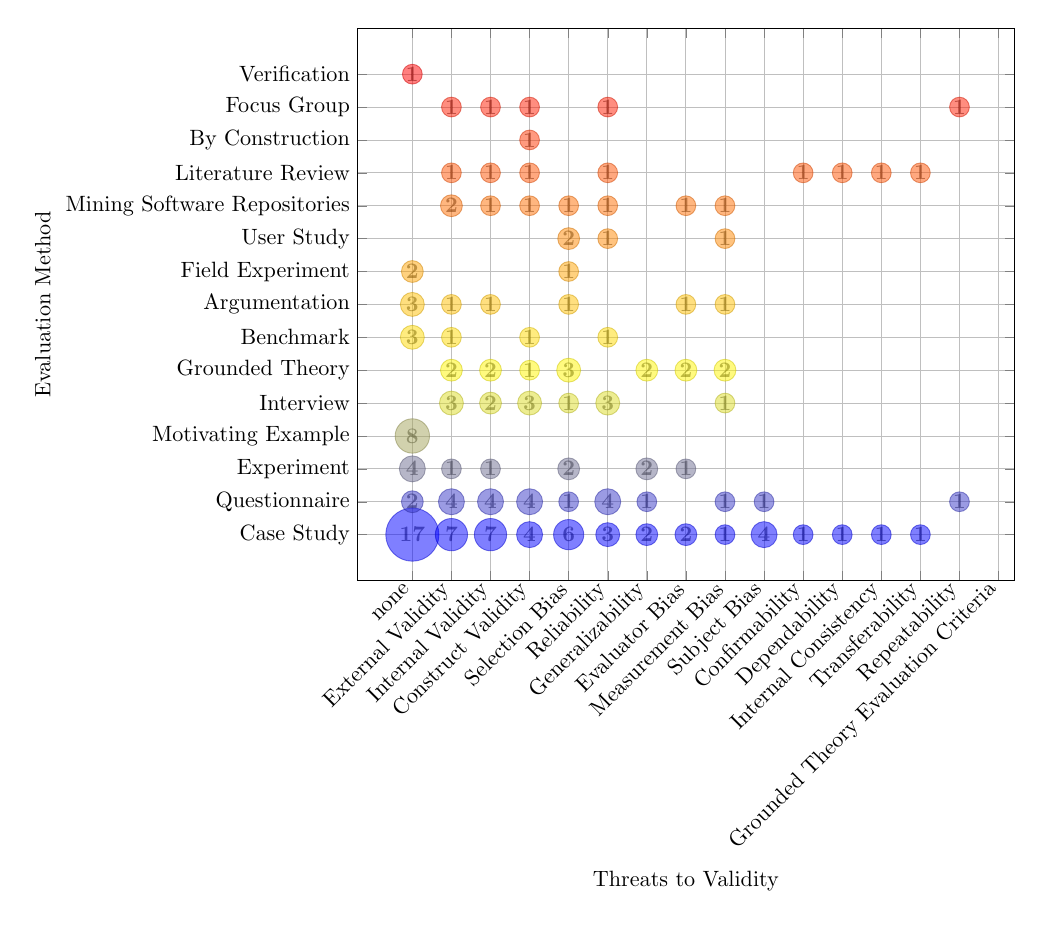
\begin{tikzpicture}[scale=.8]
\begin{axis}[scatter,
    width=.99\linewidth,
    cycle multi list=Spectral,
    every axis plot/.append style={draw, fill, fill opacity=0.5},
    scatter src=y,
    nodes near coords style={color=black,font=\small},
    %enlargelimits=0.15,
    x tick label style={rotate=45,anchor=east},
    xtick={0,1,2,3,4,5,6,7,8,9,10,11,12,13,14,15}, xticklabels={none,External Validity,Internal Validity,Construct Validity,Selection Bias,Reliability,Generalizability,Evaluator Bias,Measurement Bias,Subject Bias,Confirmability,Dependability,Internal Consistency,Transferability,Repeatability,Grounded Theory Evaluation Criteria},
    xlabel={Threats to Validity},
    ytick={0,1,2,3,4,5,6,7,8,9,10,11,12,13,14}, yticklabels={Case Study,Questionnaire,Experiment,Motivating Example,Interview,Grounded Theory,Benchmark,Argumentation,Field Experiment,User Study,Mining Software Repositories,Literature Review,By Construction,Focus Group,Verification},
    ylabel={Evaluation Method},
    grid=both
]

\addplot[mark size=12.000,opacity=0.5,text=black] coordinates { (0,0) } node[text=black,font=\bfseries] {17};
\addplot[mark size=4.941,opacity=0.5,text=black] coordinates { (0,1) } node[text=black,font=\bfseries] {2};
\addplot[mark size=5.882,opacity=0.5,text=black] coordinates { (0,2) } node[text=black,font=\bfseries] {4};
\addplot[mark size=7.765,opacity=0.5,text=black] coordinates { (0,3) } node[text=black,font=\bfseries] {8};
\addplot[mark size=5.412,opacity=0.5,text=black] coordinates { (0,6) } node[text=black,font=\bfseries] {3};
\addplot[mark size=5.412,opacity=0.5,text=black] coordinates { (0,7) } node[text=black,font=\bfseries] {3};
\addplot[mark size=4.941,opacity=0.5,text=black] coordinates { (0,8) } node[text=black,font=\bfseries] {2};
\addplot[mark size=4.471,opacity=0.5,text=black] coordinates { (0,14) } node[text=black,font=\bfseries] {1};
\addplot[mark size=7.294,opacity=0.5,text=black] coordinates { (1,0) } node[text=black,font=\bfseries] {7};
\addplot[mark size=5.882,opacity=0.5,text=black] coordinates { (1,1) } node[text=black,font=\bfseries] {4};
\addplot[mark size=4.471,opacity=0.5,text=black] coordinates { (1,2) } node[text=black,font=\bfseries] {1};
\addplot[mark size=5.412,opacity=0.5,text=black] coordinates { (1,4) } node[text=black,font=\bfseries] {3};
\addplot[mark size=4.941,opacity=0.5,text=black] coordinates { (1,5) } node[text=black,font=\bfseries] {2};
\addplot[mark size=4.471,opacity=0.5,text=black] coordinates { (1,6) } node[text=black,font=\bfseries] {1};
\addplot[mark size=4.471,opacity=0.5,text=black] coordinates { (1,7) } node[text=black,font=\bfseries] {1};
\addplot[mark size=4.941,opacity=0.5,text=black] coordinates { (1,10) } node[text=black,font=\bfseries] {2};
\addplot[mark size=4.471,opacity=0.5,text=black] coordinates { (1,11) } node[text=black,font=\bfseries] {1};
\addplot[mark size=4.471,opacity=0.5,text=black] coordinates { (1,13) } node[text=black,font=\bfseries] {1};
\addplot[mark size=7.294,opacity=0.5,text=black] coordinates { (2,0) } node[text=black,font=\bfseries] {7};
\addplot[mark size=5.882,opacity=0.5,text=black] coordinates { (2,1) } node[text=black,font=\bfseries] {4};
\addplot[mark size=4.471,opacity=0.5,text=black] coordinates { (2,2) } node[text=black,font=\bfseries] {1};
\addplot[mark size=4.941,opacity=0.5,text=black] coordinates { (2,4) } node[text=black,font=\bfseries] {2};
\addplot[mark size=4.941,opacity=0.5,text=black] coordinates { (2,5) } node[text=black,font=\bfseries] {2};
\addplot[mark size=4.471,opacity=0.5,text=black] coordinates { (2,7) } node[text=black,font=\bfseries] {1};
\addplot[mark size=4.471,opacity=0.5,text=black] coordinates { (2,10) } node[text=black,font=\bfseries] {1};
\addplot[mark size=4.471,opacity=0.5,text=black] coordinates { (2,11) } node[text=black,font=\bfseries] {1};
\addplot[mark size=4.471,opacity=0.5,text=black] coordinates { (2,13) } node[text=black,font=\bfseries] {1};
\addplot[mark size=5.882,opacity=0.5,text=black] coordinates { (3,0) } node[text=black,font=\bfseries] {4};
\addplot[mark size=5.882,opacity=0.5,text=black] coordinates { (3,1) } node[text=black,font=\bfseries] {4};
\addplot[mark size=5.412,opacity=0.5,text=black] coordinates { (3,4) } node[text=black,font=\bfseries] {3};
\addplot[mark size=4.471,opacity=0.5,text=black] coordinates { (3,5) } node[text=black,font=\bfseries] {1};
\addplot[mark size=4.471,opacity=0.5,text=black] coordinates { (3,6) } node[text=black,font=\bfseries] {1};
\addplot[mark size=4.471,opacity=0.5,text=black] coordinates { (3,10) } node[text=black,font=\bfseries] {1};
\addplot[mark size=4.471,opacity=0.5,text=black] coordinates { (3,11) } node[text=black,font=\bfseries] {1};
\addplot[mark size=4.471,opacity=0.5,text=black] coordinates { (3,12) } node[text=black,font=\bfseries] {1};
\addplot[mark size=4.471,opacity=0.5,text=black] coordinates { (3,13) } node[text=black,font=\bfseries] {1};
\addplot[mark size=6.824,opacity=0.5,text=black] coordinates { (4,0) } node[text=black,font=\bfseries] {6};
\addplot[mark size=4.471,opacity=0.5,text=black] coordinates { (4,1) } node[text=black,font=\bfseries] {1};
\addplot[mark size=4.941,opacity=0.5,text=black] coordinates { (4,2) } node[text=black,font=\bfseries] {2};
\addplot[mark size=4.471,opacity=0.5,text=black] coordinates { (4,4) } node[text=black,font=\bfseries] {1};
\addplot[mark size=5.412,opacity=0.5,text=black] coordinates { (4,5) } node[text=black,font=\bfseries] {3};
\addplot[mark size=4.471,opacity=0.5,text=black] coordinates { (4,7) } node[text=black,font=\bfseries] {1};
\addplot[mark size=4.471,opacity=0.5,text=black] coordinates { (4,8) } node[text=black,font=\bfseries] {1};
\addplot[mark size=4.941,opacity=0.5,text=black] coordinates { (4,9) } node[text=black,font=\bfseries] {2};
\addplot[mark size=4.471,opacity=0.5,text=black] coordinates { (4,10) } node[text=black,font=\bfseries] {1};
\addplot[mark size=5.412,opacity=0.5,text=black] coordinates { (5,0) } node[text=black,font=\bfseries] {3};
\addplot[mark size=5.882,opacity=0.5,text=black] coordinates { (5,1) } node[text=black,font=\bfseries] {4};
\addplot[mark size=5.412,opacity=0.5,text=black] coordinates { (5,4) } node[text=black,font=\bfseries] {3};
\addplot[mark size=4.471,opacity=0.5,text=black] coordinates { (5,6) } node[text=black,font=\bfseries] {1};
\addplot[mark size=4.471,opacity=0.5,text=black] coordinates { (5,9) } node[text=black,font=\bfseries] {1};
\addplot[mark size=4.471,opacity=0.5,text=black] coordinates { (5,10) } node[text=black,font=\bfseries] {1};
\addplot[mark size=4.471,opacity=0.5,text=black] coordinates { (5,11) } node[text=black,font=\bfseries] {1};
\addplot[mark size=4.471,opacity=0.5,text=black] coordinates { (5,13) } node[text=black,font=\bfseries] {1};
\addplot[mark size=4.941,opacity=0.5,text=black] coordinates { (6,0) } node[text=black,font=\bfseries] {2};
\addplot[mark size=4.471,opacity=0.5,text=black] coordinates { (6,1) } node[text=black,font=\bfseries] {1};
\addplot[mark size=4.941,opacity=0.5,text=black] coordinates { (6,2) } node[text=black,font=\bfseries] {2};
\addplot[mark size=4.941,opacity=0.5,text=black] coordinates { (6,5) } node[text=black,font=\bfseries] {2};
\addplot[mark size=4.941,opacity=0.5,text=black] coordinates { (7,0) } node[text=black,font=\bfseries] {2};
\addplot[mark size=4.471,opacity=0.5,text=black] coordinates { (7,2) } node[text=black,font=\bfseries] {1};
\addplot[mark size=4.941,opacity=0.5,text=black] coordinates { (7,5) } node[text=black,font=\bfseries] {2};
\addplot[mark size=4.471,opacity=0.5,text=black] coordinates { (7,7) } node[text=black,font=\bfseries] {1};
\addplot[mark size=4.471,opacity=0.5,text=black] coordinates { (7,10) } node[text=black,font=\bfseries] {1};
\addplot[mark size=4.471,opacity=0.5,text=black] coordinates { (8,0) } node[text=black,font=\bfseries] {1};
\addplot[mark size=4.471,opacity=0.5,text=black] coordinates { (8,1) } node[text=black,font=\bfseries] {1};
\addplot[mark size=4.471,opacity=0.5,text=black] coordinates { (8,4) } node[text=black,font=\bfseries] {1};
\addplot[mark size=4.941,opacity=0.5,text=black] coordinates { (8,5) } node[text=black,font=\bfseries] {2};
\addplot[mark size=4.471,opacity=0.5,text=black] coordinates { (8,7) } node[text=black,font=\bfseries] {1};
\addplot[mark size=4.471,opacity=0.5,text=black] coordinates { (8,9) } node[text=black,font=\bfseries] {1};
\addplot[mark size=4.471,opacity=0.5,text=black] coordinates { (8,10) } node[text=black,font=\bfseries] {1};
\addplot[mark size=5.882,opacity=0.5,text=black] coordinates { (9,0) } node[text=black,font=\bfseries] {4};
\addplot[mark size=4.471,opacity=0.5,text=black] coordinates { (9,1) } node[text=black,font=\bfseries] {1};
\addplot[mark size=4.471,opacity=0.5,text=black] coordinates { (10,0) } node[text=black,font=\bfseries] {1};
\addplot[mark size=4.471,opacity=0.5,text=black] coordinates { (10,11) } node[text=black,font=\bfseries] {1};
\addplot[mark size=4.471,opacity=0.5,text=black] coordinates { (11,0) } node[text=black,font=\bfseries] {1};
\addplot[mark size=4.471,opacity=0.5,text=black] coordinates { (11,11) } node[text=black,font=\bfseries] {1};
\addplot[mark size=4.471,opacity=0.5,text=black] coordinates { (12,0) } node[text=black,font=\bfseries] {1};
\addplot[mark size=4.471,opacity=0.5,text=black] coordinates { (12,11) } node[text=black,font=\bfseries] {1};
\addplot[mark size=4.471,opacity=0.5,text=black] coordinates { (13,0) } node[text=black,font=\bfseries] {1};
\addplot[mark size=4.471,opacity=0.5,text=black] coordinates { (13,11) } node[text=black,font=\bfseries] {1};
\addplot[mark size=4.471,opacity=0.5,text=black] coordinates { (14,1) } node[text=black,font=\bfseries] {1};
\addplot[mark size=4.471,opacity=0.5,text=black] coordinates { (14,13) } node[text=black,font=\bfseries] {1};


\end{axis}
\end{tikzpicture}
\end{center}
%\caption{Portfolio f\"ur Threats to Validity und Evaluation Method (Gr\"o\ss{}e entspricht der Anzahl)}\label{fig:port_threatstovalidity_evaluationmethod}
%\end{figure}


%\subsection{Portfolio f\"ur Replication Package und Evaluation Method (Gr\"o\ss{}e entspricht der Anzahl)}
%\begin{figure}
\begin{center}
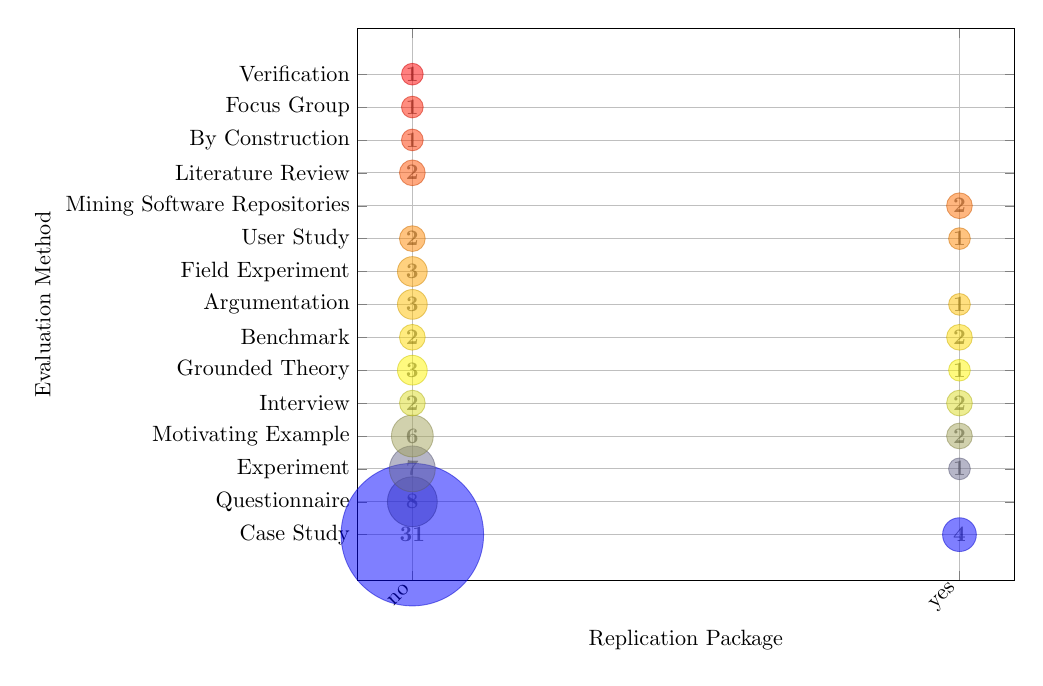
\begin{tikzpicture}[scale=.8]
\begin{axis}[scatter,
    width=.99\linewidth,
    cycle multi list=Spectral,
    every axis plot/.append style={draw, fill, fill opacity=0.5},
    scatter src=y,
    nodes near coords style={color=black,font=\small},
    %enlargelimits=0.15,
    x tick label style={rotate=45,anchor=east},
    xtick={0,1}, xticklabels={no,yes},
    xlabel={Replication Package},
    ytick={0,1,2,3,4,5,6,7,8,9,10,11,12,13,14}, yticklabels={Case Study,Questionnaire,Experiment,Motivating Example,Interview,Grounded Theory,Benchmark,Argumentation,Field Experiment,User Study,Mining Software Repositories,Literature Review,By Construction,Focus Group,Verification},
    ylabel={Evaluation Method},
    grid=both
]

\addplot[mark size=32.182,opacity=0.5,text=black] coordinates { (0,0) } node[text=black,font=\bfseries] {31};
\addplot[mark size=11.273,opacity=0.5,text=black] coordinates { (0,1) } node[text=black,font=\bfseries] {8};
\addplot[mark size=10.364,opacity=0.5,text=black] coordinates { (0,2) } node[text=black,font=\bfseries] {7};
\addplot[mark size=9.455,opacity=0.5,text=black] coordinates { (0,3) } node[text=black,font=\bfseries] {6};
\addplot[mark size=5.818,opacity=0.5,text=black] coordinates { (0,4) } node[text=black,font=\bfseries] {2};
\addplot[mark size=6.727,opacity=0.5,text=black] coordinates { (0,5) } node[text=black,font=\bfseries] {3};
\addplot[mark size=5.818,opacity=0.5,text=black] coordinates { (0,6) } node[text=black,font=\bfseries] {2};
\addplot[mark size=6.727,opacity=0.5,text=black] coordinates { (0,7) } node[text=black,font=\bfseries] {3};
\addplot[mark size=6.727,opacity=0.5,text=black] coordinates { (0,8) } node[text=black,font=\bfseries] {3};
\addplot[mark size=5.818,opacity=0.5,text=black] coordinates { (0,9) } node[text=black,font=\bfseries] {2};
\addplot[mark size=5.818,opacity=0.5,text=black] coordinates { (0,11) } node[text=black,font=\bfseries] {2};
\addplot[mark size=4.909,opacity=0.5,text=black] coordinates { (0,12) } node[text=black,font=\bfseries] {1};
\addplot[mark size=4.909,opacity=0.5,text=black] coordinates { (0,13) } node[text=black,font=\bfseries] {1};
\addplot[mark size=4.909,opacity=0.5,text=black] coordinates { (0,14) } node[text=black,font=\bfseries] {1};
\addplot[mark size=7.636,opacity=0.5,text=black] coordinates { (1,0) } node[text=black,font=\bfseries] {4};
\addplot[mark size=4.909,opacity=0.5,text=black] coordinates { (1,2) } node[text=black,font=\bfseries] {1};
\addplot[mark size=5.818,opacity=0.5,text=black] coordinates { (1,3) } node[text=black,font=\bfseries] {2};
\addplot[mark size=5.818,opacity=0.5,text=black] coordinates { (1,4) } node[text=black,font=\bfseries] {2};
\addplot[mark size=4.909,opacity=0.5,text=black] coordinates { (1,5) } node[text=black,font=\bfseries] {1};
\addplot[mark size=5.818,opacity=0.5,text=black] coordinates { (1,6) } node[text=black,font=\bfseries] {2};
\addplot[mark size=4.909,opacity=0.5,text=black] coordinates { (1,7) } node[text=black,font=\bfseries] {1};
\addplot[mark size=4.909,opacity=0.5,text=black] coordinates { (1,9) } node[text=black,font=\bfseries] {1};
\addplot[mark size=5.818,opacity=0.5,text=black] coordinates { (1,10) } node[text=black,font=\bfseries] {2};


\end{axis}
\end{tikzpicture}
\end{center}
%\caption{Portfolio f\"ur Replication Package und Evaluation Method (Gr\"o\ss{}e entspricht der Anzahl)}\label{fig:port_replicationpackage_evaluationmethod}
%\end{figure}



\section{Guidelines for Evaluation Methods and Threats to Validity}

%\subsection{Histogramm f\"ur Evaluation Guideline (76)}
%\begin{figure}
\begin{center}
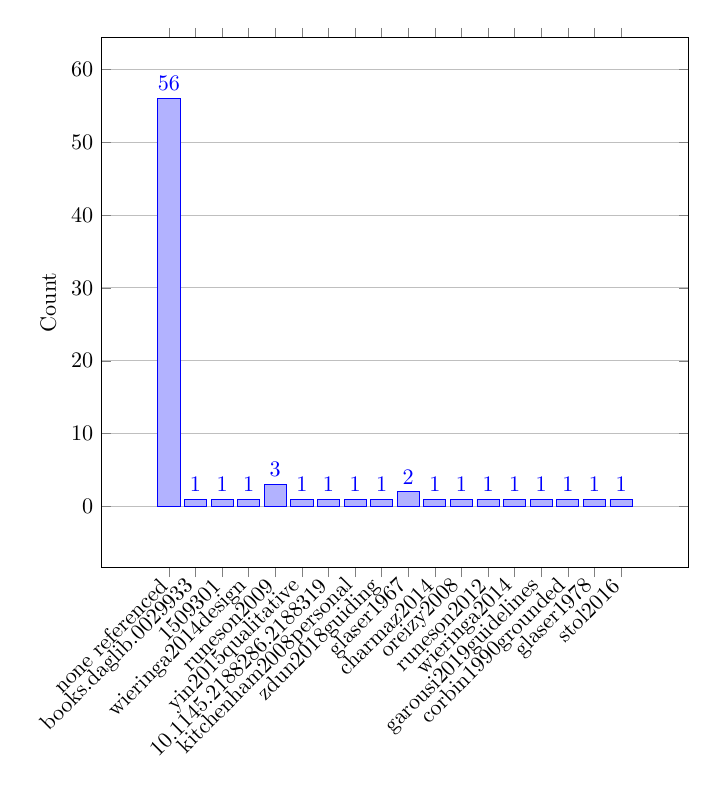
\begin{tikzpicture}[scale=.8]
\begin{axis}[ ybar, ymajorgrids, enlargelimits=0.15, legend style={at={(0.5,-0.15)}, anchor=north,legend columns=-1},
    width=.90\linewidth,height=10cm,
    nodes near coords, %nodes near coords align=below,
    ylabel={Count}, ymin=0,
    x tick label style={rotate=45,anchor=east},
    xtick={1,2,3,4,5,6,7,8,9,10,11,12,13,14,15,16,17,18},
    xticklabels={ none referenced, books.daglib.0029933, 1509301, wieringa2014design, runeson2009, yin2015qualitative, 10.1145.2188286.2188319, kitchenham2008personal, zdun2018guiding, glaser1967, charmaz2014, oreizy2008, runeson2012, wieringa2014, garousi2019guidelines, corbin1990grounded, glaser1978, stol2016
}
    %xlabel={Evaluation Guideline}    
    ]
  \addplot coordinates { (1,56)  (2,1)  (3,1)  (4,1)  (5,3)  (6,1)  (7,1)  (8,1)  (9,1)  (10,2)  (11,1)  (12,1)  (13,1)  (14,1)  (15,1)  (16,1)  (17,1)  (18,1)   };
\end{axis}
\end{tikzpicture}
\end{center}
%\caption{Histogramm f\"ur Evaluation Guideline (76)}
%\label{fig:histo_evaluationguideline}
%\end{figure}


%\subsection{Histogramm f\"ur Threats to Validity Guideline (68)}
%\begin{figure}
\begin{center}
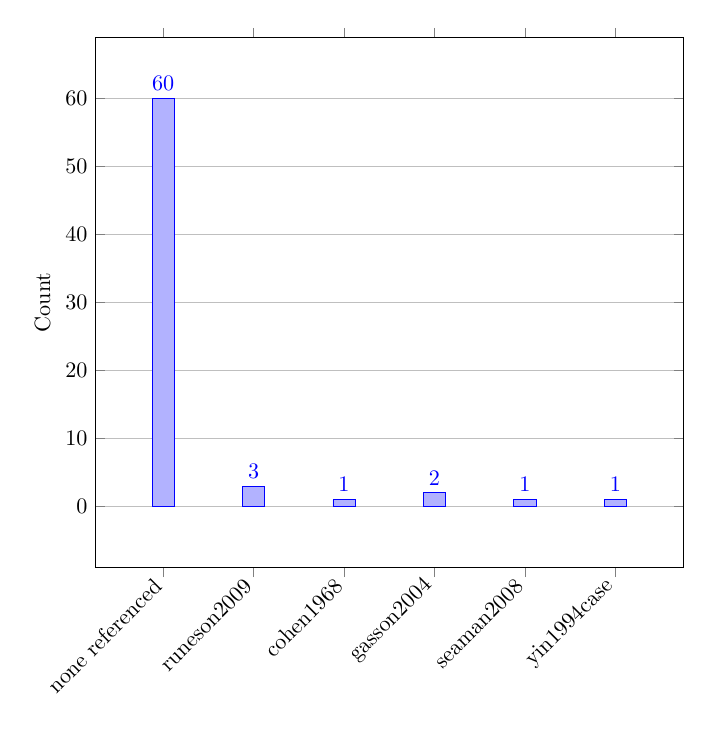
\begin{tikzpicture}[scale=.8]
\begin{axis}[ ybar, ymajorgrids, enlargelimits=0.15, legend style={at={(0.5,-0.15)}, anchor=north,legend columns=-1},
    width=.90\linewidth,height=10cm,
    nodes near coords, %nodes near coords align=below,
    ylabel={Count}, ymin=0,
    x tick label style={rotate=45,anchor=east},
    xtick={1,2,3,4,5,6},
    xticklabels={ none referenced, runeson2009, cohen1968, gasson2004, seaman2008, yin1994case
}
    %xlabel={Threats to Validity Guideline}    
    ]
  \addplot coordinates { (1,60)  (2,3)  (3,1)  (4,2)  (5,1)  (6,1)   };
\end{axis}
\end{tikzpicture}
\end{center}
%\caption{Histogramm f\"ur Threats to Validity Guideline (68)}
%\label{fig:histo_threatstovalidityguideline}
%\end{figure}


%\subsection{Pie chart for Evaluation Guideline (76)}
%\begin{figure}
\begin{center}
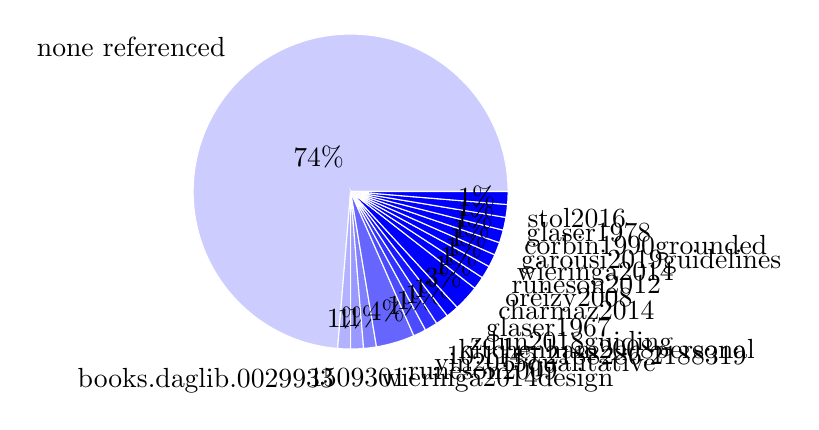
\begin{tikzpicture}[scale=2]
\pgfmathsetcounter{pieh}{0}
\foreach \p/\q/\t/\c in {74/56/none referenced/blue!20, 1/1/books.daglib.0029933/blue!30, 1/1/1509301/blue!40, 1/1/wieringa2014design/blue!50, 4/3/runeson2009/blue!60, 1/1/yin2015qualitative/blue!70, 1/1/10.1145.2188286.2188319/blue!80, 1/1/kitchenham2008personal/blue!90, 1/1/zdun2018guiding/blue!100, 3/2/glaser1967/blue!110, 1/1/charmaz2014/blue!120, 1/1/oreizy2008/blue!130, 1/1/runeson2012/blue!140, 1/1/wieringa2014/blue!150, 1/1/garousi2019guidelines/blue!160, 1/1/corbin1990grounded/blue!170, 1/1/glaser1978/blue!180, 1/1/stol2016/blue!190}
  {
    \setcounter{pieg}{\value{pieh}}
    \addtocounter{pieh}{\q}
    \slice{\thepieg/76*360}
          {\thepieh/76*360}
          {\p\%}{\t}{\c}
  }
\end{tikzpicture}

\textbf{Pie chart for Evaluation Guideline (76)}
\end{center}
%\caption{Pie chart for Evaluation Guideline (76)}
%\label{fig:pie_evaluationguideline}
%\end{figure}


%\subsection{Pie chart for Threats to Validity Guideline (68)}
%\begin{figure}
\begin{center}
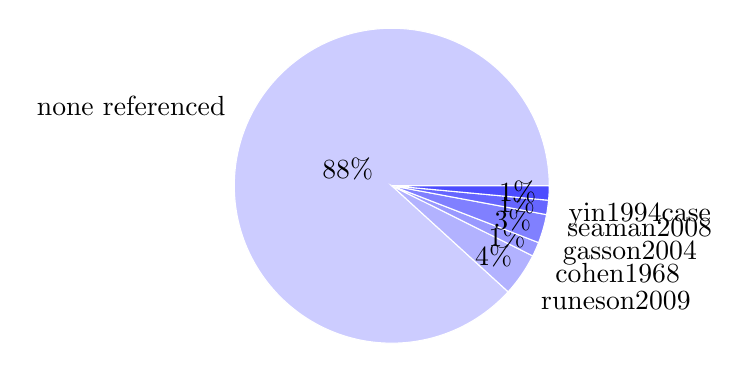
\begin{tikzpicture}[scale=2]
\pgfmathsetcounter{pieh}{0}
\foreach \p/\q/\t/\c in {88/60/none referenced/blue!20, 4/3/runeson2009/blue!30, 1/1/cohen1968/blue!40, 3/2/gasson2004/blue!50, 1/1/seaman2008/blue!60, 1/1/yin1994case/blue!70}
  {
    \setcounter{pieg}{\value{pieh}}
    \addtocounter{pieh}{\q}
    \slice{\thepieg/68*360}
          {\thepieh/68*360}
          {\p\%}{\t}{\c}
  }
\end{tikzpicture}

\textbf{Pie chart for Threats to Validity Guideline (68)}
\end{center}
%\caption{Pie chart for Threats to Validity Guideline (68)}
%\label{fig:pie_threatstovalidityguideline}
%\end{figure}


%\subsection{Histogram von Year je Evaluation Guideline}
%\begin{figure}
\begin{center}
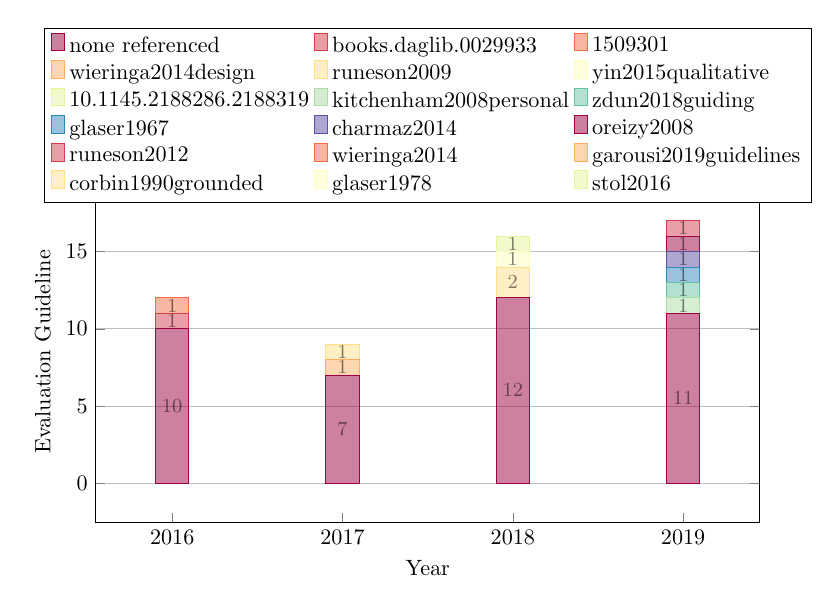
\begin{tikzpicture}[scale=0.8]
\
\begin{axis}[ width=\linewidth,height=7cm, ybar stacked,
    cycle multi list=Spectral,
    every axis plot/.append style={draw, fill, fill opacity=0.5},
    enlargelimits=0.15, 
    bar width=1.5em,
    nodes near coords, %nodes near coords align=below,
    nodes near coords style={color=black,font=\small},
    legend style={at={(0.5,1.45)}, anchor=north,legend columns=3},
    legend cell align={left},
    ylabel={Evaluation Guideline},ymajorgrids,ymin=0,
    %x tick label style={rotate=45,anchor=east},
    ymin=0,
    xtick={1,2,3,4}, xticklabels={2016,2017,2018,2019},
    xlabel={Year}    
   ]
\addplot coordinates { (1,10)  (2,7)  (3,12)  (4,11)  };
\addplot coordinates { (1,1)  (2,0)  (3,0)  (4,0)  };
\addplot coordinates { (1,1)  (2,0)  (3,0)  (4,0)  };
\addplot coordinates { (1,0)  (2,1)  (3,0)  (4,0)  };
\addplot coordinates { (1,0)  (2,1)  (3,2)  (4,0)  };
\addplot coordinates { (1,0)  (2,0)  (3,1)  (4,0)  };
\addplot coordinates { (1,0)  (2,0)  (3,1)  (4,0)  };
\addplot coordinates { (1,0)  (2,0)  (3,0)  (4,1)  };
\addplot coordinates { (1,0)  (2,0)  (3,0)  (4,1)  };
\addplot coordinates { (1,0)  (2,0)  (3,0)  (4,1)  };
\addplot coordinates { (1,0)  (2,0)  (3,0)  (4,1)  };
\addplot coordinates { (1,0)  (2,0)  (3,0)  (4,1)  };
\addplot coordinates { (1,0)  (2,0)  (3,0)  (4,1)  };
\addplot coordinates { (1,0)  (2,0)  (3,0)  (4,0)  };
\addplot coordinates { (1,0)  (2,0)  (3,0)  (4,0)  };
\addplot coordinates { (1,0)  (2,0)  (3,0)  (4,0)  };
\addplot coordinates { (1,0)  (2,0)  (3,0)  (4,0)  };
\addplot coordinates { (1,0)  (2,0)  (3,0)  (4,0)  };

\legend{none referenced,books.daglib.0029933,1509301,wieringa2014design,runeson2009,yin2015qualitative,10.1145.2188286.2188319,kitchenham2008personal,zdun2018guiding,glaser1967,charmaz2014,oreizy2008,runeson2012,wieringa2014,garousi2019guidelines,corbin1990grounded,glaser1978,stol2016}
\end{axis}
\end{tikzpicture}
\end{center}
%\caption{Histogram von Year je Evaluation Guideline}
%\label{fig:chisto_year_evaluationguideline}
%\end{figure}


%\subsection{Histogram von Year je Threats to Validity Guideline}
%\begin{figure}
\begin{center}
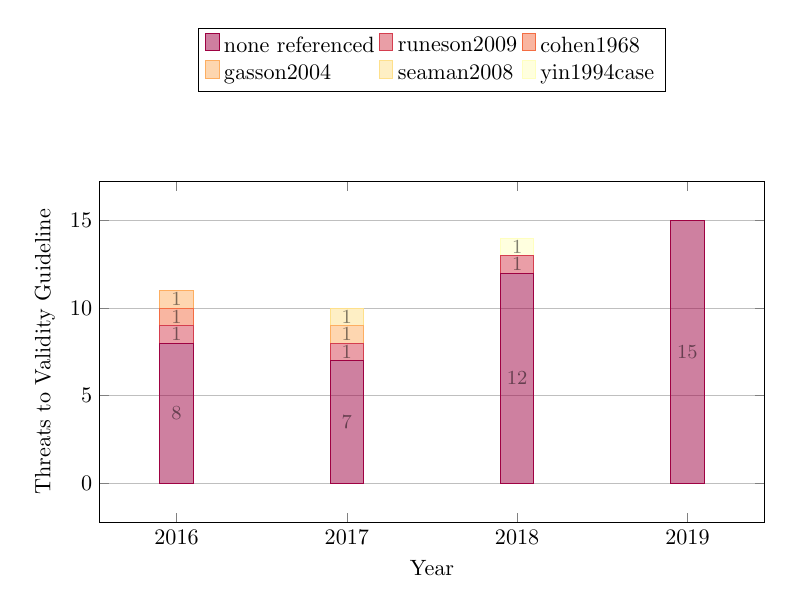
\begin{tikzpicture}[scale=0.8]
\
\begin{axis}[ width=\linewidth,height=7cm, ybar stacked,
    cycle multi list=Spectral,
    every axis plot/.append style={draw, fill, fill opacity=0.5},
    enlargelimits=0.15, 
    bar width=1.5em,
    nodes near coords, %nodes near coords align=below,
    nodes near coords style={color=black,font=\small},
    legend style={at={(0.5,1.45)}, anchor=north,legend columns=3},
    legend cell align={left},
    ylabel={Threats to Validity Guideline},ymajorgrids,ymin=0,
    %x tick label style={rotate=45,anchor=east},
    ymin=0,
    xtick={1,2,3,4}, xticklabels={2016,2017,2018,2019},
    xlabel={Year}    
   ]
\addplot coordinates { (1,8)  (2,7)  (3,12)  (4,15)  };
\addplot coordinates { (1,1)  (2,1)  (3,1)  (4,0)  };
\addplot coordinates { (1,1)  (2,0)  (3,0)  (4,0)  };
\addplot coordinates { (1,1)  (2,1)  (3,0)  (4,0)  };
\addplot coordinates { (1,0)  (2,1)  (3,0)  (4,0)  };
\addplot coordinates { (1,0)  (2,0)  (3,1)  (4,0)  };

\legend{none referenced,runeson2009,cohen1968,gasson2004,seaman2008,yin1994case}
\end{axis}
\end{tikzpicture}
\end{center}
%\caption{Histogram von Year je Threats to Validity Guideline}
%\label{fig:chisto_year_threatstovalidityguideline}
%\end{figure}


%\subsection{Portfolio f\"ur Evaluation Guideline und Threats to Validity Guideline (Gr\"o\ss{}e entspricht der Anzahl)}
%\begin{figure}
\begin{center}
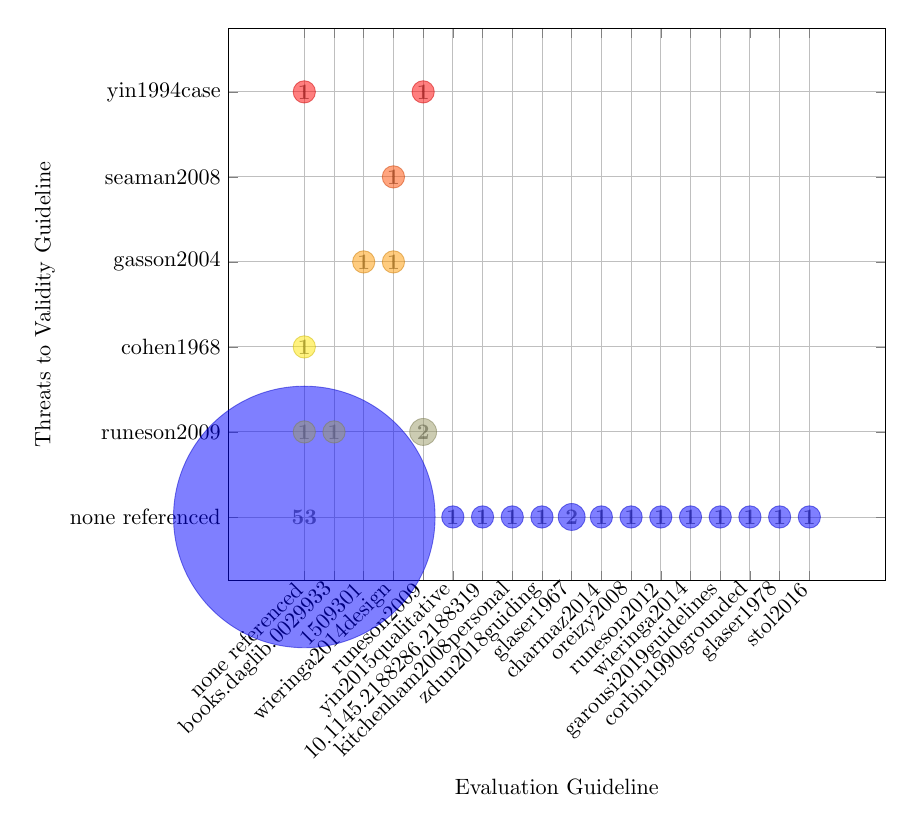
\begin{tikzpicture}[scale=.8]
\begin{axis}[scatter,
    width=.99\linewidth,
    cycle multi list=Spectral,
    every axis plot/.append style={draw, fill, fill opacity=0.5},
    scatter src=y,
    nodes near coords style={color=black,font=\small},
    enlargelimits=0.15,
    x tick label style={rotate=45,anchor=east},
    xtick={0,1,2,3,4,5,6,7,8,9,10,11,12,13,14,15,16,17}, xticklabels={none referenced,books.daglib.0029933,1509301,wieringa2014design,runeson2009,yin2015qualitative,10.1145.2188286.2188319,kitchenham2008personal,zdun2018guiding,glaser1967,charmaz2014,oreizy2008,runeson2012,wieringa2014,garousi2019guidelines,corbin1990grounded,glaser1978,stol2016},
    xlabel={Evaluation Guideline},
    ytick={0,1,2,3,4,5}, yticklabels={none referenced,runeson2009,cohen1968,gasson2004,seaman2008,yin1994case},
    ylabel={Threats to Validity Guideline},
    grid=both
]

\addplot[mark size=59.065,opacity=0.5,text=black] coordinates { (0,0) } node[text=black,font=\bfseries] {53};
\addplot[mark size=5.039,opacity=0.5,text=black] coordinates { (0,1) } node[text=black,font=\bfseries] {1};
\addplot[mark size=5.039,opacity=0.5,text=black] coordinates { (0,2) } node[text=black,font=\bfseries] {1};
\addplot[mark size=5.039,opacity=0.5,text=black] coordinates { (0,5) } node[text=black,font=\bfseries] {1};
\addplot[mark size=5.039,opacity=0.5,text=black] coordinates { (1,1) } node[text=black,font=\bfseries] {1};
\addplot[mark size=5.039,opacity=0.5,text=black] coordinates { (2,3) } node[text=black,font=\bfseries] {1};
\addplot[mark size=5.039,opacity=0.5,text=black] coordinates { (3,3) } node[text=black,font=\bfseries] {1};
\addplot[mark size=5.039,opacity=0.5,text=black] coordinates { (3,4) } node[text=black,font=\bfseries] {1};
\addplot[mark size=6.078,opacity=0.5,text=black] coordinates { (4,1) } node[text=black,font=\bfseries] {2};
\addplot[mark size=5.039,opacity=0.5,text=black] coordinates { (4,5) } node[text=black,font=\bfseries] {1};
\addplot[mark size=5.039,opacity=0.5,text=black] coordinates { (5,0) } node[text=black,font=\bfseries] {1};
\addplot[mark size=5.039,opacity=0.5,text=black] coordinates { (6,0) } node[text=black,font=\bfseries] {1};
\addplot[mark size=5.039,opacity=0.5,text=black] coordinates { (7,0) } node[text=black,font=\bfseries] {1};
\addplot[mark size=5.039,opacity=0.5,text=black] coordinates { (8,0) } node[text=black,font=\bfseries] {1};
\addplot[mark size=6.078,opacity=0.5,text=black] coordinates { (9,0) } node[text=black,font=\bfseries] {2};
\addplot[mark size=5.039,opacity=0.5,text=black] coordinates { (10,0) } node[text=black,font=\bfseries] {1};
\addplot[mark size=5.039,opacity=0.5,text=black] coordinates { (11,0) } node[text=black,font=\bfseries] {1};
\addplot[mark size=5.039,opacity=0.5,text=black] coordinates { (12,0) } node[text=black,font=\bfseries] {1};
\addplot[mark size=5.039,opacity=0.5,text=black] coordinates { (13,0) } node[text=black,font=\bfseries] {1};
\addplot[mark size=5.039,opacity=0.5,text=black] coordinates { (14,0) } node[text=black,font=\bfseries] {1};
\addplot[mark size=5.039,opacity=0.5,text=black] coordinates { (15,0) } node[text=black,font=\bfseries] {1};
\addplot[mark size=5.039,opacity=0.5,text=black] coordinates { (16,0) } node[text=black,font=\bfseries] {1};
\addplot[mark size=5.039,opacity=0.5,text=black] coordinates { (17,0) } node[text=black,font=\bfseries] {1};


\end{axis}
\end{tikzpicture}
\end{center}
%\caption{Portfolio f\"ur Evaluation Guideline und Threats to Validity Guideline (Gr\"o\ss{}e entspricht der Anzahl)}\label{fig:port_evaluationguideline_threatstovalidityguideline}
%\end{figure}



\section{Table}

\begin{table}[p]
\tiny
\pgfplotstabletypeset[
  col sep=semicolon,
  string type,
  columns={Year, Paper ID, Research Objects, Evaluation Methods, Properties},
  columns/Year/.style={column name=Year, column type={l}},
  columns/Paper ID/.style={column name=Paper, column type={p{1.5em}}, postproc cell content/.style={@cell content={\cite{##1}}} },
  columns/Research Objects/.style={column name=Research Objects,column type={p{4.2cm}}},
  columns/Evaluation Methods/.style={column name=Evaluation Methods,column type={p{3.2cm}}},
  columns/Properties/.style={column name=Properties,column type={p{3.2cm}}},
  every head row/.style={before row=\toprule, after row=\midrule},
  every last row/.style={after row=\bottomrule},
]{data/Overview.csv}

\caption{Overview}
\end{table}

\bibliographystyle{unsrt}
\bibliography{ECSA-Proceedings}

\end{document}

